\documentclass[10pt,a4paper,spanish]{report}

\usepackage[spanish]{babel}
\usepackage[utf8]{inputenc}
\usepackage{amsmath, amsthm}
\usepackage{amsfonts, amssymb, latexsym}
\usepackage{enumerate}
% \usepackage[official]{eurosym}
\usepackage{graphicx}
\usepackage[usenames, dvipsnames]{color}
\usepackage{colortbl}
\usepackage{multirow}
\usepackage{fancyhdr}
\usepackage[all]{xy}
\usepackage{minted}
\usepackage{tikz}
\usepackage{pgfplots}
\usepackage{cancel}
\usepackage{subfigure}
\usepackage{wallpaper}
\usepackage{titlesec}
\titleformat{\chapter}[display]
  {\normalfont\huge\bfseries}{\chaptertitlename\ \thechapter}{20pt}{\Huge}
\titlespacing*{\chapter}{0pt}{-50pt}{40pt}
\pgfplotsset{compat=1.5}

\headsep 3mm
\marginparwidth 2.5mm
\oddsidemargin 3mm
\textwidth 150mm
\footskip 5mm

\usepackage[bookmarks=true,
            bookmarksnumbered=false, % true means bookmarks in
                                     % left window are numbered
            bookmarksopen=false,     % true means only level 1
                                     % are displayed.
            colorlinks=true,
            linkcolor=webblue]{hyperref}
\definecolor{webgreen}{rgb}{0, 0.5, 0} % less intense green
\definecolor{webblue}{rgb}{0, 0, 0.5}  % less intense blue
\definecolor{webred}{rgb}{0.5, 0, 0}   % less intense red

\newcommand{\HRule}{\rule{\linewidth}{0.5mm}} % regla horizontal para  el titulo

\pagestyle{fancy}
%con esto nos aseguramos de que las cabeceras de capítulo y de sección vayan en minúsculas

\renewcommand{\chaptermark}[1]{%
      \markboth{#1}{}}
\renewcommand{\sectionmark}[1]{%
      \markright{\thesection\ #1}}
\fancyhf{} %borra cabecera y pie actuales
\fancyhead[LE,RO]{{\bfseries\leftmark}}
\fancyhead[LO]{\bfseries Marta Gómez}
\fancyfoot[C]{\thepage{}}
\renewcommand{\headrulewidth}{0.5pt}
\renewcommand{\footrulewidth}{0pt}
\addtolength{\headheight}{0.5pt} %espacio para la raya
\fancypagestyle{plain}{%
      \fancyhead{} %elimina cabeceras en páginas "plain"
      \renewcommand{\headrulewidth}{0pt} %así como la raya
}

\newmintedfile[myc]{c}{
    linenos,
    numbersep=5pt,
    gobble=0,
    frame=lines,
    framesep=2mm,
    tabsize=3,
}

\newmintedfile[mylex]{bash}{
    linenos,
    numbersep=5pt,
    gobble=0,
    frame=lines,
    framesep=2mm,
    tabsize=3,
}

\newmintedfile[mylatex]{latex}{
    linenos,
    numbersep=5pt,
    gobble=0,
    frame=lines,
    framesep=2mm,
    tabsize=3,
}

\newmintedfile[myhtml]{html}{
    linenos,
    numbersep=5pt,
    gobble=0,
    frame=lines,
    framesep=2mm,
    tabsize=3,
}

\usepackage[sfdefault,light]{roboto}  %% Option 'sfdefault' only if the base font of the document is to be sans serif
\usepackage[T1]{fontenc}

\setlength{\parindent}{0pt}
\setlength{\parskip}{1ex plus 0.5ex minus 0.2ex}

%Definimos autor y título
\title{\Huge Prácticas de \\ Modelos de computación}
\author{Marta Gómez Macías}

\definecolor{p1}{rgb}{0.8, 0.0, 0.0}
\definecolor{p2}{rgb}{0.01, 0.28, 1.0}
\definecolor{p3}{rgb}{0.0, 0.42, 0.24}
\definecolor{p4}{rgb}{1.0, 0.13, 0.32}
\definecolor{p5}{rgb}{1.0, 0.22, 0.0}
\definecolor{p6}{rgb}{0.45, 0.31, 0.59}
\definecolor{p7}{rgb}{1.0, 0.77, 0.05}
\definecolor{p8}{rgb}{0.5, 0.0, 0.5}
\definecolor{p9}{rgb}{0.3, 0.73, 0.09}

\begin{document}
%Cambiar Cuadros por Tablas y lista de...
\renewcommand{\listtablename}{Índice de tablas}
\renewcommand{\tablename}{Tabla}
\renewcommand{\chaptername}{Práctica} 
\thispagestyle{empty}
\ThisCenterWallPaper{1.12}{portada.jpg} % Add the background image, the first argument is the scaling - adjust this as necessary so the image fits the entire page

\begin{tikzpicture}[remember picture,overlay]
\node [rectangle, rounded corners, fill=white, opacity=0.75, anchor=south west, minimum width=15cm, minimum height=6cm] (box) at (-2.5,-25) (box){}; % White rectangle - "minimum width/height" adjust the width and height of the box; "(-0.5,-10)" adjusts the position on the page
\node[anchor=west, xshift=-6.5cm, yshift=-0.7cm, text width=5cm] at (box.north){Universidad de Granada}; % "Text width" adjusts the wrapping width, "xshift/yshift" adjust the position relative to the white rectangle
\node[anchor=west, xshift=-6.5cm, yshift=-2.5cm, text width=13cm, font=\Huge] at (box.north){Prácticas de Modelos de Computación}; % "Text width" adjusts the wrapping width, "xshift/yshift" adjust the position relative to the white rectangle
\node[anchor=west, xshift=-6.5cm, yshift=-4.5cm, text width=5cm, font=\Large] at (box.north){Marta Gómez Macías}; % "Text width" adjusts the wrapping width, "xshift/yshift" adjust the position relative to the white rectangle
\end{tikzpicture}

\newpage % Make sure the following content is on a new page

\tableofcontents

% \listoffigures

% \listoftables

\newpage

\thispagestyle{empty}
\ThisULCornerWallPaper{1}{p1.jpg}

\begin{tikzpicture}[remember picture,overlay]
\node [rectangle, rounded corners, fill=white, opacity=0.75, anchor=south west, minimum width=7cm, minimum height=5cm] (box) at (-0.5,-1) (box){}; % White rectangle - "minimum width/height" adjust the width and height of the box; "(-0.5,-10)" adjusts the position on the page
\node[anchor=west, xshift=-3cm, yshift=-3cm, text width=5cm] at (box.north){\chapter{\textcolor{p1}{Gramáticas y lenguajes}}};
\end{tikzpicture}\\[2.5cm]

\section{\textcolor{p1}Enunciado}
Sea la gramática $G = (V,T,P,S)$, donde $V = \{S,A,B\}$, $T = \{a,b\}$, el símbolo de partida es $S$ y las reglas, $P$, son:
\begin{displaymath}
S \rightarrow aB, \qquad\ S \rightarrow bA, \qquad\ A \rightarrow a, \qquad A \rightarrow aS,
\end{displaymath}
\begin{displaymath}
A \rightarrow bAA, \qquad\ B \rightarrow b, \qquad\ B \rightarrow bS, \qquad\ B \rightarrow aBB
\end{displaymath}

Demostrar que esta gramática genera el lenguaje
\begin{displaymath}
  L(G) = \{u~ | ~u \in \{a,b\}^+ ~y~ N_a(u) = N_b(u) \}
\end{displaymath}
donde $N_a(u)$ y $N_b(u)$ son el número de apariciones de símbolos $a$ y $b$, en $u$, respectivamente y $\{a,b\}^+$ representa todas las cadenas existentes combinando $a$ y $b$ en cualquier orden excluyendo la cadena vacía ($\varepsilon$).

\section{\textcolor{p1}Solución}
En primer lugar, podemos elegir si queremos empezar por el símbolo $a$, con la regla $S \rightarrow aB$, o por el símbolo $b$, con la regla $S \rightarrow bA$.

A partir de ahí, siempre tendremos tantas variables $A$ o $B$ como símbolos $b$ o $a$ haya respectivamente. Esto quiere decir que siempre generaremos cadenas con el mismo número de símbolos $b$ como símbolos $a$.

Vamos a tratar de generar la cadena $bbbaa$ (3 símbolos $b$ y 2 símbolos $a$) para ver que es imposible llegar a ese resultado.

En primer lugar, empezaríamos por la regla que coloca un símbolo $b$ al inicio de la cadena:
\begin{displaymath}
S \rightarrow bA
\end{displaymath}

Después, tendríamos que sustituir la variable $A$ por una regla con la que podamos generar un símbolo $b$ más:
\begin{displaymath}
S \rightarrow bA \rightarrow bbAA
\end{displaymath}

Por último, nos queda conseguir el último símbolo $b$, para ello sustituimos la primera variable $A$ por la misma regla anterior:
\begin{displaymath}
S \rightarrow bA \rightarrow bbAA \rightarrow bbbAAA
\end{displaymath}

Ya tenemos todos los símbolos $b$ deseados, ahora sólo nos queda sustituir dos de las variables $A$ por símbolos $a$ para llegar al resultado deseado:
\begin{displaymath}
S \rightarrow bA \rightarrow bbAA \rightarrow bbbAAA \rightarrow bbbaaA
\end{displaymath}

Pero tenemos un problema: no hay ninguna regla para transformar una variable $A$ en la cadena vacía ($\varepsilon$), sólo tenemos las siguientes alternativas:
\begin{enumerate}[\color{p1}{$\heartsuit$}]
  \item Sustituir la variable $A$ por un símbolo $a$ y terminar nuestra cadena:
  \begin{displaymath}
  S \rightarrow bA \rightarrow bbAA \rightarrow bbbAAA \rightarrow bbbaaA \rightarrow bbbaaa
  \end{displaymath}
  
  \item Sustituir la variable $A$ por un símbolo $a$ y una variable $S$ para volver a empezar:
  \begin{displaymath}
  S \rightarrow bA \rightarrow bbAA \rightarrow bbbAAA \rightarrow bbbaaA \rightarrow bbbaaaS
  \end{displaymath}

  \item Sustituir la variable $A$ por un símbolo $b$ y dos variables $A$ más:
  \begin{displaymath}
  S \rightarrow bA \rightarrow bbAA \rightarrow bbbAAA \rightarrow bbbaaA \rightarrow bbbaabAA
  \end{displaymath}
\end{enumerate}

Por tanto, podemos concluir que es imposible obtener una cadena que cumpla la propiedad de $N_a(u) \neq N_b(u)$ con esta gramática.

\newpage

\thispagestyle{empty}
\ThisULCornerWallPaper{1}{p2.jpg}

\begin{tikzpicture}[remember picture,overlay]
\node [rectangle, rounded corners, fill=white, opacity=0.75, anchor=south west, minimum width=8cm, minimum height=4cm] (box) at (-0.5,-1) (box){}; % White rectangle - "minimum width/height" adjust the width and height of the box; "(-0.5,-10)" adjusts the position on the page
\node[anchor=west, xshift=-3.5cm, yshift=-2.5cm, text width=6cm] at (box.north){\chapter{\textcolor{p6}{Optimización de gramáticas}}};
\end{tikzpicture}\\[3cm]

\section{\textcolor{p6}Enunciado}
Determinar si la gramática $G = (\{S,A,B\}, \{a,b,c,d\}, P, S)$ donde $P$ es el conjunto de la reglas de producción:
\begin{displaymath}
S \rightarrow AB, \qquad\ A \rightarrow Ab, \qquad\ A \rightarrow a,
\end{displaymath}
\begin{displaymath}
B \rightarrow cB, \qquad B \rightarrow d
\end{displaymath}
genera un lenguage de tipo 3.

\section{\textcolor{p6}Solución}
Las dos primeras reglas de producción proporcionadas son libres de contexto (tipo 2), el resto, son regulares (tipo 3). Si modificamos estas reglas libres de contexto, nos quedará una gramática de tipo 3 capaz de generar el mismo tipo de lenguaje.

Ahora bien, antes de irnos a eso, vamos a ver qué lenguaje genera esta gramática.

Para empezar, sólo podemos sustituir el símbolo inicial $S$ por las variables $AB$:

\begin{displaymath}
S \rightarrow AB
\end{displaymath}

Después, podemos seguir por dos caminos:
\begin{enumerate}[\color{p6}{$\heartsuit$}]
  \item O bien sustituimos la variable $A$ por el símbolo terminal $a$:
  \begin{displaymath}
  S \rightarrow AB \rightarrow aB
  \end{displaymath}
  \item O bien, la sustituimos por otra variable $A$ y el símbolo terminal $b$
  \begin{displaymath}
  S \rightarrow AB \rightarrow AbB
  \end{displaymath}
\end{enumerate}

Si seguimos el segundo camino, llegamos a la misma situación anterior: o sustituir la variable $A$ por un símbolo terminal $a$ o sustituirla por otra variable $A$ acompañada de un símbolo terminal $b$. Así, podríamos entrar en un ciclo en el que tendríamos una variable $A$, un símbolo terminal $b$ repetido $i$ veces y, por último, una variable $B$. Para terminar este ciclo, sólo tendríamos que sustituir la variable $A$ por un símbolo terminal $a$, es decir, seguir el primer camino.

Por tanto, tendríamos la siguiente situación:

\begin{displaymath}
S \rightarrow AB \rightarrow Ab^iB \rightarrow ab^iB
\end{displaymath}

El siguiente paso sería sustituir la variable $B$, para ello, tenemos dos caminos:
\begin{enumerate}[\color{p6}{$\bigstar$}]
  \item Sustituir la variable $B$ por un símbolo terminal $d$.
  \item Sustituir la variable $B$ por un símbolo terminal $c$ acompañado de otra variable $B$.
\end{enumerate}

Así, llegamos a la misma situación anterior. Podemos entrar en el bucle del segundo camino y un símbolo terminal $c$ repetido $j$ veces y, para terminar, entrar al primer camino y finalizar con un símbolo terminal $d$.

En resumen, siguiendo estos pasos obtendríamos:

\begin{displaymath}
S \rightarrow AB \rightarrow Ab^iB \rightarrow ab^iB \rightarrow ab^ic^jB \rightarrow ab^ic^jd
\end{displaymath}

Por lo que podemos concluir diciendo que el lenguaje generado por esta gramática es:

\begin{equation*}
\{ab^ic^jd ~:~ i, j \in \mathbb{N}\}
\end{equation*}

Una vez sabido el lenguaje generado por la gramática, vamos a pensar una gramática regular que sea capaz de generar el mismo lenguaje.

La cadena empieza por el símbolo terminal $a$, por tanto el símbolo inicial $S$ debe poder sustituirse por el símbolo terminal $a$. Pero, también necesitamos crear el ciclo para repetir el símbolo terminal $b$ $i$ veces. Esto podemos hacerlo acompañando el símbolo terminal $a$ por una variable y haciendo otra regla para sustituir esa variable por el símbolo terminal $b$ acompañado de dicha variable para crear el bucle:

\begin{displaymath}
S \rightarrow aB, \qquad\ B \rightarrow bB
\end{displaymath}

Después, una vez hubiesemos conseguido repetir el símbolo terminal $b$ las $i$ veces deseadas, pasaríamos a hacer lo mismo con el símbolo terminal $c$. Para ello, deberíamos poder cambiar la variable $B$ por un símbolo terminal $c$ y hacer otro bucle, pero, si hacemos directamente con una regla $B \rightarrow cB$  podríamos generar cadenas de otro tipo. Por eso, hacemos un paso intermedio con una regla para transformar la variable $B$ en una variable $C$ y poder volver a empezar el mismo bucle, pero con el símbolo terminal $c$:

\begin{displaymath}
S \rightarrow aB, \qquad\ B \rightarrow bB, \qquad\ C \rightarrow B,
\end{displaymath}
\begin{displaymath}
C \rightarrow cC
\end{displaymath}

Por último, necesitaríamos una última regla para cambiar la variable $C$ por un símbolo terminal $d$ y así terminar nuestra cadena, para ello sólo necesitamos una regla que sustituya la variable $C$ por un símbolo terminal $d$.

Así, el conjunto de reglas para generar el lenguaje anterior sería:

\begin{displaymath}
S \rightarrow aB, \qquad\ B \rightarrow bB, \qquad\ C \rightarrow B,
\end{displaymath}
\begin{displaymath}
C \rightarrow cC, \qquad\ C \rightarrow d
\end{displaymath}

\newpage

\thispagestyle{empty}
\ThisULCornerWallPaper{1}{p3.jpg}

\begin{tikzpicture}[remember picture,overlay]
\node [rectangle, rounded corners, fill=white, opacity=0.75, anchor=south west, minimum width=12cm, minimum height=5cm] (box) at (-0.5,-1) (box){}; % White rectangle - "minimum width/height" adjust the width and height of the box; "(-0.5,-10)" adjusts the position on the page
\node[anchor=west, xshift=-5.5cm, yshift=-3.2cm, text width=10cm] at (box.north){\chapter{\textcolor{p3}{Autómatas finitos determinísticos y no determinísticos}}};
\end{tikzpicture}\\[3cm]

\section{\textcolor{p3}Enunciado}
Construir un autómata finito determinístico capaz de reconocer en una cadena de ceros y de unos la subcadena 0110. Y a continuación, no necesariamente seguido, la subcadena 1000. 

Para ello, se parte de los dos autómatas no determinísticos de la \hyperref[automatas]{Figura \ref*{automatas}}. El primero reconoce la subcadena 0110 en una cadena de ceros y unos. El segundo, la subcadena 1000.

\begin{figure}[!h]
\centering
% Graphic for TeX using PGF
% Title: /home/braulio/MEGA/Facultad/Tercero/Primer_Cuatrimestre/MC/Practicas/Diagrama_I.dia
% Creator: Dia v0.97.3
% CreationDate: Sat Oct 31 17:40:39 2015
% For: braulio
% \usepackage{tikz}
% The following commands are not supported in PSTricks at present
% We define them conditionally, so when they are implemented,
% this pgf file will use them.
\ifx\du\undefined
  \newlength{\du}
\fi
\setlength{\du}{15\unitlength}
\begin{tikzpicture}
\pgftransformxscale{1.000000}
\pgftransformyscale{-1.000000}
\definecolor{dialinecolor}{rgb}{0.000000, 0.000000, 0.000000}
\pgfsetstrokecolor{dialinecolor}
\definecolor{dialinecolor}{rgb}{1.000000, 1.000000, 1.000000}
\pgfsetfillcolor{dialinecolor}
\definecolor{dialinecolor}{rgb}{1.000000, 1.000000, 1.000000}
\pgfsetfillcolor{dialinecolor}
\pgfpathellipse{\pgfpoint{5.046634\du}{3.723322\du}}{\pgfpoint{1.303364\du}{0\du}}{\pgfpoint{0\du}{1.276682\du}}
\pgfusepath{fill}
\pgfsetlinewidth{0.100000\du}
\pgfsetdash{}{0pt}
\pgfsetdash{}{0pt}
\pgfsetmiterjoin
\definecolor{dialinecolor}{rgb}{0.000000, 0.000000, 0.000000}
\pgfsetstrokecolor{dialinecolor}
\pgfpathellipse{\pgfpoint{5.046634\du}{3.723322\du}}{\pgfpoint{1.303364\du}{0\du}}{\pgfpoint{0\du}{1.276682\du}}
\pgfusepath{stroke}
% setfont left to latex
\definecolor{dialinecolor}{rgb}{0.000000, 0.000000, 0.000000}
\pgfsetstrokecolor{dialinecolor}
\node at (5.046634\du,3.918322\du){q\_0};
\definecolor{dialinecolor}{rgb}{1.000000, 1.000000, 1.000000}
\pgfsetfillcolor{dialinecolor}
\pgfpathellipse{\pgfpoint{9.738364\du}{3.706682\du}}{\pgfpoint{1.303364\du}{0\du}}{\pgfpoint{0\du}{1.276682\du}}
\pgfusepath{fill}
\pgfsetlinewidth{0.100000\du}
\pgfsetdash{}{0pt}
\pgfsetdash{}{0pt}
\pgfsetmiterjoin
\definecolor{dialinecolor}{rgb}{0.000000, 0.000000, 0.000000}
\pgfsetstrokecolor{dialinecolor}
\pgfpathellipse{\pgfpoint{9.738364\du}{3.706682\du}}{\pgfpoint{1.303364\du}{0\du}}{\pgfpoint{0\du}{1.276682\du}}
\pgfusepath{stroke}
% setfont left to latex
\definecolor{dialinecolor}{rgb}{0.000000, 0.000000, 0.000000}
\pgfsetstrokecolor{dialinecolor}
\node at (9.738364\du,3.901682\du){q\_1};
\definecolor{dialinecolor}{rgb}{1.000000, 1.000000, 1.000000}
\pgfsetfillcolor{dialinecolor}
\pgfpathellipse{\pgfpoint{14.523364\du}{3.636682\du}}{\pgfpoint{1.303364\du}{0\du}}{\pgfpoint{0\du}{1.276682\du}}
\pgfusepath{fill}
\pgfsetlinewidth{0.100000\du}
\pgfsetdash{}{0pt}
\pgfsetdash{}{0pt}
\pgfsetmiterjoin
\definecolor{dialinecolor}{rgb}{0.000000, 0.000000, 0.000000}
\pgfsetstrokecolor{dialinecolor}
\pgfpathellipse{\pgfpoint{14.523364\du}{3.636682\du}}{\pgfpoint{1.303364\du}{0\du}}{\pgfpoint{0\du}{1.276682\du}}
\pgfusepath{stroke}
% setfont left to latex
\definecolor{dialinecolor}{rgb}{0.000000, 0.000000, 0.000000}
\pgfsetstrokecolor{dialinecolor}
\node at (14.523364\du,3.831682\du){q\_2};
\definecolor{dialinecolor}{rgb}{1.000000, 1.000000, 1.000000}
\pgfsetfillcolor{dialinecolor}
\pgfpathellipse{\pgfpoint{19.358364\du}{3.616682\du}}{\pgfpoint{1.303364\du}{0\du}}{\pgfpoint{0\du}{1.276682\du}}
\pgfusepath{fill}
\pgfsetlinewidth{0.100000\du}
\pgfsetdash{}{0pt}
\pgfsetdash{}{0pt}
\pgfsetmiterjoin
\definecolor{dialinecolor}{rgb}{0.000000, 0.000000, 0.000000}
\pgfsetstrokecolor{dialinecolor}
\pgfpathellipse{\pgfpoint{19.358364\du}{3.616682\du}}{\pgfpoint{1.303364\du}{0\du}}{\pgfpoint{0\du}{1.276682\du}}
\pgfusepath{stroke}
% setfont left to latex
\definecolor{dialinecolor}{rgb}{0.000000, 0.000000, 0.000000}
\pgfsetstrokecolor{dialinecolor}
\node at (19.358364\du,3.811682\du){q\_3};
\definecolor{dialinecolor}{rgb}{1.000000, 1.000000, 1.000000}
\pgfsetfillcolor{dialinecolor}
\pgfpathellipse{\pgfpoint{24.193364\du}{3.646682\du}}{\pgfpoint{1.303364\du}{0\du}}{\pgfpoint{0\du}{1.276682\du}}
\pgfusepath{fill}
\pgfsetlinewidth{0.100000\du}
\pgfsetdash{}{0pt}
\pgfsetdash{}{0pt}
\pgfsetmiterjoin
\definecolor{dialinecolor}{rgb}{0.000000, 0.000000, 0.000000}
\pgfsetstrokecolor{dialinecolor}
\pgfpathellipse{\pgfpoint{24.193364\du}{3.646682\du}}{\pgfpoint{1.303364\du}{0\du}}{\pgfpoint{0\du}{1.276682\du}}
\pgfusepath{stroke}
% setfont left to latex
\definecolor{dialinecolor}{rgb}{0.000000, 0.000000, 0.000000}
\pgfsetstrokecolor{dialinecolor}
\node at (24.193364\du,3.841682\du){q\_4};
\pgfsetlinewidth{0.100000\du}
\pgfsetdash{}{0pt}
\pgfsetdash{}{0pt}
\pgfsetbuttcap
{
\definecolor{dialinecolor}{rgb}{0.000000, 0.000000, 0.000000}
\pgfsetfillcolor{dialinecolor}
% was here!!!
\pgfsetarrowsend{stealth}
\definecolor{dialinecolor}{rgb}{0.000000, 0.000000, 0.000000}
\pgfsetstrokecolor{dialinecolor}
\draw (1.600000\du,3.600000\du)--(3.743270\du,3.723320\du);
}
\pgfsetlinewidth{0.100000\du}
\pgfsetdash{}{0pt}
\pgfsetdash{}{0pt}
\pgfsetbuttcap
{
\definecolor{dialinecolor}{rgb}{0.000000, 0.000000, 0.000000}
\pgfsetfillcolor{dialinecolor}
% was here!!!
\pgfsetarrowsend{stealth}
\definecolor{dialinecolor}{rgb}{0.000000, 0.000000, 0.000000}
\pgfsetstrokecolor{dialinecolor}
\draw (6.350000\du,3.723320\du)--(8.435000\du,3.706680\du);
}
\pgfsetlinewidth{0.100000\du}
\pgfsetdash{}{0pt}
\pgfsetdash{}{0pt}
\pgfsetbuttcap
{
\definecolor{dialinecolor}{rgb}{0.000000, 0.000000, 0.000000}
\pgfsetfillcolor{dialinecolor}
% was here!!!
\pgfsetarrowsend{stealth}
\definecolor{dialinecolor}{rgb}{0.000000, 0.000000, 0.000000}
\pgfsetstrokecolor{dialinecolor}
\draw (11.041700\du,3.706680\du)--(13.220000\du,3.636680\du);
}
\pgfsetlinewidth{0.100000\du}
\pgfsetdash{}{0pt}
\pgfsetdash{}{0pt}
\pgfsetbuttcap
{
\definecolor{dialinecolor}{rgb}{0.000000, 0.000000, 0.000000}
\pgfsetfillcolor{dialinecolor}
% was here!!!
\pgfsetarrowsend{stealth}
\definecolor{dialinecolor}{rgb}{0.000000, 0.000000, 0.000000}
\pgfsetstrokecolor{dialinecolor}
\draw (15.826700\du,3.636680\du)--(18.055000\du,3.616680\du);
}
\pgfsetlinewidth{0.100000\du}
\pgfsetdash{}{0pt}
\pgfsetdash{}{0pt}
\pgfsetbuttcap
{
\definecolor{dialinecolor}{rgb}{0.000000, 0.000000, 0.000000}
\pgfsetfillcolor{dialinecolor}
% was here!!!
\pgfsetarrowsend{stealth}
\definecolor{dialinecolor}{rgb}{0.000000, 0.000000, 0.000000}
\pgfsetstrokecolor{dialinecolor}
\draw (20.661700\du,3.616680\du)--(22.850000\du,3.500000\du);
}
\pgfsetlinewidth{0.100000\du}
\pgfsetdash{}{0pt}
\pgfsetdash{}{0pt}
\pgfsetbuttcap
{
\definecolor{dialinecolor}{rgb}{0.000000, 0.000000, 0.000000}
\pgfsetfillcolor{dialinecolor}
% was here!!!
\pgfsetarrowsend{stealth}
\definecolor{dialinecolor}{rgb}{0.000000, 0.000000, 0.000000}
\pgfsetstrokecolor{dialinecolor}
\pgfpathmoveto{\pgfpoint{5.968173\du}{2.820656\du}}
\pgfpatharc{43}{-222}{1.240390\du and 1.240390\du}
\pgfusepath{stroke}
}
% setfont left to latex
\definecolor{dialinecolor}{rgb}{0.000000, 0.000000, 0.000000}
\pgfsetstrokecolor{dialinecolor}
\node[anchor=west] at (6.900000\du,1.300000\du){0,1};
% setfont left to latex
\definecolor{dialinecolor}{rgb}{0.000000, 0.000000, 0.000000}
\pgfsetstrokecolor{dialinecolor}
\node[anchor=west] at (7.100000\du,3.000000\du){0};
% setfont left to latex
\definecolor{dialinecolor}{rgb}{0.000000, 0.000000, 0.000000}
\pgfsetstrokecolor{dialinecolor}
\node[anchor=west] at (7.100000\du,3.800000\du){};
% setfont left to latex
\definecolor{dialinecolor}{rgb}{0.000000, 0.000000, 0.000000}
\pgfsetstrokecolor{dialinecolor}
\node[anchor=west] at (7.100000\du,4.600000\du){};
% setfont left to latex
\definecolor{dialinecolor}{rgb}{0.000000, 0.000000, 0.000000}
\pgfsetstrokecolor{dialinecolor}
\node[anchor=west] at (7.100000\du,5.400000\du){};
% setfont left to latex
\definecolor{dialinecolor}{rgb}{0.000000, 0.000000, 0.000000}
\pgfsetstrokecolor{dialinecolor}
\node[anchor=west] at (7.100000\du,6.200000\du){};
% setfont left to latex
\definecolor{dialinecolor}{rgb}{0.000000, 0.000000, 0.000000}
\pgfsetstrokecolor{dialinecolor}
\node[anchor=west] at (11.850000\du,3.050000\du){1};
% setfont left to latex
\definecolor{dialinecolor}{rgb}{0.000000, 0.000000, 0.000000}
\pgfsetstrokecolor{dialinecolor}
\node[anchor=west] at (16.800000\du,3.150000\du){1};
% setfont left to latex
\definecolor{dialinecolor}{rgb}{0.000000, 0.000000, 0.000000}
\pgfsetstrokecolor{dialinecolor}
\node[anchor=west] at (21.650000\du,3.000000\du){0};
\pgfsetlinewidth{0.100000\du}
\pgfsetdash{}{0pt}
\pgfsetdash{}{0pt}
\pgfsetbuttcap
{
\definecolor{dialinecolor}{rgb}{0.000000, 0.000000, 0.000000}
\pgfsetfillcolor{dialinecolor}
% was here!!!
\pgfsetarrowsend{stealth}
\definecolor{dialinecolor}{rgb}{0.000000, 0.000000, 0.000000}
\pgfsetstrokecolor{dialinecolor}
\pgfpathmoveto{\pgfpoint{25.397404\du}{3.158201\du}}
\pgfpatharc{50}{-207}{1.387303\du and 1.387303\du}
\pgfusepath{stroke}
}
% setfont left to latex
\definecolor{dialinecolor}{rgb}{0.000000, 0.000000, 0.000000}
\pgfsetstrokecolor{dialinecolor}
\node[anchor=west] at (25.950000\du,0.750000\du){0,1};
\pgfsetlinewidth{0.100000\du}
\pgfsetdash{}{0pt}
\pgfsetdash{}{0pt}
\pgfsetbuttcap
{
\definecolor{dialinecolor}{rgb}{0.000000, 0.000000, 0.000000}
\pgfsetfillcolor{dialinecolor}
% was here!!!
\pgfsetarrowsend{stealth}
\definecolor{dialinecolor}{rgb}{0.000000, 0.000000, 0.000000}
\pgfsetstrokecolor{dialinecolor}
\draw (1.637790\du,8.725000\du)--(3.781060\du,8.848320\du);
}
\pgfsetlinewidth{0.100000\du}
\pgfsetdash{}{0pt}
\pgfsetdash{}{0pt}
\pgfsetbuttcap
{
\definecolor{dialinecolor}{rgb}{0.000000, 0.000000, 0.000000}
\pgfsetfillcolor{dialinecolor}
% was here!!!
\pgfsetarrowsend{stealth}
\definecolor{dialinecolor}{rgb}{0.000000, 0.000000, 0.000000}
\pgfsetstrokecolor{dialinecolor}
\draw (6.387790\du,8.848320\du)--(8.472790\du,8.831680\du);
}
\pgfsetlinewidth{0.100000\du}
\pgfsetdash{}{0pt}
\pgfsetdash{}{0pt}
\pgfsetbuttcap
{
\definecolor{dialinecolor}{rgb}{0.000000, 0.000000, 0.000000}
\pgfsetfillcolor{dialinecolor}
% was here!!!
\pgfsetarrowsend{stealth}
\definecolor{dialinecolor}{rgb}{0.000000, 0.000000, 0.000000}
\pgfsetstrokecolor{dialinecolor}
\draw (11.079500\du,8.831680\du)--(13.257800\du,8.761680\du);
}
\pgfsetlinewidth{0.100000\du}
\pgfsetdash{}{0pt}
\pgfsetdash{}{0pt}
\pgfsetbuttcap
{
\definecolor{dialinecolor}{rgb}{0.000000, 0.000000, 0.000000}
\pgfsetfillcolor{dialinecolor}
% was here!!!
\pgfsetarrowsend{stealth}
\definecolor{dialinecolor}{rgb}{0.000000, 0.000000, 0.000000}
\pgfsetstrokecolor{dialinecolor}
\draw (15.864500\du,8.761680\du)--(18.092800\du,8.741680\du);
}
\pgfsetlinewidth{0.100000\du}
\pgfsetdash{}{0pt}
\pgfsetdash{}{0pt}
\pgfsetbuttcap
{
\definecolor{dialinecolor}{rgb}{0.000000, 0.000000, 0.000000}
\pgfsetfillcolor{dialinecolor}
% was here!!!
\pgfsetarrowsend{stealth}
\definecolor{dialinecolor}{rgb}{0.000000, 0.000000, 0.000000}
\pgfsetstrokecolor{dialinecolor}
\draw (20.699500\du,8.741680\du)--(22.927800\du,8.771680\du);
}
\pgfsetlinewidth{0.100000\du}
\pgfsetdash{}{0pt}
\pgfsetdash{}{0pt}
\pgfsetbuttcap
{
\definecolor{dialinecolor}{rgb}{0.000000, 0.000000, 0.000000}
\pgfsetfillcolor{dialinecolor}
% was here!!!
\pgfsetarrowsend{stealth}
\definecolor{dialinecolor}{rgb}{0.000000, 0.000000, 0.000000}
\pgfsetstrokecolor{dialinecolor}
\pgfpathmoveto{\pgfpoint{6.005963\du}{7.945656\du}}
\pgfpatharc{43}{-222}{1.240390\du and 1.240390\du}
\pgfusepath{stroke}
}
% setfont left to latex
\definecolor{dialinecolor}{rgb}{0.000000, 0.000000, 0.000000}
\pgfsetstrokecolor{dialinecolor}
\node[anchor=west] at (6.937790\du,6.425000\du){0,1};
% setfont left to latex
\definecolor{dialinecolor}{rgb}{0.000000, 0.000000, 0.000000}
\pgfsetstrokecolor{dialinecolor}
\node[anchor=west] at (21.687800\du,8.125000\du){0};
\pgfsetlinewidth{0.100000\du}
\pgfsetdash{}{0pt}
\pgfsetdash{}{0pt}
\pgfsetbuttcap
{
\definecolor{dialinecolor}{rgb}{0.000000, 0.000000, 0.000000}
\pgfsetfillcolor{dialinecolor}
% was here!!!
\pgfsetarrowsend{stealth}
\definecolor{dialinecolor}{rgb}{0.000000, 0.000000, 0.000000}
\pgfsetstrokecolor{dialinecolor}
\pgfpathmoveto{\pgfpoint{25.435204\du}{8.283201\du}}
\pgfpatharc{50}{-207}{1.387303\du and 1.387303\du}
\pgfusepath{stroke}
}
% setfont left to latex
\definecolor{dialinecolor}{rgb}{0.000000, 0.000000, 0.000000}
\pgfsetstrokecolor{dialinecolor}
\node[anchor=west] at (25.987800\du,5.875000\du){0,1};
\definecolor{dialinecolor}{rgb}{1.000000, 1.000000, 1.000000}
\pgfsetfillcolor{dialinecolor}
\pgfpathellipse{\pgfpoint{4.923364\du}{8.936682\du}}{\pgfpoint{1.303364\du}{0\du}}{\pgfpoint{0\du}{1.276682\du}}
\pgfusepath{fill}
\pgfsetlinewidth{0.100000\du}
\pgfsetdash{}{0pt}
\pgfsetdash{}{0pt}
\pgfsetmiterjoin
\definecolor{dialinecolor}{rgb}{0.000000, 0.000000, 0.000000}
\pgfsetstrokecolor{dialinecolor}
\pgfpathellipse{\pgfpoint{4.923364\du}{8.936682\du}}{\pgfpoint{1.303364\du}{0\du}}{\pgfpoint{0\du}{1.276682\du}}
\pgfusepath{stroke}
% setfont left to latex
\definecolor{dialinecolor}{rgb}{0.000000, 0.000000, 0.000000}
\pgfsetstrokecolor{dialinecolor}
\node at (4.923364\du,9.131682\du){p\_0};
\definecolor{dialinecolor}{rgb}{1.000000, 1.000000, 1.000000}
\pgfsetfillcolor{dialinecolor}
\pgfpathellipse{\pgfpoint{9.808364\du}{8.866682\du}}{\pgfpoint{1.303364\du}{0\du}}{\pgfpoint{0\du}{1.276682\du}}
\pgfusepath{fill}
\pgfsetlinewidth{0.100000\du}
\pgfsetdash{}{0pt}
\pgfsetdash{}{0pt}
\pgfsetmiterjoin
\definecolor{dialinecolor}{rgb}{0.000000, 0.000000, 0.000000}
\pgfsetstrokecolor{dialinecolor}
\pgfpathellipse{\pgfpoint{9.808364\du}{8.866682\du}}{\pgfpoint{1.303364\du}{0\du}}{\pgfpoint{0\du}{1.276682\du}}
\pgfusepath{stroke}
% setfont left to latex
\definecolor{dialinecolor}{rgb}{0.000000, 0.000000, 0.000000}
\pgfsetstrokecolor{dialinecolor}
\node at (9.808364\du,9.061682\du){p\_1};
\definecolor{dialinecolor}{rgb}{1.000000, 1.000000, 1.000000}
\pgfsetfillcolor{dialinecolor}
\pgfpathellipse{\pgfpoint{14.643364\du}{8.896682\du}}{\pgfpoint{1.303364\du}{0\du}}{\pgfpoint{0\du}{1.276682\du}}
\pgfusepath{fill}
\pgfsetlinewidth{0.100000\du}
\pgfsetdash{}{0pt}
\pgfsetdash{}{0pt}
\pgfsetmiterjoin
\definecolor{dialinecolor}{rgb}{0.000000, 0.000000, 0.000000}
\pgfsetstrokecolor{dialinecolor}
\pgfpathellipse{\pgfpoint{14.643364\du}{8.896682\du}}{\pgfpoint{1.303364\du}{0\du}}{\pgfpoint{0\du}{1.276682\du}}
\pgfusepath{stroke}
% setfont left to latex
\definecolor{dialinecolor}{rgb}{0.000000, 0.000000, 0.000000}
\pgfsetstrokecolor{dialinecolor}
\node at (14.643364\du,9.091682\du){p\_2};
\definecolor{dialinecolor}{rgb}{1.000000, 1.000000, 1.000000}
\pgfsetfillcolor{dialinecolor}
\pgfpathellipse{\pgfpoint{19.478364\du}{8.826682\du}}{\pgfpoint{1.303364\du}{0\du}}{\pgfpoint{0\du}{1.276682\du}}
\pgfusepath{fill}
\pgfsetlinewidth{0.100000\du}
\pgfsetdash{}{0pt}
\pgfsetdash{}{0pt}
\pgfsetmiterjoin
\definecolor{dialinecolor}{rgb}{0.000000, 0.000000, 0.000000}
\pgfsetstrokecolor{dialinecolor}
\pgfpathellipse{\pgfpoint{19.478364\du}{8.826682\du}}{\pgfpoint{1.303364\du}{0\du}}{\pgfpoint{0\du}{1.276682\du}}
\pgfusepath{stroke}
% setfont left to latex
\definecolor{dialinecolor}{rgb}{0.000000, 0.000000, 0.000000}
\pgfsetstrokecolor{dialinecolor}
\node at (19.478364\du,9.021682\du){p\_3};
\definecolor{dialinecolor}{rgb}{1.000000, 1.000000, 1.000000}
\pgfsetfillcolor{dialinecolor}
\pgfpathellipse{\pgfpoint{24.313364\du}{8.806682\du}}{\pgfpoint{1.303364\du}{0\du}}{\pgfpoint{0\du}{1.276682\du}}
\pgfusepath{fill}
\pgfsetlinewidth{0.100000\du}
\pgfsetdash{}{0pt}
\pgfsetdash{}{0pt}
\pgfsetmiterjoin
\definecolor{dialinecolor}{rgb}{0.000000, 0.000000, 0.000000}
\pgfsetstrokecolor{dialinecolor}
\pgfpathellipse{\pgfpoint{24.313364\du}{8.806682\du}}{\pgfpoint{1.303364\du}{0\du}}{\pgfpoint{0\du}{1.276682\du}}
\pgfusepath{stroke}
% setfont left to latex
\definecolor{dialinecolor}{rgb}{0.000000, 0.000000, 0.000000}
\pgfsetstrokecolor{dialinecolor}
\node at (24.313364\du,9.001682\du){p\_4};
\pgfsetlinewidth{0.100000\du}
\pgfsetdash{}{0pt}
\pgfsetdash{}{0pt}
\pgfsetmiterjoin
\definecolor{dialinecolor}{rgb}{0.000000, 0.000000, 0.000000}
\pgfsetstrokecolor{dialinecolor}
\pgfpathellipse{\pgfpoint{24.300864\du}{8.831682\du}}{\pgfpoint{1.600864\du}{0\du}}{\pgfpoint{0\du}{1.581682\du}}
\pgfusepath{stroke}
% setfont left to latex
\definecolor{dialinecolor}{rgb}{0.000000, 0.000000, 0.000000}
\pgfsetstrokecolor{dialinecolor}
\node at (24.300864\du,9.026682\du){};
\pgfsetlinewidth{0.100000\du}
\pgfsetdash{}{0pt}
\pgfsetdash{}{0pt}
\pgfsetmiterjoin
\definecolor{dialinecolor}{rgb}{0.000000, 0.000000, 0.000000}
\pgfsetstrokecolor{dialinecolor}
\pgfpathellipse{\pgfpoint{24.185864\du}{3.611682\du}}{\pgfpoint{1.600864\du}{0\du}}{\pgfpoint{0\du}{1.581682\du}}
\pgfusepath{stroke}
% setfont left to latex
\definecolor{dialinecolor}{rgb}{0.000000, 0.000000, 0.000000}
\pgfsetstrokecolor{dialinecolor}
\node at (24.185864\du,3.806682\du){};
% setfont left to latex
\definecolor{dialinecolor}{rgb}{0.000000, 0.000000, 0.000000}
\pgfsetstrokecolor{dialinecolor}
\node[anchor=west] at (11.810000\du,8.000000\du){0};
% setfont left to latex
\definecolor{dialinecolor}{rgb}{0.000000, 0.000000, 0.000000}
\pgfsetstrokecolor{dialinecolor}
\node[anchor=west] at (11.810000\du,8.800000\du){};
% setfont left to latex
\definecolor{dialinecolor}{rgb}{0.000000, 0.000000, 0.000000}
\pgfsetstrokecolor{dialinecolor}
\node[anchor=west] at (11.810000\du,9.600000\du){};
% setfont left to latex
\definecolor{dialinecolor}{rgb}{0.000000, 0.000000, 0.000000}
\pgfsetstrokecolor{dialinecolor}
\node[anchor=west] at (11.810000\du,10.400000\du){};
% setfont left to latex
\definecolor{dialinecolor}{rgb}{0.000000, 0.000000, 0.000000}
\pgfsetstrokecolor{dialinecolor}
\node[anchor=west] at (11.810000\du,11.200000\du){};
% setfont left to latex
\definecolor{dialinecolor}{rgb}{0.000000, 0.000000, 0.000000}
\pgfsetstrokecolor{dialinecolor}
\node[anchor=west] at (16.675000\du,7.875000\du){0};
% setfont left to latex
\definecolor{dialinecolor}{rgb}{0.000000, 0.000000, 0.000000}
\pgfsetstrokecolor{dialinecolor}
\node[anchor=west] at (16.675000\du,8.675000\du){};
% setfont left to latex
\definecolor{dialinecolor}{rgb}{0.000000, 0.000000, 0.000000}
\pgfsetstrokecolor{dialinecolor}
\node[anchor=west] at (16.675000\du,9.475000\du){};
% setfont left to latex
\definecolor{dialinecolor}{rgb}{0.000000, 0.000000, 0.000000}
\pgfsetstrokecolor{dialinecolor}
\node[anchor=west] at (16.675000\du,10.275000\du){};
% setfont left to latex
\definecolor{dialinecolor}{rgb}{0.000000, 0.000000, 0.000000}
\pgfsetstrokecolor{dialinecolor}
\node[anchor=west] at (16.675000\du,11.075000\du){};
% setfont left to latex
\definecolor{dialinecolor}{rgb}{0.000000, 0.000000, 0.000000}
\pgfsetstrokecolor{dialinecolor}
\node[anchor=west] at (7.060000\du,8.100000\du){1};
\end{tikzpicture}

\caption{Autómatas finitos no determinísticos, base para el ejercicio}
\label{automatas}
\end{figure}

\section{\textcolor{p3}Solución}

Para unir los dos autómatas de la \hyperref[automatas]{Figura \ref*{automatas}} se usaría la \textit{\textcolor{p3}{transición nula ($\varepsilon$)}}, que se puede ejecutar sin leer nada de la cinta de entrada. Pero, como vamos a eliminar $q4$ debido a que es un estado idéntico a $p0$, directamente unimos $q3$ con $p0$ con el $0$ que unía $q3$ con $q4$ (\hyperref[automatas1]{Figura \ref*{automatas1}})

\begin{figure}[!h]
\centering
% Graphic for TeX using PGF
% Title: /home/marta/Documentos/Facultad/Tercero/MC/Practicas/Diagrama1.dia
% Creator: Dia v0.97.3
% CreationDate: Sat Oct 31 14:17:36 2015
% For: marta
% \usepackage{tikz}
% The following commands are not supported in PSTricks at present
% We define them conditionally, so when they are implemented,
% this pgf file will use them.
\ifx\du\undefined
  \newlength{\du}
\fi
\setlength{\du}{15\unitlength}
\begin{tikzpicture}
\pgftransformxscale{1.000000}
\pgftransformyscale{-1.000000}
\definecolor{dialinecolor}{rgb}{0.000000, 0.000000, 0.000000}
\pgfsetstrokecolor{dialinecolor}
\definecolor{dialinecolor}{rgb}{1.000000, 1.000000, 1.000000}
\pgfsetfillcolor{dialinecolor}
\definecolor{dialinecolor}{rgb}{1.000000, 1.000000, 1.000000}
\pgfsetfillcolor{dialinecolor}
\pgfpathellipse{\pgfpoint{-45.003336\du}{-44.039218\du}}{\pgfpoint{1.303364\du}{0\du}}{\pgfpoint{0\du}{1.226682\du}}
\pgfusepath{fill}
\pgfsetlinewidth{0.100000\du}
\pgfsetdash{}{0pt}
\pgfsetdash{}{0pt}
\pgfsetmiterjoin
\definecolor{dialinecolor}{rgb}{0.000000, 0.000000, 0.000000}
\pgfsetstrokecolor{dialinecolor}
\pgfpathellipse{\pgfpoint{-45.003336\du}{-44.039218\du}}{\pgfpoint{1.303364\du}{0\du}}{\pgfpoint{0\du}{1.226682\du}}
\pgfusepath{stroke}
% setfont left to latex
\definecolor{dialinecolor}{rgb}{0.000000, 0.000000, 0.000000}
\pgfsetstrokecolor{dialinecolor}
\node at (-45.003336\du,-43.844218\du){q0};
\pgfsetlinewidth{0.100000\du}
\pgfsetdash{}{0pt}
\pgfsetdash{}{0pt}
\pgfsetbuttcap
{
\definecolor{dialinecolor}{rgb}{0.000000, 0.000000, 0.000000}
\pgfsetfillcolor{dialinecolor}
% was here!!!
\pgfsetarrowsend{stealth}
\definecolor{dialinecolor}{rgb}{0.000000, 0.000000, 0.000000}
\pgfsetstrokecolor{dialinecolor}
\draw (-47.939126\du,-43.110316\du)--(-45.924954\du,-43.171823\du);
}
\pgfsetlinewidth{0.100000\du}
\pgfsetdash{}{0pt}
\pgfsetdash{}{0pt}
\pgfsetbuttcap
{
\definecolor{dialinecolor}{rgb}{0.000000, 0.000000, 0.000000}
\pgfsetfillcolor{dialinecolor}
% was here!!!
\pgfsetarrowsend{stealth}
\definecolor{dialinecolor}{rgb}{0.000000, 0.000000, 0.000000}
\pgfsetstrokecolor{dialinecolor}
\pgfpathmoveto{\pgfpoint{-46.207487\du}{-44.508648\du}}
\pgfpatharc{356}{29}{0.830791\du and 0.830791\du}
\pgfusepath{stroke}
}
% setfont left to latex
\definecolor{dialinecolor}{rgb}{0.000000, 0.000000, 0.000000}
\pgfsetstrokecolor{dialinecolor}
\node[anchor=west] at (-49.189601\du,-44.186811\du){0,1};
\definecolor{dialinecolor}{rgb}{1.000000, 1.000000, 1.000000}
\pgfsetfillcolor{dialinecolor}
\pgfpathellipse{\pgfpoint{-39.681636\du}{-44.030818\du}}{\pgfpoint{1.303364\du}{0\du}}{\pgfpoint{0\du}{1.226682\du}}
\pgfusepath{fill}
\pgfsetlinewidth{0.100000\du}
\pgfsetdash{}{0pt}
\pgfsetdash{}{0pt}
\pgfsetmiterjoin
\definecolor{dialinecolor}{rgb}{0.000000, 0.000000, 0.000000}
\pgfsetstrokecolor{dialinecolor}
\pgfpathellipse{\pgfpoint{-39.681636\du}{-44.030818\du}}{\pgfpoint{1.303364\du}{0\du}}{\pgfpoint{0\du}{1.226682\du}}
\pgfusepath{stroke}
% setfont left to latex
\definecolor{dialinecolor}{rgb}{0.000000, 0.000000, 0.000000}
\pgfsetstrokecolor{dialinecolor}
\node at (-39.681636\du,-43.835818\du){q1};
\pgfsetlinewidth{0.100000\du}
\pgfsetdash{}{0pt}
\pgfsetdash{}{0pt}
\pgfsetbuttcap
{
\definecolor{dialinecolor}{rgb}{0.000000, 0.000000, 0.000000}
\pgfsetfillcolor{dialinecolor}
% was here!!!
\pgfsetarrowsend{stealth}
\definecolor{dialinecolor}{rgb}{0.000000, 0.000000, 0.000000}
\pgfsetstrokecolor{dialinecolor}
\draw (-43.650824\du,-44.037083\du)--(-41.034148\du,-44.032953\du);
}
% setfont left to latex
\definecolor{dialinecolor}{rgb}{0.000000, 0.000000, 0.000000}
\pgfsetstrokecolor{dialinecolor}
\node[anchor=west] at (-42.700000\du,-44.312500\du){0};
\definecolor{dialinecolor}{rgb}{1.000000, 1.000000, 1.000000}
\pgfsetfillcolor{dialinecolor}
\pgfpathellipse{\pgfpoint{-34.431636\du}{-43.980818\du}}{\pgfpoint{1.303364\du}{0\du}}{\pgfpoint{0\du}{1.226682\du}}
\pgfusepath{fill}
\pgfsetlinewidth{0.100000\du}
\pgfsetdash{}{0pt}
\pgfsetdash{}{0pt}
\pgfsetmiterjoin
\definecolor{dialinecolor}{rgb}{0.000000, 0.000000, 0.000000}
\pgfsetstrokecolor{dialinecolor}
\pgfpathellipse{\pgfpoint{-34.431636\du}{-43.980818\du}}{\pgfpoint{1.303364\du}{0\du}}{\pgfpoint{0\du}{1.226682\du}}
\pgfusepath{stroke}
% setfont left to latex
\definecolor{dialinecolor}{rgb}{0.000000, 0.000000, 0.000000}
\pgfsetstrokecolor{dialinecolor}
\node at (-34.431636\du,-43.785818\du){q2};
\pgfsetlinewidth{0.100000\du}
\pgfsetdash{}{0pt}
\pgfsetdash{}{0pt}
\pgfsetbuttcap
{
\definecolor{dialinecolor}{rgb}{0.000000, 0.000000, 0.000000}
\pgfsetfillcolor{dialinecolor}
% was here!!!
\pgfsetarrowsend{stealth}
\definecolor{dialinecolor}{rgb}{0.000000, 0.000000, 0.000000}
\pgfsetstrokecolor{dialinecolor}
\draw (-38.348628\du,-44.018123\du)--(-35.764644\du,-43.993513\du);
}
% setfont left to latex
\definecolor{dialinecolor}{rgb}{0.000000, 0.000000, 0.000000}
\pgfsetstrokecolor{dialinecolor}
\node[anchor=west] at (-37.450000\du,-44.362500\du){1};
\definecolor{dialinecolor}{rgb}{1.000000, 1.000000, 1.000000}
\pgfsetfillcolor{dialinecolor}
\pgfpathellipse{\pgfpoint{-29.451636\du}{-44.120818\du}}{\pgfpoint{1.303364\du}{0\du}}{\pgfpoint{0\du}{1.226682\du}}
\pgfusepath{fill}
\pgfsetlinewidth{0.100000\du}
\pgfsetdash{}{0pt}
\pgfsetdash{}{0pt}
\pgfsetmiterjoin
\definecolor{dialinecolor}{rgb}{0.000000, 0.000000, 0.000000}
\pgfsetstrokecolor{dialinecolor}
\pgfpathellipse{\pgfpoint{-29.451636\du}{-44.120818\du}}{\pgfpoint{1.303364\du}{0\du}}{\pgfpoint{0\du}{1.226682\du}}
\pgfusepath{stroke}
% setfont left to latex
\definecolor{dialinecolor}{rgb}{0.000000, 0.000000, 0.000000}
\pgfsetstrokecolor{dialinecolor}
\node at (-29.451636\du,-43.925818\du){q3};
\pgfsetlinewidth{0.100000\du}
\pgfsetdash{}{0pt}
\pgfsetdash{}{0pt}
\pgfsetbuttcap
{
\definecolor{dialinecolor}{rgb}{0.000000, 0.000000, 0.000000}
\pgfsetfillcolor{dialinecolor}
% was here!!!
\pgfsetarrowsend{stealth}
\definecolor{dialinecolor}{rgb}{0.000000, 0.000000, 0.000000}
\pgfsetstrokecolor{dialinecolor}
\draw (-33.079036\du,-44.018843\du)--(-30.804236\du,-44.082793\du);
}
% setfont left to latex
\definecolor{dialinecolor}{rgb}{0.000000, 0.000000, 0.000000}
\pgfsetstrokecolor{dialinecolor}
\node[anchor=west] at (-32.150000\du,-44.612500\du){1};
\definecolor{dialinecolor}{rgb}{1.000000, 1.000000, 1.000000}
\pgfsetfillcolor{dialinecolor}
\pgfpathellipse{\pgfpoint{-45.721636\du}{-40.738216\du}}{\pgfpoint{1.303364\du}{0\du}}{\pgfpoint{0\du}{1.226682\du}}
\pgfusepath{fill}
\pgfsetlinewidth{0.100000\du}
\pgfsetdash{}{0pt}
\pgfsetdash{}{0pt}
\pgfsetmiterjoin
\definecolor{dialinecolor}{rgb}{0.000000, 0.000000, 0.000000}
\pgfsetstrokecolor{dialinecolor}
\pgfpathellipse{\pgfpoint{-45.721636\du}{-40.738216\du}}{\pgfpoint{1.303364\du}{0\du}}{\pgfpoint{0\du}{1.226682\du}}
\pgfusepath{stroke}
% setfont left to latex
\definecolor{dialinecolor}{rgb}{0.000000, 0.000000, 0.000000}
\pgfsetstrokecolor{dialinecolor}
\node at (-45.721636\du,-40.543216\du){p0};
\pgfsetlinewidth{0.100000\du}
\pgfsetdash{}{0pt}
\pgfsetdash{}{0pt}
\pgfsetmiterjoin
\pgfsetbuttcap
{
\definecolor{dialinecolor}{rgb}{0.000000, 0.000000, 0.000000}
\pgfsetfillcolor{dialinecolor}
% was here!!!
\pgfsetarrowsend{stealth}
\definecolor{dialinecolor}{rgb}{0.000000, 0.000000, 0.000000}
\pgfsetstrokecolor{dialinecolor}
\pgfpathmoveto{\pgfpoint{-30.655787\du}{-43.651387\du}}
\pgfpathcurveto{\pgfpoint{-35.149987\du}{-40.862487\du}}{\pgfpoint{-44.963977\du}{-43.526783\du}}{\pgfpoint{-45.385577\du}{-41.975083\du}}
\pgfusepath{stroke}
}
% setfont left to latex
\definecolor{dialinecolor}{rgb}{0.000000, 0.000000, 0.000000}
\pgfsetstrokecolor{dialinecolor}
\node[anchor=west] at (-38.100000\du,-42.612500\du){0};
\definecolor{dialinecolor}{rgb}{1.000000, 1.000000, 1.000000}
\pgfsetfillcolor{dialinecolor}
\pgfpathellipse{\pgfpoint{-41.277956\du}{-40.866960\du}}{\pgfpoint{1.303364\du}{0\du}}{\pgfpoint{0\du}{1.274339\du}}
\pgfusepath{fill}
\pgfsetlinewidth{0.100000\du}
\pgfsetdash{}{0pt}
\pgfsetdash{}{0pt}
\pgfsetmiterjoin
\definecolor{dialinecolor}{rgb}{0.000000, 0.000000, 0.000000}
\pgfsetstrokecolor{dialinecolor}
\pgfpathellipse{\pgfpoint{-41.277956\du}{-40.866960\du}}{\pgfpoint{1.303364\du}{0\du}}{\pgfpoint{0\du}{1.274339\du}}
\pgfusepath{stroke}
% setfont left to latex
\definecolor{dialinecolor}{rgb}{0.000000, 0.000000, 0.000000}
\pgfsetstrokecolor{dialinecolor}
\node at (-41.277956\du,-40.671960\du){p1};
\pgfsetlinewidth{0.100000\du}
\pgfsetdash{}{0pt}
\pgfsetdash{}{0pt}
\pgfsetbuttcap
{
\definecolor{dialinecolor}{rgb}{0.000000, 0.000000, 0.000000}
\pgfsetfillcolor{dialinecolor}
% was here!!!
\pgfsetarrowsend{stealth}
\definecolor{dialinecolor}{rgb}{0.000000, 0.000000, 0.000000}
\pgfsetstrokecolor{dialinecolor}
\draw (-44.369330\du,-40.777396\du)--(-42.630263\du,-40.827780\du);
}
% setfont left to latex
\definecolor{dialinecolor}{rgb}{0.000000, 0.000000, 0.000000}
\pgfsetstrokecolor{dialinecolor}
\node[anchor=west] at (-44.163058\du,-41.206422\du){1};
\pgfsetlinewidth{0.100000\du}
\pgfsetdash{}{0pt}
\pgfsetdash{}{0pt}
\pgfsetbuttcap
{
\definecolor{dialinecolor}{rgb}{0.000000, 0.000000, 0.000000}
\pgfsetfillcolor{dialinecolor}
% was here!!!
\pgfsetarrowsend{stealth}
\definecolor{dialinecolor}{rgb}{0.000000, 0.000000, 0.000000}
\pgfsetstrokecolor{dialinecolor}
\pgfpathmoveto{\pgfpoint{-46.220408\du}{-41.871515\du}}
\pgfpatharc{335}{73}{1.157656\du and 1.157656\du}
\pgfusepath{stroke}
}
% setfont left to latex
\definecolor{dialinecolor}{rgb}{0.000000, 0.000000, 0.000000}
\pgfsetstrokecolor{dialinecolor}
\node[anchor=west] at (-49.736562\du,-42.136479\du){0,1};
\definecolor{dialinecolor}{rgb}{1.000000, 1.000000, 1.000000}
\pgfsetfillcolor{dialinecolor}
\pgfpathellipse{\pgfpoint{-36.576441\du}{-40.778216\du}}{\pgfpoint{1.303364\du}{0\du}}{\pgfpoint{0\du}{1.226682\du}}
\pgfusepath{fill}
\pgfsetlinewidth{0.100000\du}
\pgfsetdash{}{0pt}
\pgfsetdash{}{0pt}
\pgfsetmiterjoin
\definecolor{dialinecolor}{rgb}{0.000000, 0.000000, 0.000000}
\pgfsetstrokecolor{dialinecolor}
\pgfpathellipse{\pgfpoint{-36.576441\du}{-40.778216\du}}{\pgfpoint{1.303364\du}{0\du}}{\pgfpoint{0\du}{1.226682\du}}
\pgfusepath{stroke}
% setfont left to latex
\definecolor{dialinecolor}{rgb}{0.000000, 0.000000, 0.000000}
\pgfsetstrokecolor{dialinecolor}
\node at (-36.576441\du,-40.583216\du){p2};
\pgfsetlinewidth{0.100000\du}
\pgfsetdash{}{0pt}
\pgfsetdash{}{0pt}
\pgfsetbuttcap
{
\definecolor{dialinecolor}{rgb}{0.000000, 0.000000, 0.000000}
\pgfsetfillcolor{dialinecolor}
% was here!!!
\pgfsetarrowsend{stealth}
\definecolor{dialinecolor}{rgb}{0.000000, 0.000000, 0.000000}
\pgfsetstrokecolor{dialinecolor}
\draw (-39.925250\du,-40.831634\du)--(-37.879805\du,-40.778216\du);
}
% setfont left to latex
\definecolor{dialinecolor}{rgb}{0.000000, 0.000000, 0.000000}
\pgfsetstrokecolor{dialinecolor}
\node[anchor=west] at (-39.296106\du,-41.189898\du){0};
\definecolor{dialinecolor}{rgb}{1.000000, 1.000000, 1.000000}
\pgfsetfillcolor{dialinecolor}
\pgfpathellipse{\pgfpoint{-31.911441\du}{-41.175828\du}}{\pgfpoint{1.303364\du}{0\du}}{\pgfpoint{0\du}{1.226682\du}}
\pgfusepath{fill}
\pgfsetlinewidth{0.100000\du}
\pgfsetdash{}{0pt}
\pgfsetdash{}{0pt}
\pgfsetmiterjoin
\definecolor{dialinecolor}{rgb}{0.000000, 0.000000, 0.000000}
\pgfsetstrokecolor{dialinecolor}
\pgfpathellipse{\pgfpoint{-31.911441\du}{-41.175828\du}}{\pgfpoint{1.303364\du}{0\du}}{\pgfpoint{0\du}{1.226682\du}}
\pgfusepath{stroke}
% setfont left to latex
\definecolor{dialinecolor}{rgb}{0.000000, 0.000000, 0.000000}
\pgfsetstrokecolor{dialinecolor}
\node at (-31.911441\du,-40.980828\du){p3};
\pgfsetlinewidth{0.100000\du}
\pgfsetdash{}{0pt}
\pgfsetdash{}{0pt}
\pgfsetbuttcap
{
\definecolor{dialinecolor}{rgb}{0.000000, 0.000000, 0.000000}
\pgfsetfillcolor{dialinecolor}
% was here!!!
\pgfsetarrowsend{stealth}
\definecolor{dialinecolor}{rgb}{0.000000, 0.000000, 0.000000}
\pgfsetstrokecolor{dialinecolor}
\draw (-35.246188\du,-40.891597\du)--(-33.241695\du,-41.062446\du);
}
% setfont left to latex
\definecolor{dialinecolor}{rgb}{0.000000, 0.000000, 0.000000}
\pgfsetstrokecolor{dialinecolor}
\node[anchor=west] at (-34.846593\du,-41.455639\du){0};
\definecolor{dialinecolor}{rgb}{1.000000, 1.000000, 1.000000}
\pgfsetfillcolor{dialinecolor}
\pgfpathellipse{\pgfpoint{-27.773469\du}{-41.076721\du}}{\pgfpoint{1.402635\du}{0\du}}{\pgfpoint{0\du}{1.389364\du}}
\pgfusepath{fill}
\pgfsetlinewidth{0.100000\du}
\pgfsetdash{}{0pt}
\pgfsetdash{}{0pt}
\pgfsetmiterjoin
\definecolor{dialinecolor}{rgb}{0.000000, 0.000000, 0.000000}
\pgfsetstrokecolor{dialinecolor}
\pgfpathellipse{\pgfpoint{-27.773469\du}{-41.076721\du}}{\pgfpoint{1.402635\du}{0\du}}{\pgfpoint{0\du}{1.389364\du}}
\pgfusepath{stroke}
% setfont left to latex
\definecolor{dialinecolor}{rgb}{0.000000, 0.000000, 0.000000}
\pgfsetstrokecolor{dialinecolor}
\node at (-27.773469\du,-40.881721\du){};
\pgfsetlinewidth{0.100000\du}
\pgfsetdash{}{0pt}
\pgfsetdash{}{0pt}
\pgfsetbuttcap
{
\definecolor{dialinecolor}{rgb}{0.000000, 0.000000, 0.000000}
\pgfsetfillcolor{dialinecolor}
% was here!!!
\pgfsetarrowsend{stealth}
\definecolor{dialinecolor}{rgb}{0.000000, 0.000000, 0.000000}
\pgfsetstrokecolor{dialinecolor}
\draw (-30.559731\du,-41.143453\du)--(-29.225194\du,-41.111491\du);
}
% setfont left to latex
\definecolor{dialinecolor}{rgb}{0.000000, 0.000000, 0.000000}
\pgfsetstrokecolor{dialinecolor}
\node[anchor=west] at (-30.335672\du,-41.816512\du){0};
\definecolor{dialinecolor}{rgb}{1.000000, 1.000000, 1.000000}
\pgfsetfillcolor{dialinecolor}
\pgfpathellipse{\pgfpoint{-27.834969\du}{-41.093709\du}}{\pgfpoint{1.133470\du}{0\du}}{\pgfpoint{0\du}{1.173399\du}}
\pgfusepath{fill}
\pgfsetlinewidth{0.100000\du}
\pgfsetdash{}{0pt}
\pgfsetdash{}{0pt}
\pgfsetmiterjoin
\definecolor{dialinecolor}{rgb}{0.000000, 0.000000, 0.000000}
\pgfsetstrokecolor{dialinecolor}
\pgfpathellipse{\pgfpoint{-27.834969\du}{-41.093709\du}}{\pgfpoint{1.133470\du}{0\du}}{\pgfpoint{0\du}{1.173399\du}}
\pgfusepath{stroke}
% setfont left to latex
\definecolor{dialinecolor}{rgb}{0.000000, 0.000000, 0.000000}
\pgfsetstrokecolor{dialinecolor}
\node at (-27.834969\du,-40.898709\du){p4};
\pgfsetlinewidth{0.100000\du}
\pgfsetdash{}{0pt}
\pgfsetdash{}{0pt}
\pgfsetbuttcap
{
\definecolor{dialinecolor}{rgb}{0.000000, 0.000000, 0.000000}
\pgfsetfillcolor{dialinecolor}
% was here!!!
\pgfsetarrowsend{stealth}
\definecolor{dialinecolor}{rgb}{0.000000, 0.000000, 0.000000}
\pgfsetstrokecolor{dialinecolor}
\pgfpathmoveto{\pgfpoint{-26.477676\du}{-41.608424\du}}
\pgfpatharc{103}{-193}{1.005244\du and 1.005244\du}
\pgfusepath{stroke}
}
% setfont left to latex
\definecolor{dialinecolor}{rgb}{0.000000, 0.000000, 0.000000}
\pgfsetstrokecolor{dialinecolor}
\node[anchor=west] at (-25.900000\du,-43.762500\du){0,1};
\end{tikzpicture}

\caption{Resultado de unir los dos autómatas}
\label{automatas1}
\end{figure}


\begin{figure}[!h]
\centering
% Graphic for TeX using PGF
% Title: /home/marta/Documentos/Facultad/Tercero/MC/Practicas/Diagrama2.dia
% Creator: Dia v0.97.3
% CreationDate: Sat Oct 31 14:19:40 2015
% For: marta
% \usepackage{tikz}
% The following commands are not supported in PSTricks at present
% We define them conditionally, so when they are implemented,
% this pgf file will use them.
\ifx\du\undefined
  \newlength{\du}
\fi
\setlength{\du}{15\unitlength}
\begin{tikzpicture}
\pgftransformxscale{1.000000}
\pgftransformyscale{-1.000000}
\definecolor{dialinecolor}{rgb}{0.000000, 0.000000, 0.000000}
\pgfsetstrokecolor{dialinecolor}
\definecolor{dialinecolor}{rgb}{1.000000, 1.000000, 1.000000}
\pgfsetfillcolor{dialinecolor}
\definecolor{dialinecolor}{rgb}{1.000000, 1.000000, 1.000000}
\pgfsetfillcolor{dialinecolor}
\pgfpathellipse{\pgfpoint{-55.704561\du}{-50.490044\du}}{\pgfpoint{1.503339\du}{0\du}}{\pgfpoint{0\du}{1.318756\du}}
\pgfusepath{fill}
\pgfsetlinewidth{0.100000\du}
\pgfsetdash{}{0pt}
\pgfsetdash{}{0pt}
\pgfsetmiterjoin
\definecolor{dialinecolor}{rgb}{0.000000, 0.000000, 0.000000}
\pgfsetstrokecolor{dialinecolor}
\pgfpathellipse{\pgfpoint{-55.704561\du}{-50.490044\du}}{\pgfpoint{1.503339\du}{0\du}}{\pgfpoint{0\du}{1.318756\du}}
\pgfusepath{stroke}
% setfont left to latex
\definecolor{dialinecolor}{rgb}{0.000000, 0.000000, 0.000000}
\pgfsetstrokecolor{dialinecolor}
\node at (-55.704561\du,-50.295044\du){\{q0\}};
\pgfsetlinewidth{0.100000\du}
\pgfsetdash{}{0pt}
\pgfsetdash{}{0pt}
\pgfsetbuttcap
{
\definecolor{dialinecolor}{rgb}{0.000000, 0.000000, 0.000000}
\pgfsetfillcolor{dialinecolor}
% was here!!!
\pgfsetarrowsend{stealth}
\definecolor{dialinecolor}{rgb}{0.000000, 0.000000, 0.000000}
\pgfsetstrokecolor{dialinecolor}
\draw (-59.100000\du,-50.550000\du)--(-57.207900\du,-50.490100\du);
}
\pgfsetlinewidth{0.100000\du}
\pgfsetdash{}{0pt}
\pgfsetdash{}{0pt}
\pgfsetbuttcap
{
\definecolor{dialinecolor}{rgb}{0.000000, 0.000000, 0.000000}
\pgfsetfillcolor{dialinecolor}
% was here!!!
\pgfsetarrowsend{stealth}
\definecolor{dialinecolor}{rgb}{0.000000, 0.000000, 0.000000}
\pgfsetstrokecolor{dialinecolor}
\pgfpathmoveto{\pgfpoint{-54.641584\du}{-51.422539\du}}
\pgfpatharc{54}{-214}{1.155749\du and 1.155749\du}
\pgfusepath{stroke}
}
% setfont left to latex
\definecolor{dialinecolor}{rgb}{0.000000, 0.000000, 0.000000}
\pgfsetstrokecolor{dialinecolor}
\node[anchor=west] at (-56.800000\du,-53.600000\du){1};
\definecolor{dialinecolor}{rgb}{1.000000, 1.000000, 1.000000}
\pgfsetfillcolor{dialinecolor}
\pgfpathellipse{\pgfpoint{-49.533341\du}{-50.497828\du}}{\pgfpoint{2.136259\du}{0\du}}{\pgfpoint{0\du}{1.310472\du}}
\pgfusepath{fill}
\pgfsetlinewidth{0.100000\du}
\pgfsetdash{}{0pt}
\pgfsetdash{}{0pt}
\pgfsetmiterjoin
\definecolor{dialinecolor}{rgb}{0.000000, 0.000000, 0.000000}
\pgfsetstrokecolor{dialinecolor}
\pgfpathellipse{\pgfpoint{-49.533341\du}{-50.497828\du}}{\pgfpoint{2.136259\du}{0\du}}{\pgfpoint{0\du}{1.310472\du}}
\pgfusepath{stroke}
% setfont left to latex
\definecolor{dialinecolor}{rgb}{0.000000, 0.000000, 0.000000}
\pgfsetstrokecolor{dialinecolor}
\node at (-49.533341\du,-50.302828\du){\{q0,q1\}};
\pgfsetlinewidth{0.100000\du}
\pgfsetdash{}{0pt}
\pgfsetdash{}{0pt}
\pgfsetbuttcap
{
\definecolor{dialinecolor}{rgb}{0.000000, 0.000000, 0.000000}
\pgfsetfillcolor{dialinecolor}
% was here!!!
\pgfsetarrowsend{stealth}
\definecolor{dialinecolor}{rgb}{0.000000, 0.000000, 0.000000}
\pgfsetstrokecolor{dialinecolor}
\draw (-54.151963\du,-50.492003\du)--(-51.719860\du,-50.495070\du);
}
% setfont left to latex
\definecolor{dialinecolor}{rgb}{0.000000, 0.000000, 0.000000}
\pgfsetstrokecolor{dialinecolor}
\node[anchor=west] at (-53.300000\du,-51.050000\du){0};
\pgfsetlinewidth{0.100000\du}
\pgfsetdash{}{0pt}
\pgfsetdash{}{0pt}
\pgfsetbuttcap
{
\definecolor{dialinecolor}{rgb}{0.000000, 0.000000, 0.000000}
\pgfsetfillcolor{dialinecolor}
% was here!!!
\pgfsetarrowsend{stealth}
\definecolor{dialinecolor}{rgb}{0.000000, 0.000000, 0.000000}
\pgfsetstrokecolor{dialinecolor}
\pgfpathmoveto{\pgfpoint{-48.022812\du}{-51.424343\du}}
\pgfpatharc{5}{-184}{1.514616\du and 1.514616\du}
\pgfusepath{stroke}
}
% setfont left to latex
\definecolor{dialinecolor}{rgb}{0.000000, 0.000000, 0.000000}
\pgfsetstrokecolor{dialinecolor}
\node[anchor=west] at (-48.850000\du,-53.150000\du){0};
\definecolor{dialinecolor}{rgb}{1.000000, 1.000000, 1.000000}
\pgfsetfillcolor{dialinecolor}
\pgfpathellipse{\pgfpoint{-43.148741\du}{-50.634528\du}}{\pgfpoint{2.136259\du}{0\du}}{\pgfpoint{0\du}{1.310472\du}}
\pgfusepath{fill}
\pgfsetlinewidth{0.100000\du}
\pgfsetdash{}{0pt}
\pgfsetdash{}{0pt}
\pgfsetmiterjoin
\definecolor{dialinecolor}{rgb}{0.000000, 0.000000, 0.000000}
\pgfsetstrokecolor{dialinecolor}
\pgfpathellipse{\pgfpoint{-43.148741\du}{-50.634528\du}}{\pgfpoint{2.136259\du}{0\du}}{\pgfpoint{0\du}{1.310472\du}}
\pgfusepath{stroke}
% setfont left to latex
\definecolor{dialinecolor}{rgb}{0.000000, 0.000000, 0.000000}
\pgfsetstrokecolor{dialinecolor}
\node at (-43.148741\du,-50.439528\du){\{q0,q2\}};
\pgfsetlinewidth{0.100000\du}
\pgfsetdash{}{0pt}
\pgfsetdash{}{0pt}
\pgfsetbuttcap
{
\definecolor{dialinecolor}{rgb}{0.000000, 0.000000, 0.000000}
\pgfsetfillcolor{dialinecolor}
% was here!!!
\pgfsetarrowsend{stealth}
\definecolor{dialinecolor}{rgb}{0.000000, 0.000000, 0.000000}
\pgfsetstrokecolor{dialinecolor}
\draw (-47.349546\du,-50.544585\du)--(-45.332536\du,-50.587771\du);
}
% setfont left to latex
\definecolor{dialinecolor}{rgb}{0.000000, 0.000000, 0.000000}
\pgfsetstrokecolor{dialinecolor}
\node[anchor=west] at (-46.700000\du,-51.000000\du){1};
\pgfsetlinewidth{0.100000\du}
\pgfsetdash{}{0pt}
\pgfsetdash{}{0pt}
\pgfsetbuttcap
{
\definecolor{dialinecolor}{rgb}{0.000000, 0.000000, 0.000000}
\pgfsetfillcolor{dialinecolor}
% was here!!!
\pgfsetarrowsend{stealth}
\definecolor{dialinecolor}{rgb}{0.000000, 0.000000, 0.000000}
\pgfsetstrokecolor{dialinecolor}
\pgfpathmoveto{\pgfpoint{-48.115148\du}{-49.467612\du}}
\pgfpatharc{114}{63}{4.217089\du and 4.217089\du}
\pgfusepath{stroke}
}
% setfont left to latex
\definecolor{dialinecolor}{rgb}{0.000000, 0.000000, 0.000000}
\pgfsetstrokecolor{dialinecolor}
\node[anchor=west] at (-46.800000\du,-48.550000\du){0};
\definecolor{dialinecolor}{rgb}{1.000000, 1.000000, 1.000000}
\pgfsetfillcolor{dialinecolor}
\pgfpathellipse{\pgfpoint{-37.133741\du}{-50.579528\du}}{\pgfpoint{2.136259\du}{0\du}}{\pgfpoint{0\du}{1.310472\du}}
\pgfusepath{fill}
\pgfsetlinewidth{0.100000\du}
\pgfsetdash{}{0pt}
\pgfsetdash{}{0pt}
\pgfsetmiterjoin
\definecolor{dialinecolor}{rgb}{0.000000, 0.000000, 0.000000}
\pgfsetstrokecolor{dialinecolor}
\pgfpathellipse{\pgfpoint{-37.133741\du}{-50.579528\du}}{\pgfpoint{2.136259\du}{0\du}}{\pgfpoint{0\du}{1.310472\du}}
\pgfusepath{stroke}
% setfont left to latex
\definecolor{dialinecolor}{rgb}{0.000000, 0.000000, 0.000000}
\pgfsetstrokecolor{dialinecolor}
\node at (-37.133741\du,-50.384528\du){\{q0,q3\}};
\pgfsetlinewidth{0.100000\du}
\pgfsetdash{}{0pt}
\pgfsetdash{}{0pt}
\pgfsetbuttcap
{
\definecolor{dialinecolor}{rgb}{0.000000, 0.000000, 0.000000}
\pgfsetfillcolor{dialinecolor}
% was here!!!
\pgfsetarrowsend{stealth}
\definecolor{dialinecolor}{rgb}{0.000000, 0.000000, 0.000000}
\pgfsetstrokecolor{dialinecolor}
\draw (-40.962870\du,-50.614541\du)--(-39.319612\du,-50.599516\du);
}
% setfont left to latex
\definecolor{dialinecolor}{rgb}{0.000000, 0.000000, 0.000000}
\pgfsetstrokecolor{dialinecolor}
\node[anchor=west] at (-40.400000\du,-51.100000\du){1};
\pgfsetlinewidth{0.100000\du}
\pgfsetdash{}{0pt}
\pgfsetdash{}{0pt}
\pgfsetbuttcap
{
\definecolor{dialinecolor}{rgb}{0.000000, 0.000000, 0.000000}
\pgfsetfillcolor{dialinecolor}
% was here!!!
\pgfsetarrowsend{stealth}
\definecolor{dialinecolor}{rgb}{0.000000, 0.000000, 0.000000}
\pgfsetstrokecolor{dialinecolor}
\pgfpathmoveto{\pgfpoint{-54.374973\du}{-49.784614\du}}
\pgfpatharc{116}{67}{18.975580\du and 18.975580\du}
\pgfusepath{stroke}
}
% setfont left to latex
\definecolor{dialinecolor}{rgb}{0.000000, 0.000000, 0.000000}
\pgfsetstrokecolor{dialinecolor}
\node[anchor=west] at (-46.400000\du,-47.200000\du){1};
% setfont left to latex
\definecolor{dialinecolor}{rgb}{0.000000, 0.000000, 0.000000}
\pgfsetstrokecolor{dialinecolor}
\node[anchor=west] at (-34.200000\du,-51.000000\du){0};
\definecolor{dialinecolor}{rgb}{1.000000, 1.000000, 1.000000}
\pgfsetfillcolor{dialinecolor}
\pgfpathellipse{\pgfpoint{-29.793249\du}{-50.346675\du}}{\pgfpoint{2.714451\du}{0\du}}{\pgfpoint{0\du}{1.357225\du}}
\pgfusepath{fill}
\pgfsetlinewidth{0.100000\du}
\pgfsetdash{}{0pt}
\pgfsetdash{}{0pt}
\pgfsetmiterjoin
\definecolor{dialinecolor}{rgb}{0.000000, 0.000000, 0.000000}
\pgfsetstrokecolor{dialinecolor}
\pgfpathellipse{\pgfpoint{-29.793249\du}{-50.346675\du}}{\pgfpoint{2.714451\du}{0\du}}{\pgfpoint{0\du}{1.357225\du}}
\pgfusepath{stroke}
% setfont left to latex
\definecolor{dialinecolor}{rgb}{0.000000, 0.000000, 0.000000}
\pgfsetstrokecolor{dialinecolor}
\node at (-29.793249\du,-50.151675\du){\{q0,q1,p0\}};
\pgfsetlinewidth{0.100000\du}
\pgfsetdash{}{0pt}
\pgfsetdash{}{0pt}
\pgfsetbuttcap
{
\definecolor{dialinecolor}{rgb}{0.000000, 0.000000, 0.000000}
\pgfsetfillcolor{dialinecolor}
% was here!!!
\pgfsetarrowsend{stealth}
\definecolor{dialinecolor}{rgb}{0.000000, 0.000000, 0.000000}
\pgfsetstrokecolor{dialinecolor}
\draw (-34.955120\du,-50.469831\du)--(-32.507700\du,-50.346600\du);
}
\pgfsetlinewidth{0.100000\du}
\pgfsetdash{}{0pt}
\pgfsetdash{}{0pt}
\pgfsetbuttcap
{
\definecolor{dialinecolor}{rgb}{0.000000, 0.000000, 0.000000}
\pgfsetfillcolor{dialinecolor}
% was here!!!
\pgfsetarrowsend{stealth}
\definecolor{dialinecolor}{rgb}{0.000000, 0.000000, 0.000000}
\pgfsetstrokecolor{dialinecolor}
\pgfpathmoveto{\pgfpoint{-28.350047\du}{-51.599877\du}}
\pgfpatharc{21}{-200}{1.327710\du and 1.327710\du}
\pgfusepath{stroke}
}
% setfont left to latex
\definecolor{dialinecolor}{rgb}{0.000000, 0.000000, 0.000000}
\pgfsetstrokecolor{dialinecolor}
\node[anchor=west] at (-31.200000\du,-53.350000\du){0};
\definecolor{dialinecolor}{rgb}{1.000000, 1.000000, 1.000000}
\pgfsetfillcolor{dialinecolor}
\pgfpathellipse{\pgfpoint{-29.793264\du}{-45.496682\du}}{\pgfpoint{3.146036\du}{0\du}}{\pgfpoint{0\du}{1.573018\du}}
\pgfusepath{fill}
\pgfsetlinewidth{0.100000\du}
\pgfsetdash{}{0pt}
\pgfsetdash{}{0pt}
\pgfsetmiterjoin
\definecolor{dialinecolor}{rgb}{0.000000, 0.000000, 0.000000}
\pgfsetstrokecolor{dialinecolor}
\pgfpathellipse{\pgfpoint{-29.793264\du}{-45.496682\du}}{\pgfpoint{3.146036\du}{0\du}}{\pgfpoint{0\du}{1.573018\du}}
\pgfusepath{stroke}
% setfont left to latex
\definecolor{dialinecolor}{rgb}{0.000000, 0.000000, 0.000000}
\pgfsetstrokecolor{dialinecolor}
\node at (-29.793264\du,-45.301682\du){\{q0,q1,p0,p1\}};
\pgfsetlinewidth{0.100000\du}
\pgfsetdash{}{0pt}
\pgfsetdash{}{0pt}
\pgfsetbuttcap
{
\definecolor{dialinecolor}{rgb}{0.000000, 0.000000, 0.000000}
\pgfsetfillcolor{dialinecolor}
% was here!!!
\pgfsetarrowsend{stealth}
\definecolor{dialinecolor}{rgb}{0.000000, 0.000000, 0.000000}
\pgfsetstrokecolor{dialinecolor}
\draw (-29.793300\du,-48.989400\du)--(-29.793281\du,-47.113429\du);
}
% setfont left to latex
\definecolor{dialinecolor}{rgb}{0.000000, 0.000000, 0.000000}
\pgfsetstrokecolor{dialinecolor}
\node[anchor=west] at (-29.200000\du,-48.300000\du){1};
\definecolor{dialinecolor}{rgb}{1.000000, 1.000000, 1.000000}
\pgfsetfillcolor{dialinecolor}
\pgfpathellipse{\pgfpoint{-39.293264\du}{-45.396682\du}}{\pgfpoint{3.146036\du}{0\du}}{\pgfpoint{0\du}{1.573018\du}}
\pgfusepath{fill}
\pgfsetlinewidth{0.100000\du}
\pgfsetdash{}{0pt}
\pgfsetdash{}{0pt}
\pgfsetmiterjoin
\definecolor{dialinecolor}{rgb}{0.000000, 0.000000, 0.000000}
\pgfsetstrokecolor{dialinecolor}
\pgfpathellipse{\pgfpoint{-39.293264\du}{-45.396682\du}}{\pgfpoint{3.146036\du}{0\du}}{\pgfpoint{0\du}{1.573018\du}}
\pgfusepath{stroke}
% setfont left to latex
\definecolor{dialinecolor}{rgb}{0.000000, 0.000000, 0.000000}
\pgfsetstrokecolor{dialinecolor}
\node at (-39.293264\du,-45.201682\du){\{q0,q1,p0,p2\}};
\pgfsetlinewidth{0.100000\du}
\pgfsetdash{}{0pt}
\pgfsetdash{}{0pt}
\pgfsetbuttcap
{
\definecolor{dialinecolor}{rgb}{0.000000, 0.000000, 0.000000}
\pgfsetfillcolor{dialinecolor}
% was here!!!
\pgfsetarrowsend{stealth}
\definecolor{dialinecolor}{rgb}{0.000000, 0.000000, 0.000000}
\pgfsetstrokecolor{dialinecolor}
\draw (-32.986990\du,-45.463064\du)--(-36.099539\du,-45.430300\du);
}
% setfont left to latex
\definecolor{dialinecolor}{rgb}{0.000000, 0.000000, 0.000000}
\pgfsetstrokecolor{dialinecolor}
\node[anchor=west] at (-34.500000\du,-45.950000\du){0};
\definecolor{dialinecolor}{rgb}{1.000000, 1.000000, 1.000000}
\pgfsetfillcolor{dialinecolor}
\pgfpathellipse{\pgfpoint{-48.143264\du}{-45.196682\du}}{\pgfpoint{3.146036\du}{0\du}}{\pgfpoint{0\du}{1.573018\du}}
\pgfusepath{fill}
\pgfsetlinewidth{0.100000\du}
\pgfsetdash{}{0pt}
\pgfsetdash{}{0pt}
\pgfsetmiterjoin
\definecolor{dialinecolor}{rgb}{0.000000, 0.000000, 0.000000}
\pgfsetstrokecolor{dialinecolor}
\pgfpathellipse{\pgfpoint{-48.143264\du}{-45.196682\du}}{\pgfpoint{3.146036\du}{0\du}}{\pgfpoint{0\du}{1.573018\du}}
\pgfusepath{stroke}
% setfont left to latex
\definecolor{dialinecolor}{rgb}{0.000000, 0.000000, 0.000000}
\pgfsetstrokecolor{dialinecolor}
\node at (-48.143264\du,-45.001682\du){\{q0,q3,p0,p1\}};
\pgfsetlinewidth{0.100000\du}
\pgfsetdash{}{0pt}
\pgfsetdash{}{0pt}
\pgfsetbuttcap
{
\definecolor{dialinecolor}{rgb}{0.000000, 0.000000, 0.000000}
\pgfsetfillcolor{dialinecolor}
% was here!!!
\pgfsetarrowsend{stealth}
\definecolor{dialinecolor}{rgb}{0.000000, 0.000000, 0.000000}
\pgfsetstrokecolor{dialinecolor}
\pgfpathmoveto{\pgfpoint{-32.017379\du}{-46.608759\du}}
\pgfpatharc{286}{253}{24.665280\du and 24.665280\du}
\pgfusepath{stroke}
}
% setfont left to latex
\definecolor{dialinecolor}{rgb}{0.000000, 0.000000, 0.000000}
\pgfsetstrokecolor{dialinecolor}
\node[anchor=west] at (-37.300000\du,-47.900000\du){1};
\pgfsetlinewidth{0.100000\du}
\pgfsetdash{}{0pt}
\pgfsetdash{}{0pt}
\pgfsetbuttcap
{
\definecolor{dialinecolor}{rgb}{0.000000, 0.000000, 0.000000}
\pgfsetfillcolor{dialinecolor}
% was here!!!
\pgfsetarrowsend{stealth}
\definecolor{dialinecolor}{rgb}{0.000000, 0.000000, 0.000000}
\pgfsetstrokecolor{dialinecolor}
\draw (-44.955673\du,-45.308404\du)--(-42.439300\du,-45.396600\du);
}
% setfont left to latex
\definecolor{dialinecolor}{rgb}{0.000000, 0.000000, 0.000000}
\pgfsetstrokecolor{dialinecolor}
\node[anchor=west] at (-44.000000\du,-45.650000\du){0};
\pgfsetlinewidth{0.100000\du}
\pgfsetdash{}{0pt}
\pgfsetdash{}{0pt}
\pgfsetmiterjoin
\pgfsetbuttcap
{
\definecolor{dialinecolor}{rgb}{0.000000, 0.000000, 0.000000}
\pgfsetfillcolor{dialinecolor}
% was here!!!
\pgfsetarrowsend{stealth}
\definecolor{dialinecolor}{rgb}{0.000000, 0.000000, 0.000000}
\pgfsetstrokecolor{dialinecolor}
\pgfpathmoveto{\pgfpoint{-46.400000\du}{-46.650000\du}}
\pgfpathcurveto{\pgfpoint{-38.700000\du}{-48.900000\du}}{\pgfpoint{-37.097880\du}{-48.604151\du}}{\pgfpoint{-32.291180\du}{-49.750751\du}}
\pgfusepath{stroke}
}
% setfont left to latex
\definecolor{dialinecolor}{rgb}{0.000000, 0.000000, 0.000000}
\pgfsetstrokecolor{dialinecolor}
\node[anchor=west] at (-35.250000\du,-48.350000\du){1};
\pgfsetlinewidth{0.100000\du}
\pgfsetdash{}{0pt}
\pgfsetdash{}{0pt}
\pgfsetbuttcap
{
\definecolor{dialinecolor}{rgb}{0.000000, 0.000000, 0.000000}
\pgfsetfillcolor{dialinecolor}
% was here!!!
\pgfsetarrowsend{stealth}
\definecolor{dialinecolor}{rgb}{0.000000, 0.000000, 0.000000}
\pgfsetstrokecolor{dialinecolor}
\pgfpathmoveto{\pgfpoint{-37.122379\du}{-44.214884\du}}
\pgfpatharc{109}{68}{7.244525\du and 7.244525\du}
\pgfusepath{stroke}
}
% setfont left to latex
\definecolor{dialinecolor}{rgb}{0.000000, 0.000000, 0.000000}
\pgfsetstrokecolor{dialinecolor}
\node[anchor=west] at (-35.200000\du,-43.200000\du){1};
\definecolor{dialinecolor}{rgb}{1.000000, 1.000000, 1.000000}
\pgfsetfillcolor{dialinecolor}
\pgfpathellipse{\pgfpoint{-55.993264\du}{-45.246682\du}}{\pgfpoint{3.146036\du}{0\du}}{\pgfpoint{0\du}{1.573018\du}}
\pgfusepath{fill}
\pgfsetlinewidth{0.100000\du}
\pgfsetdash{}{0pt}
\pgfsetdash{}{0pt}
\pgfsetmiterjoin
\definecolor{dialinecolor}{rgb}{0.000000, 0.000000, 0.000000}
\pgfsetstrokecolor{dialinecolor}
\pgfpathellipse{\pgfpoint{-55.993264\du}{-45.246682\du}}{\pgfpoint{3.146036\du}{0\du}}{\pgfpoint{0\du}{1.573018\du}}
\pgfusepath{stroke}
% setfont left to latex
\definecolor{dialinecolor}{rgb}{0.000000, 0.000000, 0.000000}
\pgfsetstrokecolor{dialinecolor}
\node at (-55.993264\du,-45.051682\du){\{q0,q1,p0,p3\}};
\pgfsetlinewidth{0.100000\du}
\pgfsetdash{}{0pt}
\pgfsetdash{}{0pt}
\pgfsetbuttcap
{
\definecolor{dialinecolor}{rgb}{0.000000, 0.000000, 0.000000}
\pgfsetfillcolor{dialinecolor}
% was here!!!
\pgfsetarrowsend{stealth}
\definecolor{dialinecolor}{rgb}{0.000000, 0.000000, 0.000000}
\pgfsetstrokecolor{dialinecolor}
\pgfpathmoveto{\pgfpoint{-53.666770\du}{-44.143780\du}}
\pgfpatharc{111}{68}{16.529439\du and 16.529439\du}
\pgfusepath{stroke}
}
% setfont left to latex
\definecolor{dialinecolor}{rgb}{0.000000, 0.000000, 0.000000}
\pgfsetstrokecolor{dialinecolor}
\node[anchor=west] at (-47.650000\du,-42.450000\du){0};
\pgfsetlinewidth{0.100000\du}
\pgfsetdash{}{0pt}
\pgfsetdash{}{0pt}
\pgfsetmiterjoin
\pgfsetbuttcap
{
\definecolor{dialinecolor}{rgb}{0.000000, 0.000000, 0.000000}
\pgfsetfillcolor{dialinecolor}
% was here!!!
\pgfsetarrowsend{stealth}
\definecolor{dialinecolor}{rgb}{0.000000, 0.000000, 0.000000}
\pgfsetstrokecolor{dialinecolor}
\pgfpathmoveto{\pgfpoint{-54.789300\du}{-43.793400\du}}
\pgfpathcurveto{\pgfpoint{-54.400000\du}{-41.650000\du}}{\pgfpoint{-36.026066\du}{-40.975380\du}}{\pgfpoint{-31.619366\du}{-44.171980\du}}
\pgfusepath{stroke}
}
% setfont left to latex
\definecolor{dialinecolor}{rgb}{0.000000, 0.000000, 0.000000}
\pgfsetstrokecolor{dialinecolor}
\node[anchor=west] at (-42.900000\du,-41.300000\du){1};
\definecolor{dialinecolor}{rgb}{1.000000, 1.000000, 1.000000}
\pgfsetfillcolor{dialinecolor}
\pgfpathellipse{\pgfpoint{-55.825000\du}{-38.875000\du}}{\pgfpoint{3.525000\du}{0\du}}{\pgfpoint{0\du}{1.975000\du}}
\pgfusepath{fill}
\pgfsetlinewidth{0.100000\du}
\pgfsetdash{}{0pt}
\pgfsetdash{}{0pt}
\pgfsetmiterjoin
\definecolor{dialinecolor}{rgb}{0.000000, 0.000000, 0.000000}
\pgfsetstrokecolor{dialinecolor}
\pgfpathellipse{\pgfpoint{-55.825000\du}{-38.875000\du}}{\pgfpoint{3.525000\du}{0\du}}{\pgfpoint{0\du}{1.975000\du}}
\pgfusepath{stroke}
% setfont left to latex
\definecolor{dialinecolor}{rgb}{0.000000, 0.000000, 0.000000}
\pgfsetstrokecolor{dialinecolor}
\node at (-55.825000\du,-38.680000\du){};
\definecolor{dialinecolor}{rgb}{1.000000, 1.000000, 1.000000}
\pgfsetfillcolor{dialinecolor}
\pgfpathellipse{\pgfpoint{-55.793281\du}{-38.825000\du}}{\pgfpoint{3.199319\du}{0\du}}{\pgfpoint{0\du}{1.725000\du}}
\pgfusepath{fill}
\pgfsetlinewidth{0.100000\du}
\pgfsetdash{}{0pt}
\pgfsetdash{}{0pt}
\pgfsetmiterjoin
\definecolor{dialinecolor}{rgb}{0.000000, 0.000000, 0.000000}
\pgfsetstrokecolor{dialinecolor}
\pgfpathellipse{\pgfpoint{-55.793281\du}{-38.825000\du}}{\pgfpoint{3.199319\du}{0\du}}{\pgfpoint{0\du}{1.725000\du}}
\pgfusepath{stroke}
% setfont left to latex
\definecolor{dialinecolor}{rgb}{0.000000, 0.000000, 0.000000}
\pgfsetstrokecolor{dialinecolor}
\node at (-55.793281\du,-38.630000\du){\{q0,q1,p0,p4\}};
\pgfsetlinewidth{0.100000\du}
\pgfsetdash{}{0pt}
\pgfsetdash{}{0pt}
\pgfsetbuttcap
{
\definecolor{dialinecolor}{rgb}{0.000000, 0.000000, 0.000000}
\pgfsetfillcolor{dialinecolor}
% was here!!!
\pgfsetarrowsend{stealth}
\definecolor{dialinecolor}{rgb}{0.000000, 0.000000, 0.000000}
\pgfsetstrokecolor{dialinecolor}
\draw (-55.942719\du,-43.623624\du)--(-55.848452\du,-40.596607\du);
}
% setfont left to latex
\definecolor{dialinecolor}{rgb}{0.000000, 0.000000, 0.000000}
\pgfsetstrokecolor{dialinecolor}
\node[anchor=west] at (-55.500000\du,-42.250000\du){0};
\pgfsetlinewidth{0.100000\du}
\pgfsetdash{}{0pt}
\pgfsetdash{}{0pt}
\pgfsetbuttcap
{
\definecolor{dialinecolor}{rgb}{0.000000, 0.000000, 0.000000}
\pgfsetfillcolor{dialinecolor}
% was here!!!
\pgfsetarrowsend{stealth}
\definecolor{dialinecolor}{rgb}{0.000000, 0.000000, 0.000000}
\pgfsetstrokecolor{dialinecolor}
\pgfpathmoveto{\pgfpoint{-57.300000\du}{-40.800000\du}}
\pgfpatharc{360}{115}{1.260758\du and 1.260758\du}
\pgfusepath{stroke}
}
% setfont left to latex
\definecolor{dialinecolor}{rgb}{0.000000, 0.000000, 0.000000}
\pgfsetstrokecolor{dialinecolor}
\node[anchor=west] at (-58.500000\du,-42.300000\du){0};
\definecolor{dialinecolor}{rgb}{1.000000, 1.000000, 1.000000}
\pgfsetfillcolor{dialinecolor}
\pgfpathellipse{\pgfpoint{-45.925000\du}{-38.625000\du}}{\pgfpoint{3.975000\du}{0\du}}{\pgfpoint{0\du}{2.175000\du}}
\pgfusepath{fill}
\pgfsetlinewidth{0.100000\du}
\pgfsetdash{}{0pt}
\pgfsetdash{}{0pt}
\pgfsetmiterjoin
\definecolor{dialinecolor}{rgb}{0.000000, 0.000000, 0.000000}
\pgfsetstrokecolor{dialinecolor}
\pgfpathellipse{\pgfpoint{-45.925000\du}{-38.625000\du}}{\pgfpoint{3.975000\du}{0\du}}{\pgfpoint{0\du}{2.175000\du}}
\pgfusepath{stroke}
% setfont left to latex
\definecolor{dialinecolor}{rgb}{0.000000, 0.000000, 0.000000}
\pgfsetstrokecolor{dialinecolor}
\node at (-45.925000\du,-38.430000\du){};
\definecolor{dialinecolor}{rgb}{1.000000, 1.000000, 1.000000}
\pgfsetfillcolor{dialinecolor}
\pgfpathellipse{\pgfpoint{-45.893278\du}{-38.646589\du}}{\pgfpoint{3.597022\du}{0\du}}{\pgfpoint{0\du}{1.798511\du}}
\pgfusepath{fill}
\pgfsetlinewidth{0.100000\du}
\pgfsetdash{}{0pt}
\pgfsetdash{}{0pt}
\pgfsetmiterjoin
\definecolor{dialinecolor}{rgb}{0.000000, 0.000000, 0.000000}
\pgfsetstrokecolor{dialinecolor}
\pgfpathellipse{\pgfpoint{-45.893278\du}{-38.646589\du}}{\pgfpoint{3.597022\du}{0\du}}{\pgfpoint{0\du}{1.798511\du}}
\pgfusepath{stroke}
% setfont left to latex
\definecolor{dialinecolor}{rgb}{0.000000, 0.000000, 0.000000}
\pgfsetstrokecolor{dialinecolor}
\node at (-45.893278\du,-38.451589\du){\{q0,q2,p0,p1,p4\}};
\pgfsetlinewidth{0.100000\du}
\pgfsetdash{}{0pt}
\pgfsetdash{}{0pt}
\pgfsetbuttcap
{
\definecolor{dialinecolor}{rgb}{0.000000, 0.000000, 0.000000}
\pgfsetfillcolor{dialinecolor}
% was here!!!
\pgfsetarrowsend{stealth}
\definecolor{dialinecolor}{rgb}{0.000000, 0.000000, 0.000000}
\pgfsetstrokecolor{dialinecolor}
\draw (-52.300000\du,-38.875000\du)--(-49.900000\du,-38.625000\du);
}
% setfont left to latex
\definecolor{dialinecolor}{rgb}{0.000000, 0.000000, 0.000000}
\pgfsetstrokecolor{dialinecolor}
\node[anchor=west] at (-51.450000\du,-39.250000\du){1};
\definecolor{dialinecolor}{rgb}{1.000000, 1.000000, 1.000000}
\pgfsetfillcolor{dialinecolor}
\pgfpathellipse{\pgfpoint{-35.960000\du}{-38.770000\du}}{\pgfpoint{3.975000\du}{0\du}}{\pgfpoint{0\du}{2.175000\du}}
\pgfusepath{fill}
\pgfsetlinewidth{0.100000\du}
\pgfsetdash{}{0pt}
\pgfsetdash{}{0pt}
\pgfsetmiterjoin
\definecolor{dialinecolor}{rgb}{0.000000, 0.000000, 0.000000}
\pgfsetstrokecolor{dialinecolor}
\pgfpathellipse{\pgfpoint{-35.960000\du}{-38.770000\du}}{\pgfpoint{3.975000\du}{0\du}}{\pgfpoint{0\du}{2.175000\du}}
\pgfusepath{stroke}
% setfont left to latex
\definecolor{dialinecolor}{rgb}{0.000000, 0.000000, 0.000000}
\pgfsetstrokecolor{dialinecolor}
\node at (-35.960000\du,-38.575000\du){};
\definecolor{dialinecolor}{rgb}{1.000000, 1.000000, 1.000000}
\pgfsetfillcolor{dialinecolor}
\pgfpathellipse{\pgfpoint{-35.993278\du}{-38.796589\du}}{\pgfpoint{3.597022\du}{0\du}}{\pgfpoint{0\du}{1.798511\du}}
\pgfusepath{fill}
\pgfsetlinewidth{0.100000\du}
\pgfsetdash{}{0pt}
\pgfsetdash{}{0pt}
\pgfsetmiterjoin
\definecolor{dialinecolor}{rgb}{0.000000, 0.000000, 0.000000}
\pgfsetstrokecolor{dialinecolor}
\pgfpathellipse{\pgfpoint{-35.993278\du}{-38.796589\du}}{\pgfpoint{3.597022\du}{0\du}}{\pgfpoint{0\du}{1.798511\du}}
\pgfusepath{stroke}
% setfont left to latex
\definecolor{dialinecolor}{rgb}{0.000000, 0.000000, 0.000000}
\pgfsetstrokecolor{dialinecolor}
\node at (-35.993278\du,-38.601589\du){\{q0,q2,p0,p2,p4\}};
\pgfsetlinewidth{0.100000\du}
\pgfsetdash{}{0pt}
\pgfsetdash{}{0pt}
\pgfsetbuttcap
{
\definecolor{dialinecolor}{rgb}{0.000000, 0.000000, 0.000000}
\pgfsetfillcolor{dialinecolor}
% was here!!!
\pgfsetarrowsend{stealth}
\definecolor{dialinecolor}{rgb}{0.000000, 0.000000, 0.000000}
\pgfsetstrokecolor{dialinecolor}
\draw (-41.950000\du,-38.625000\du)--(-39.980144\du,-38.672684\du);
}
% setfont left to latex
\definecolor{dialinecolor}{rgb}{0.000000, 0.000000, 0.000000}
\pgfsetstrokecolor{dialinecolor}
\node[anchor=west] at (-41.400000\du,-39.050000\du){0};
\pgfsetlinewidth{0.100000\du}
\pgfsetdash{}{0pt}
\pgfsetdash{}{0pt}
\pgfsetbuttcap
{
\definecolor{dialinecolor}{rgb}{0.000000, 0.000000, 0.000000}
\pgfsetfillcolor{dialinecolor}
% was here!!!
\pgfsetarrowsend{stealth}
\definecolor{dialinecolor}{rgb}{0.000000, 0.000000, 0.000000}
\pgfsetstrokecolor{dialinecolor}
\draw (-39.632400\du,-37.937700\du)--(-42.252600\du,-37.792700\du);
}
% setfont left to latex
\definecolor{dialinecolor}{rgb}{0.000000, 0.000000, 0.000000}
\pgfsetstrokecolor{dialinecolor}
\node[anchor=west] at (-41.200000\du,-37.100000\du){1};
\definecolor{dialinecolor}{rgb}{1.000000, 1.000000, 1.000000}
\pgfsetfillcolor{dialinecolor}
\pgfpathellipse{\pgfpoint{-34.110000\du}{-32.728750\du}}{\pgfpoint{3.975000\du}{0\du}}{\pgfpoint{0\du}{2.166250\du}}
\pgfusepath{fill}
\pgfsetlinewidth{0.100000\du}
\pgfsetdash{}{0pt}
\pgfsetdash{}{0pt}
\pgfsetmiterjoin
\definecolor{dialinecolor}{rgb}{0.000000, 0.000000, 0.000000}
\pgfsetstrokecolor{dialinecolor}
\pgfpathellipse{\pgfpoint{-34.110000\du}{-32.728750\du}}{\pgfpoint{3.975000\du}{0\du}}{\pgfpoint{0\du}{2.166250\du}}
\pgfusepath{stroke}
% setfont left to latex
\definecolor{dialinecolor}{rgb}{0.000000, 0.000000, 0.000000}
\pgfsetstrokecolor{dialinecolor}
\node at (-34.110000\du,-32.533750\du){};
\definecolor{dialinecolor}{rgb}{1.000000, 1.000000, 1.000000}
\pgfsetfillcolor{dialinecolor}
\pgfpathellipse{\pgfpoint{-34.093278\du}{-32.796589\du}}{\pgfpoint{3.597022\du}{0\du}}{\pgfpoint{0\du}{1.798511\du}}
\pgfusepath{fill}
\pgfsetlinewidth{0.100000\du}
\pgfsetdash{}{0pt}
\pgfsetdash{}{0pt}
\pgfsetmiterjoin
\definecolor{dialinecolor}{rgb}{0.000000, 0.000000, 0.000000}
\pgfsetstrokecolor{dialinecolor}
\pgfpathellipse{\pgfpoint{-34.093278\du}{-32.796589\du}}{\pgfpoint{3.597022\du}{0\du}}{\pgfpoint{0\du}{1.798511\du}}
\pgfusepath{stroke}
% setfont left to latex
\definecolor{dialinecolor}{rgb}{0.000000, 0.000000, 0.000000}
\pgfsetstrokecolor{dialinecolor}
\node at (-34.093278\du,-32.601589\du){\{q0,q1,p0,p3,p4\}};
% setfont left to latex
\definecolor{dialinecolor}{rgb}{0.000000, 0.000000, 0.000000}
\pgfsetstrokecolor{dialinecolor}
\node[anchor=west] at (-34.850000\du,-35.550000\du){0};
\pgfsetlinewidth{0.100000\du}
\pgfsetdash{}{0pt}
\pgfsetdash{}{0pt}
\pgfsetmiterjoin
\pgfsetbuttcap
{
\definecolor{dialinecolor}{rgb}{0.000000, 0.000000, 0.000000}
\pgfsetfillcolor{dialinecolor}
% was here!!!
\pgfsetarrowsend{stealth}
\definecolor{dialinecolor}{rgb}{0.000000, 0.000000, 0.000000}
\pgfsetstrokecolor{dialinecolor}
\pgfpathmoveto{\pgfpoint{-32.368030\du}{-34.721721\du}}
\pgfpathcurveto{\pgfpoint{-25.958030\du}{-42.055521\du}}{\pgfpoint{-37.917301\du}{-42.343408\du}}{\pgfpoint{-43.210601\du}{-39.890008\du}}
\pgfusepath{stroke}
}
% setfont left to latex
\definecolor{dialinecolor}{rgb}{0.000000, 0.000000, 0.000000}
\pgfsetstrokecolor{dialinecolor}
\node[anchor=west] at (-31.850000\du,-40.900000\du){1};
\definecolor{dialinecolor}{rgb}{1.000000, 1.000000, 1.000000}
\pgfsetfillcolor{dialinecolor}
\pgfpathellipse{\pgfpoint{-52.960000\du}{-33.920000\du}}{\pgfpoint{3.975000\du}{0\du}}{\pgfpoint{0\du}{2.175000\du}}
\pgfusepath{fill}
\pgfsetlinewidth{0.100000\du}
\pgfsetdash{}{0pt}
\pgfsetdash{}{0pt}
\pgfsetmiterjoin
\definecolor{dialinecolor}{rgb}{0.000000, 0.000000, 0.000000}
\pgfsetstrokecolor{dialinecolor}
\pgfpathellipse{\pgfpoint{-52.960000\du}{-33.920000\du}}{\pgfpoint{3.975000\du}{0\du}}{\pgfpoint{0\du}{2.175000\du}}
\pgfusepath{stroke}
% setfont left to latex
\definecolor{dialinecolor}{rgb}{0.000000, 0.000000, 0.000000}
\pgfsetstrokecolor{dialinecolor}
\node at (-52.960000\du,-33.725000\du){};
\definecolor{dialinecolor}{rgb}{1.000000, 1.000000, 1.000000}
\pgfsetfillcolor{dialinecolor}
\pgfpathellipse{\pgfpoint{-52.993278\du}{-33.859089\du}}{\pgfpoint{3.597022\du}{0\du}}{\pgfpoint{0\du}{1.798511\du}}
\pgfusepath{fill}
\pgfsetlinewidth{0.100000\du}
\pgfsetdash{}{0pt}
\pgfsetdash{}{0pt}
\pgfsetmiterjoin
\definecolor{dialinecolor}{rgb}{0.000000, 0.000000, 0.000000}
\pgfsetstrokecolor{dialinecolor}
\pgfpathellipse{\pgfpoint{-52.993278\du}{-33.859089\du}}{\pgfpoint{3.597022\du}{0\du}}{\pgfpoint{0\du}{1.798511\du}}
\pgfusepath{stroke}
% setfont left to latex
\definecolor{dialinecolor}{rgb}{0.000000, 0.000000, 0.000000}
\pgfsetstrokecolor{dialinecolor}
\node at (-52.993278\du,-33.664089\du){\{q0,q3,p0,p1,p4\}};
\pgfsetlinewidth{0.100000\du}
\pgfsetdash{}{0pt}
\pgfsetdash{}{0pt}
\pgfsetbuttcap
{
\definecolor{dialinecolor}{rgb}{0.000000, 0.000000, 0.000000}
\pgfsetfillcolor{dialinecolor}
% was here!!!
\pgfsetarrowsend{stealth}
\definecolor{dialinecolor}{rgb}{0.000000, 0.000000, 0.000000}
\pgfsetstrokecolor{dialinecolor}
\draw (-49.293504\du,-37.413583\du)--(-52.960000\du,-36.095000\du);
}
% setfont left to latex
\definecolor{dialinecolor}{rgb}{0.000000, 0.000000, 0.000000}
\pgfsetstrokecolor{dialinecolor}
\node[anchor=west] at (-51.500000\du,-37.262500\du){1};
\definecolor{dialinecolor}{rgb}{1.000000, 1.000000, 1.000000}
\pgfsetfillcolor{dialinecolor}
\pgfpathellipse{\pgfpoint{-43.500000\du}{-33.887500\du}}{\pgfpoint{3.450000\du}{0\du}}{\pgfpoint{0\du}{1.875000\du}}
\pgfusepath{fill}
\pgfsetlinewidth{0.100000\du}
\pgfsetdash{}{0pt}
\pgfsetdash{}{0pt}
\pgfsetmiterjoin
\definecolor{dialinecolor}{rgb}{0.000000, 0.000000, 0.000000}
\pgfsetstrokecolor{dialinecolor}
\pgfpathellipse{\pgfpoint{-43.500000\du}{-33.887500\du}}{\pgfpoint{3.450000\du}{0\du}}{\pgfpoint{0\du}{1.875000\du}}
\pgfusepath{stroke}
% setfont left to latex
\definecolor{dialinecolor}{rgb}{0.000000, 0.000000, 0.000000}
\pgfsetstrokecolor{dialinecolor}
\node at (-43.500000\du,-33.692500\du){};
\definecolor{dialinecolor}{rgb}{1.000000, 1.000000, 1.000000}
\pgfsetfillcolor{dialinecolor}
\pgfpathellipse{\pgfpoint{-43.443264\du}{-33.859182\du}}{\pgfpoint{3.146036\du}{0\du}}{\pgfpoint{0\du}{1.573018\du}}
\pgfusepath{fill}
\pgfsetlinewidth{0.100000\du}
\pgfsetdash{}{0pt}
\pgfsetdash{}{0pt}
\pgfsetmiterjoin
\definecolor{dialinecolor}{rgb}{0.000000, 0.000000, 0.000000}
\pgfsetstrokecolor{dialinecolor}
\pgfpathellipse{\pgfpoint{-43.443264\du}{-33.859182\du}}{\pgfpoint{3.146036\du}{0\du}}{\pgfpoint{0\du}{1.573018\du}}
\pgfusepath{stroke}
% setfont left to latex
\definecolor{dialinecolor}{rgb}{0.000000, 0.000000, 0.000000}
\pgfsetstrokecolor{dialinecolor}
\node at (-43.443264\du,-33.664182\du){\{q0,p0,p1,p4\}};
\pgfsetlinewidth{0.100000\du}
\pgfsetdash{}{0pt}
\pgfsetdash{}{0pt}
\pgfsetbuttcap
{
\definecolor{dialinecolor}{rgb}{0.000000, 0.000000, 0.000000}
\pgfsetfillcolor{dialinecolor}
% was here!!!
\pgfsetarrowsend{stealth}
\definecolor{dialinecolor}{rgb}{0.000000, 0.000000, 0.000000}
\pgfsetstrokecolor{dialinecolor}
\draw (-48.934870\du,-33.898233\du)--(-46.950000\du,-33.887500\du);
}
% setfont left to latex
\definecolor{dialinecolor}{rgb}{0.000000, 0.000000, 0.000000}
\pgfsetstrokecolor{dialinecolor}
\node[anchor=west] at (-48.200000\du,-34.512500\du){1};
% setfont left to latex
\definecolor{dialinecolor}{rgb}{0.000000, 0.000000, 0.000000}
\pgfsetstrokecolor{dialinecolor}
\node[anchor=west] at (-39.100000\du,-34.212500\du){0};
\pgfsetlinewidth{0.100000\du}
\pgfsetdash{}{0pt}
\pgfsetdash{}{0pt}
\pgfsetbuttcap
{
\definecolor{dialinecolor}{rgb}{0.000000, 0.000000, 0.000000}
\pgfsetfillcolor{dialinecolor}
% was here!!!
\pgfsetarrowsend{stealth}
\definecolor{dialinecolor}{rgb}{0.000000, 0.000000, 0.000000}
\pgfsetstrokecolor{dialinecolor}
\pgfpathmoveto{\pgfpoint{-46.149960\du}{-32.612548\du}}
\pgfpatharc{220}{-13}{1.521449\du and 1.521449\du}
\pgfusepath{stroke}
}
% setfont left to latex
\definecolor{dialinecolor}{rgb}{0.000000, 0.000000, 0.000000}
\pgfsetstrokecolor{dialinecolor}
\node[anchor=west] at (-47.340147\du,-31.800000\du){1};
\pgfsetlinewidth{0.100000\du}
\pgfsetdash{}{0pt}
\pgfsetdash{}{0pt}
\pgfsetbuttcap
{
\definecolor{dialinecolor}{rgb}{0.000000, 0.000000, 0.000000}
\pgfsetfillcolor{dialinecolor}
% was here!!!
\pgfsetarrowsend{stealth}
\definecolor{dialinecolor}{rgb}{0.000000, 0.000000, 0.000000}
\pgfsetstrokecolor{dialinecolor}
\draw (-40.050000\du,-33.887500\du)--(-37.901536\du,-33.468387\du);
}
\pgfsetlinewidth{0.100000\du}
\pgfsetdash{}{0pt}
\pgfsetdash{}{0pt}
\pgfsetbuttcap
{
\definecolor{dialinecolor}{rgb}{0.000000, 0.000000, 0.000000}
\pgfsetfillcolor{dialinecolor}
% was here!!!
\pgfsetarrowsend{stealth}
\definecolor{dialinecolor}{rgb}{0.000000, 0.000000, 0.000000}
\pgfsetstrokecolor{dialinecolor}
\draw (-35.779144\du,-36.547858\du)--(-35.631200\du,-34.730100\du);
}
\pgfsetlinewidth{0.100000\du}
\pgfsetdash{}{0pt}
\pgfsetdash{}{0pt}
\pgfsetmiterjoin
\pgfsetbuttcap
{
\definecolor{dialinecolor}{rgb}{0.000000, 0.000000, 0.000000}
\pgfsetfillcolor{dialinecolor}
% was here!!!
\pgfsetarrowsend{stealth}
\definecolor{dialinecolor}{rgb}{0.000000, 0.000000, 0.000000}
\pgfsetstrokecolor{dialinecolor}
\pgfpathmoveto{\pgfpoint{-36.920700\du}{-31.197000\du}}
\pgfpathcurveto{\pgfpoint{-42.245800\du}{-31.197000\du}}{\pgfpoint{-48.157912\du}{-26.111476\du}}{\pgfpoint{-51.667912\du}{-31.818976\du}}
\pgfusepath{stroke}
}
% setfont left to latex
\definecolor{dialinecolor}{rgb}{0.000000, 0.000000, 0.000000}
\pgfsetstrokecolor{dialinecolor}
\node[anchor=west] at (-46.200000\du,-28.312500\du){0};
\end{tikzpicture}

\caption{Paso a autómata determinístico}
\label{solucion3}
\end{figure}

Ahora bien, el resultado de la \hyperref[automatas1]{Figura \ref*{automatas1}} no es válido porque es un autómata no determinístico. Por ello, antes de nada debemos traducirlo a autómata determinístico con un único camino de ejecución. La traducción sería la de la \hyperref[solucion3]{Figura \ref*{solucion3}}


\chapter*{}
\thispagestyle{empty}
\ThisULCornerWallPaper{1}{p4.jpg}

\begin{tikzpicture}[remember picture,overlay]
\node [rectangle, rounded corners, fill=white, opacity=0.75, anchor=south west, minimum width=10cm, minimum height=5cm] (box) at (-1.5,-0.75) (box){}; % White rectangle - "minimum width/height" adjust the width and height of the box; "(-0.5,-10)" adjusts the position on the page
\node[anchor=west, xshift=-4.5cm, yshift=-3.2cm, text width=8cm] at (box.north){\chapter{\textcolor{p5}{Creación de ficheros LeX}}};
\end{tikzpicture}\\[1cm]

\section{\textcolor{p5}Enunciado}
Dado el siguiente fichero LeX que reconoce enteros, reales e identificadores, pruébalo con distintos ficheros de entrada y compara la salida del programa.

\mylex[label={ejemplo.lex}]{ejemplo.lex}

Después, haz tu propio fichero LeX para convertir un fichero \textcolor{p5}{\textbf{HTML}} a un fichero \textcolor{p5}{\textbf{LaTeX}}.

\section{\textcolor{p5}Solución}
\subsection{\textcolor{p5}Trabajando con el fichero LeX de ejemplo}
Para compilar el fichero se han usado los siguientes comandos:
\begin{enumerate}[1.]
  \item En primer lugar, se ha transformado el fichero \texttt{.lex} en un fichero \texttt{.c} con el comando
  \begin{minted}[frame=single, label={Transformación de .lex a .c}]{bash}
  $ lex ejemplo.lex
  \end{minted}

  \item Después, para compilar el \texttt{.c} generado se ha usado la opción \texttt{-lfl}, ya que usando la opción \texttt{-ll} se obtenía un error:
  \begin{minted}[frame=single, label={Compilación del fichero .c generado}]{bash}
  $ gcc lex.yy.c -o prog -lfl
  \end{minted}
\end{enumerate}

Para probar el programa se han usado tres ficheros:
\begin{enumerate}[\color{p5}{$\heartsuit$}]
  \item Uno que contiene los siguientes números enteros y reales:
  \begin{displaymath}
  1234 ~ -1234.2546 ~ 1111111 ~ 222.222 ~ +5678.5748
  \end{displaymath}

  \item Otro que contiene la siguiente mezcla de palabras y números:

  ```lleva la tarara un vestido blanco lleno de 12535565858 cascabeles en los que el 0.3\% son rojos, el +65.7 son azules, el +14 son amarillos, y el resto azules. Ademas, tiene una deuda de -45 cascabeles blancos y de ellos, el -13.5 deben ser edicion limitada.'''

  \item Y por último, uno que contiene la siguiente mezcla de identificadores, palabras y números:
  \begin{enumerate}[\color{p5}{$\longrightarrow$}]
    \item DNI123456789A
    \item CP10000
    \item NUMTLF600000000
    \item renta 44557.67
    \item numhijos 2
    \item deudas -4000
    \item a devolver -15.65 porciento
  \end{enumerate}
\end{enumerate}

Al ejecutar el programa con cada uno de los ficheros, vemos que reconoce perfectamente tanto los enteros, como los reales y realiza bien la suma de enteros. También reconoce bien los identificadores, tanto los que van acompaños por números como los que sólo son palabras. Los caracteres ., \% y , no los reconoce. Los output de los programas pueden verse en la \hyperref[output]{Figura \ref*{output}}, menos el del fichero b.txt debido a su extensión.

\begin{figure}[!h]
\centering
\mbox {
\subfigure[Output del programa con el fichero a.txt]{
\label{uno}
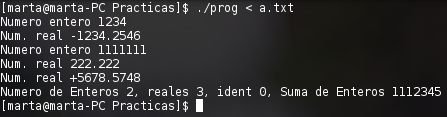
\includegraphics[width=0.5\textwidth]{1}
}
\qquad
\subfigure[Output del programa con el fichero c.txt] {
\label{tres}
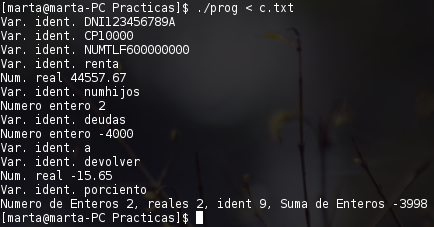
\includegraphics[width=0.5\textwidth]{3}
}
}
\caption{Output generados por los ficheros prueba}
\label{output}
\end{figure}

\subsection{\textcolor{p5}Creando nuestro propio fichero LeX}
Las semejanzas entre la sintaxis de LaTeX y la de HTML se observan en la \hyperref[latexhtml]{Tabla \ref*{latexhtml}}.

\begin{table}[H]
\centering
\begin{tabular}{| c | p{8cm} | p{4.5cm} |}
\hline
& LaTeX & HTML \\
\hline
\multirow{3}{*}{\textbf{Negrita}} & \mint{latex}|\textbf{texto}| & \mint{html}|<b>texto</b>| \\
\hline
\multirow{3}{*}{\textit{Cursiva}} & \mint{latex}|\textit{texto}| & \mint{html}|<i>texto</i>| \\
\hline
\multirow{3}{*}{\underline{Subrayado}} & \mint{latex}|\underline{texto}| & \mint{html}|<u>texto</u>| \\
\hline
\multirow{3}{*}{Capítulo} & \mint{latex}|\chapter{Nombre}| & \mint{html}|<h1>Nombre</h1>| \\
\hline
\multirow{3}{*}{Sección} & \mint{latex}|\section{Nombre}| & \mint{html}|<h2>Nombre</h2>| \\
\hline
\multirow{3}{*}{Subsección} & \mint{latex}|\subsection{Nombre}| & \mint{html}|<h3>Nombre</h3>| \\
\hline
\multirow{3}{*}{Subsubsección} & \mint{latex}|\subsubsection{Nombre}| & \mint{html}|<h4>Nombre</h4>| \\
\hline
\multirow{3}{*}{Descripción} & 
\begin{minted}{latex}
\begin{description}
\item[Nombre]
\end{description}
\end{minted}
 & \mint{html}|<h5>Nombre</h5>| \\
\hline
\multirow{3}{*}{Enlace} & \mint{latex}|\href{url}{texto}| & \mint{html}|<a href="url">texto</a>| \\
\hline
\multirow{3}{*}{imagen} & \mint{latex}|\includegraphics[width=1\textwidth]{imagen}| & \mint{html}|<img src="imagen.jpg"/>| \\
\hline
\multirow{3}{*}{Listar elementos} &
\begin{minted}{latex}
\begin{enumerate}
\item texto
\end{enumerate}
\end{minted}
&
\begin{minted}{html}
<ul>
  <li>texto</li>
</ul>
\end{minted}
\\
\hline
\end{tabular}

\caption{Semejanzas entre la sintaxis de HTML y la sintaxis de LaTeX}
\label{latexhtml}
\end{table}

A partir de esta tabla, definimos las expresiones regulares de un documento latex, tales como el texto en negrita. Así, al definir las reglas, definimos algo tal que ``cuando encuentres un \texttt{textbf} lo cambias por un \texttt{<b></b>}''.

A la hora de definir una imagen, como en LaTeX podemos incluir una imagen en el texto sin especificar su extensión y en HTML es obligatorio indicarla, debemos buscar el nombre del archivo completo en el sistema. También se ha decidido ignorar todos los \texttt{usepackage} de la cabecera por sencillez, excepto el que define que usaremos codificación UTF-8.

En HTML, cada párrafo va entre las etiquetas \texttt{<p></p>}, mientras que en LaTeX detecta los saltos de línea automáticamente. Por eso, debemos incluir una regla para añadir las etiquetas de párrafo. Aunque añade más etiquetas de la cuenta, tal y como se ve en la \hyperref[pruebahtml]{Figura \ref*{pruebahtml}}, se obtiene un resultado satisfactorio.

\begin{figure}[!h]
\centering
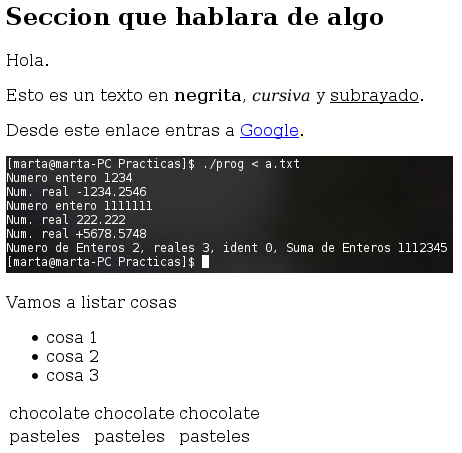
\includegraphics[width=0.7\textwidth]{prueba}
\caption{Vista en el navegador del fichero HTML generado}
\label{pruebahtml}
\end{figure}

Otro factor a tener en cuenta es el título, debe estar dentro del \texttt{<head>} en HTML, en LaTeX da igual si está en el preámbulo o en el cuerpo del documento, pero para que el conversor funcione correctamente, debe estar en el preámbulo.

Por último, también hay que tener en cuenta que un comentario en LaTeX se hace con el símbolo \%, por tanto, todas las cadenas que empiecen con el símbolo \% serán eliminadas.

El fichero LeX resultante es el siguiente:
\mylex[label={latex2html.lex}]{latex2html.lex}

\subsubsection{\textcolor{p5}Haciendo una pequeña prueba}
Vamos a generar el fichero HTML correspondiente al siguiente fichero LaTeX:

\mylatex[label={prueba\_conversor.tex}]{prueba_conversor.tex}

Tras ejecutar generar el programa con \texttt{lex} y compilarlo con \texttt{gcc}, ejecutamos el siguiente comando:
\begin{minted}[frame=single, label={prueba de nuestro conversor}]{bash}
./prog < prueba_conversor.tex > prueba_conver.html
\end{minted}

Y obtenemos el siguiente fichero HTML:
\myhtml[label={prueba\_conver.html}]{prueba_conver.html}

Este conversor lo he hecho junto a \textbf{Braulio Vargas López}.

\newpage
\thispagestyle{empty}
\ThisULCornerWallPaper{1}{p5.jpg}

\begin{tikzpicture}[remember picture,overlay]
\node [rectangle, rounded corners, fill=white, opacity=0.75, anchor=south west, minimum width=14cm, minimum height=5cm] (box) at (-1.5,-1.5) (box){}; % White rectangle - "minimum width/height" adjust the width and height of the box; "(-0.5,-10)" adjusts the position on the page
\node[anchor=west, xshift=-7cm, yshift=-3.2cm, text width=12cm] at (box.north){\chapter{\textcolor{p2}{Gramáticas regulares lineales por la derecha y por la izquierda}}};
\end{tikzpicture}\\[2.5cm]
\section{\textcolor{p2}Enunciado}
Sea $L = \{0u1~/~u\in\{0,1\}*\}$ obtener:
\begin{enumerate}[1.]
  \item Expresión regular
  \item A partir de la expresión regular, obtener el autómata finito determinítico.
  \item A partir del autómata finito determinístico, obtener:
  \begin{enumerate}[a)]
    \item Gramática regular lineal por la derecha
    \item Gramática regular lineal por la izquierda
  \end{enumerate}
\end{enumerate}

\section{\textcolor{p2}Solución}
\begin{enumerate}[1.]
\item Las cadenas que obtenemos con el lenguaje deben empezar con un símbolo terminal $0$ y acabar con un símbolo terminal $1$. Entre medias, puede haber una sucesión de símbolos terminales $0$ y símbolos terminales $1$  en orden completamente ``aleatorio''.

Por ejemplo, todas las siguientes cadenas pertenecerían al lenguaje:
\begin{enumerate}[\color{p2}{$\longrightarrow$}]
  \item $0011010110101011011$
  \item $01$
  \item $0101011001110000001$
  \item etc...
\end{enumerate}

Así, deducimos que la expresión regular del lenguaje sería la siguiente:
\begin{displaymath}
0(0+1)^*1
\end{displaymath}

\item La estructura de la expresión regular es muy simple, en primer lugar debe haber un símbolo terminal $0$, después tantos símbolos terminales $0$ como $1$ se quiera y finalmente un símbolo terminal $1$, por tanto, el autómata finito no determinístico que encaja sería el de la \hyperref[autonoder]{Figura \ref*{autonoder}}.

\begin{figure}[!h]
\centering
% Graphic for TeX using PGF
% Title: /home/marta/Documentos/Facultad/Tercero/MC/Practicas/Diagrama2.dia
% Creator: Dia v0.97.3
% CreationDate: Mon Nov  9 11:13:46 2015
% For: marta
% \usepackage{tikz}
% The following commands are not supported in PSTricks at present
% We define them conditionally, so when they are implemented,
% this pgf file will use them.
\ifx\du\undefined
  \newlength{\du}
\fi
\setlength{\du}{15\unitlength}
\begin{tikzpicture}
\pgftransformxscale{1.000000}
\pgftransformyscale{-1.000000}
\definecolor{dialinecolor}{rgb}{0.000000, 0.000000, 0.000000}
\pgfsetstrokecolor{dialinecolor}
\definecolor{dialinecolor}{rgb}{1.000000, 1.000000, 1.000000}
\pgfsetfillcolor{dialinecolor}
\definecolor{dialinecolor}{rgb}{1.000000, 1.000000, 1.000000}
\pgfsetfillcolor{dialinecolor}
\pgfpathellipse{\pgfpoint{5.074012\du}{5.153364\du}}{\pgfpoint{1.187397\du}{0\du}}{\pgfpoint{0\du}{1.064002\du}}
\pgfusepath{fill}
\pgfsetlinewidth{0.100000\du}
\pgfsetdash{}{0pt}
\pgfsetdash{}{0pt}
\pgfsetmiterjoin
\definecolor{dialinecolor}{rgb}{0.000000, 0.000000, 0.000000}
\pgfsetstrokecolor{dialinecolor}
\pgfpathellipse{\pgfpoint{5.074012\du}{5.153364\du}}{\pgfpoint{1.187397\du}{0\du}}{\pgfpoint{0\du}{1.064002\du}}
\pgfusepath{stroke}
% setfont left to latex
\definecolor{dialinecolor}{rgb}{0.000000, 0.000000, 0.000000}
\pgfsetstrokecolor{dialinecolor}
\node at (5.074012\du,5.348364\du){q0};
\definecolor{dialinecolor}{rgb}{1.000000, 1.000000, 1.000000}
\pgfsetfillcolor{dialinecolor}
\pgfpathellipse{\pgfpoint{10.197397\du}{5.119002\du}}{\pgfpoint{1.187397\du}{0\du}}{\pgfpoint{0\du}{1.064002\du}}
\pgfusepath{fill}
\pgfsetlinewidth{0.100000\du}
\pgfsetdash{}{0pt}
\pgfsetdash{}{0pt}
\pgfsetmiterjoin
\definecolor{dialinecolor}{rgb}{0.000000, 0.000000, 0.000000}
\pgfsetstrokecolor{dialinecolor}
\pgfpathellipse{\pgfpoint{10.197397\du}{5.119002\du}}{\pgfpoint{1.187397\du}{0\du}}{\pgfpoint{0\du}{1.064002\du}}
\pgfusepath{stroke}
% setfont left to latex
\definecolor{dialinecolor}{rgb}{0.000000, 0.000000, 0.000000}
\pgfsetstrokecolor{dialinecolor}
\node at (10.197397\du,5.314002\du){q1};
\definecolor{dialinecolor}{rgb}{1.000000, 1.000000, 1.000000}
\pgfsetfillcolor{dialinecolor}
\pgfpathellipse{\pgfpoint{15.660000\du}{5.205000\du}}{\pgfpoint{1.390000\du}{0\du}}{\pgfpoint{0\du}{1.345000\du}}
\pgfusepath{fill}
\pgfsetlinewidth{0.100000\du}
\pgfsetdash{}{0pt}
\pgfsetdash{}{0pt}
\pgfsetmiterjoin
\definecolor{dialinecolor}{rgb}{0.000000, 0.000000, 0.000000}
\pgfsetstrokecolor{dialinecolor}
\pgfpathellipse{\pgfpoint{15.660000\du}{5.205000\du}}{\pgfpoint{1.390000\du}{0\du}}{\pgfpoint{0\du}{1.345000\du}}
\pgfusepath{stroke}
% setfont left to latex
\definecolor{dialinecolor}{rgb}{0.000000, 0.000000, 0.000000}
\pgfsetstrokecolor{dialinecolor}
\node at (15.660000\du,5.400000\du){q2};
\pgfsetlinewidth{0.100000\du}
\pgfsetdash{}{0pt}
\pgfsetdash{}{0pt}
\pgfsetbuttcap
{
\definecolor{dialinecolor}{rgb}{0.000000, 0.000000, 0.000000}
\pgfsetfillcolor{dialinecolor}
% was here!!!
\pgfsetarrowsend{stealth}
\definecolor{dialinecolor}{rgb}{0.000000, 0.000000, 0.000000}
\pgfsetstrokecolor{dialinecolor}
\draw (1.950000\du,5.100000\du)--(3.886615\du,5.153364\du);
}
\pgfsetlinewidth{0.100000\du}
\pgfsetdash{}{0pt}
\pgfsetdash{}{0pt}
\pgfsetbuttcap
{
\definecolor{dialinecolor}{rgb}{0.000000, 0.000000, 0.000000}
\pgfsetfillcolor{dialinecolor}
% was here!!!
\pgfsetarrowsend{stealth}
\definecolor{dialinecolor}{rgb}{0.000000, 0.000000, 0.000000}
\pgfsetstrokecolor{dialinecolor}
\draw (6.307852\du,5.142592\du)--(9.010000\du,5.119002\du);
}
\pgfsetlinewidth{0.100000\du}
\pgfsetdash{}{0pt}
\pgfsetdash{}{0pt}
\pgfsetbuttcap
{
\definecolor{dialinecolor}{rgb}{0.000000, 0.000000, 0.000000}
\pgfsetfillcolor{dialinecolor}
% was here!!!
\pgfsetarrowsend{stealth}
\definecolor{dialinecolor}{rgb}{0.000000, 0.000000, 0.000000}
\pgfsetstrokecolor{dialinecolor}
\draw (11.413680\du,5.138150\du)--(14.225000\du,5.182409\du);
}
% setfont left to latex
\definecolor{dialinecolor}{rgb}{0.000000, 0.000000, 0.000000}
\pgfsetstrokecolor{dialinecolor}
\node[anchor=west] at (7.200000\du,4.450000\du){0};
% setfont left to latex
\definecolor{dialinecolor}{rgb}{0.000000, 0.000000, 0.000000}
\pgfsetstrokecolor{dialinecolor}
\node[anchor=west] at (12.450000\du,4.600000\du){1};
\pgfsetlinewidth{0.100000\du}
\pgfsetdash{}{0pt}
\pgfsetdash{}{0pt}
\pgfsetbuttcap
{
\definecolor{dialinecolor}{rgb}{0.000000, 0.000000, 0.000000}
\pgfsetfillcolor{dialinecolor}
% was here!!!
\pgfsetarrowsend{stealth}
\definecolor{dialinecolor}{rgb}{0.000000, 0.000000, 0.000000}
\pgfsetstrokecolor{dialinecolor}
\pgfpathmoveto{\pgfpoint{10.651730\du}{4.136032\du}}
\pgfpatharc{59}{-238}{0.858090\du and 0.858090\du}
\pgfusepath{stroke}
}
% setfont left to latex
\definecolor{dialinecolor}{rgb}{0.000000, 0.000000, 0.000000}
\pgfsetstrokecolor{dialinecolor}
\node[anchor=west] at (9.850000\du,2.250000\du){0,1};
\definecolor{dialinecolor}{rgb}{1.000000, 1.000000, 1.000000}
\pgfsetfillcolor{dialinecolor}
\pgfpathellipse{\pgfpoint{15.676941\du}{5.198331\du}}{\pgfpoint{1.173059\du}{0\du}}{\pgfpoint{0\du}{1.151669\du}}
\pgfusepath{fill}
\pgfsetlinewidth{0.100000\du}
\pgfsetdash{}{0pt}
\pgfsetdash{}{0pt}
\pgfsetmiterjoin
\definecolor{dialinecolor}{rgb}{0.000000, 0.000000, 0.000000}
\pgfsetstrokecolor{dialinecolor}
\pgfpathellipse{\pgfpoint{15.676941\du}{5.198331\du}}{\pgfpoint{1.173059\du}{0\du}}{\pgfpoint{0\du}{1.151669\du}}
\pgfusepath{stroke}
% setfont left to latex
\definecolor{dialinecolor}{rgb}{0.000000, 0.000000, 0.000000}
\pgfsetstrokecolor{dialinecolor}
\node at (15.676941\du,5.393331\du){q2};
\end{tikzpicture}

\caption{Autómata finito no determinístico correspondiente a la expresión regular calculada en el apartado anterior}
\label{autonoder}
\end{figure}

El autómata finito determinístico correspondiente, debe tener un \textit{\textcolor{p2}{estado de error}} al que van todas las transiciones no definidas en los otros estados. Sería el de la \hyperref[autoder]{Figura \ref*{autoder}}.

\begin{figure}[!h]
\centering
% Graphic for TeX using PGF
% Title: /home/marta/Documentos/Facultad/Tercero/MC/Practicas/Diagrama1.dia
% Creator: Dia v0.97.3
% CreationDate: Mon Nov  9 11:09:00 2015
% For: marta
% \usepackage{tikz}
% The following commands are not supported in PSTricks at present
% We define them conditionally, so when they are implemented,
% this pgf file will use them.
\ifx\du\undefined
  \newlength{\du}
\fi
\setlength{\du}{15\unitlength}
\begin{tikzpicture}
\pgftransformxscale{1.000000}
\pgftransformyscale{-1.000000}
\definecolor{dialinecolor}{rgb}{0.000000, 0.000000, 0.000000}
\pgfsetstrokecolor{dialinecolor}
\definecolor{dialinecolor}{rgb}{1.000000, 1.000000, 1.000000}
\pgfsetfillcolor{dialinecolor}
\definecolor{dialinecolor}{rgb}{1.000000, 1.000000, 1.000000}
\pgfsetfillcolor{dialinecolor}
\pgfpathellipse{\pgfpoint{7.051127\du}{6.464277\du}}{\pgfpoint{1.155021\du}{0\du}}{\pgfpoint{0\du}{1.089380\du}}
\pgfusepath{fill}
\pgfsetlinewidth{0.100000\du}
\pgfsetdash{}{0pt}
\pgfsetdash{}{0pt}
\pgfsetmiterjoin
\definecolor{dialinecolor}{rgb}{0.000000, 0.000000, 0.000000}
\pgfsetstrokecolor{dialinecolor}
\pgfpathellipse{\pgfpoint{7.051127\du}{6.464277\du}}{\pgfpoint{1.155021\du}{0\du}}{\pgfpoint{0\du}{1.089380\du}}
\pgfusepath{stroke}
% setfont left to latex
\definecolor{dialinecolor}{rgb}{0.000000, 0.000000, 0.000000}
\pgfsetstrokecolor{dialinecolor}
\node at (7.051127\du,6.659277\du){q0};
\definecolor{dialinecolor}{rgb}{1.000000, 1.000000, 1.000000}
\pgfsetfillcolor{dialinecolor}
\pgfpathellipse{\pgfpoint{12.315021\du}{6.444380\du}}{\pgfpoint{1.155021\du}{0\du}}{\pgfpoint{0\du}{1.089380\du}}
\pgfusepath{fill}
\pgfsetlinewidth{0.100000\du}
\pgfsetdash{}{0pt}
\pgfsetdash{}{0pt}
\pgfsetmiterjoin
\definecolor{dialinecolor}{rgb}{0.000000, 0.000000, 0.000000}
\pgfsetstrokecolor{dialinecolor}
\pgfpathellipse{\pgfpoint{12.315021\du}{6.444380\du}}{\pgfpoint{1.155021\du}{0\du}}{\pgfpoint{0\du}{1.089380\du}}
\pgfusepath{stroke}
% setfont left to latex
\definecolor{dialinecolor}{rgb}{0.000000, 0.000000, 0.000000}
\pgfsetstrokecolor{dialinecolor}
\node at (12.315021\du,6.639380\du){q1};
\definecolor{dialinecolor}{rgb}{1.000000, 1.000000, 1.000000}
\pgfsetfillcolor{dialinecolor}
\pgfpathellipse{\pgfpoint{18.425000\du}{6.500000\du}}{\pgfpoint{2.675000\du}{0\du}}{\pgfpoint{0\du}{1.450000\du}}
\pgfusepath{fill}
\pgfsetlinewidth{0.100000\du}
\pgfsetdash{}{0pt}
\pgfsetdash{}{0pt}
\pgfsetmiterjoin
\definecolor{dialinecolor}{rgb}{0.000000, 0.000000, 0.000000}
\pgfsetstrokecolor{dialinecolor}
\pgfpathellipse{\pgfpoint{18.425000\du}{6.500000\du}}{\pgfpoint{2.675000\du}{0\du}}{\pgfpoint{0\du}{1.450000\du}}
\pgfusepath{stroke}
% setfont left to latex
\definecolor{dialinecolor}{rgb}{0.000000, 0.000000, 0.000000}
\pgfsetstrokecolor{dialinecolor}
\node at (18.425000\du,6.695000\du){};
\definecolor{dialinecolor}{rgb}{1.000000, 1.000000, 1.000000}
\pgfsetfillcolor{dialinecolor}
\pgfpathellipse{\pgfpoint{18.395021\du}{6.553385\du}}{\pgfpoint{2.331550\du}{0\du}}{\pgfpoint{0\du}{1.148919\du}}
\pgfusepath{fill}
\pgfsetlinewidth{0.100000\du}
\pgfsetdash{}{0pt}
\pgfsetdash{}{0pt}
\pgfsetmiterjoin
\definecolor{dialinecolor}{rgb}{0.000000, 0.000000, 0.000000}
\pgfsetstrokecolor{dialinecolor}
\pgfpathellipse{\pgfpoint{18.395021\du}{6.553385\du}}{\pgfpoint{2.331550\du}{0\du}}{\pgfpoint{0\du}{1.148919\du}}
\pgfusepath{stroke}
% setfont left to latex
\definecolor{dialinecolor}{rgb}{0.000000, 0.000000, 0.000000}
\pgfsetstrokecolor{dialinecolor}
\node at (18.395021\du,6.748385\du){\{q1,q2\}};
\pgfsetlinewidth{0.100000\du}
\pgfsetdash{}{0pt}
\pgfsetdash{}{0pt}
\pgfsetbuttcap
{
\definecolor{dialinecolor}{rgb}{0.000000, 0.000000, 0.000000}
\pgfsetfillcolor{dialinecolor}
% was here!!!
\pgfsetarrowsend{stealth}
\definecolor{dialinecolor}{rgb}{0.000000, 0.000000, 0.000000}
\pgfsetstrokecolor{dialinecolor}
\draw (8.206148\du,6.464277\du)--(11.110247\du,6.450214\du);
}
\pgfsetlinewidth{0.100000\du}
\pgfsetdash{}{0pt}
\pgfsetdash{}{0pt}
\pgfsetbuttcap
{
\definecolor{dialinecolor}{rgb}{0.000000, 0.000000, 0.000000}
\pgfsetfillcolor{dialinecolor}
% was here!!!
\pgfsetarrowsend{stealth}
\definecolor{dialinecolor}{rgb}{0.000000, 0.000000, 0.000000}
\pgfsetstrokecolor{dialinecolor}
\draw (4.200000\du,6.550000\du)--(5.896105\du,6.464277\du);
}
\pgfsetlinewidth{0.100000\du}
\pgfsetdash{}{0pt}
\pgfsetdash{}{0pt}
\pgfsetbuttcap
{
\definecolor{dialinecolor}{rgb}{0.000000, 0.000000, 0.000000}
\pgfsetfillcolor{dialinecolor}
% was here!!!
\pgfsetarrowsend{stealth}
\definecolor{dialinecolor}{rgb}{0.000000, 0.000000, 0.000000}
\pgfsetstrokecolor{dialinecolor}
\draw (13.470043\du,6.444380\du)--(15.750000\du,6.500000\du);
}
\definecolor{dialinecolor}{rgb}{1.000000, 1.000000, 1.000000}
\pgfsetfillcolor{dialinecolor}
\pgfpathellipse{\pgfpoint{9.565021\du}{10.044380\du}}{\pgfpoint{1.155021\du}{0\du}}{\pgfpoint{0\du}{1.089380\du}}
\pgfusepath{fill}
\pgfsetlinewidth{0.100000\du}
\pgfsetdash{}{0pt}
\pgfsetdash{}{0pt}
\pgfsetmiterjoin
\definecolor{dialinecolor}{rgb}{0.000000, 0.000000, 0.000000}
\pgfsetstrokecolor{dialinecolor}
\pgfpathellipse{\pgfpoint{9.565021\du}{10.044380\du}}{\pgfpoint{1.155021\du}{0\du}}{\pgfpoint{0\du}{1.089380\du}}
\pgfusepath{stroke}
% setfont left to latex
\definecolor{dialinecolor}{rgb}{0.000000, 0.000000, 0.000000}
\pgfsetstrokecolor{dialinecolor}
\node at (9.565021\du,10.239380\du){$\emptyset$};
\pgfsetlinewidth{0.100000\du}
\pgfsetdash{}{0pt}
\pgfsetdash{}{0pt}
\pgfsetbuttcap
{
\definecolor{dialinecolor}{rgb}{0.000000, 0.000000, 0.000000}
\pgfsetfillcolor{dialinecolor}
% was here!!!
\pgfsetarrowsend{stealth}
\definecolor{dialinecolor}{rgb}{0.000000, 0.000000, 0.000000}
\pgfsetstrokecolor{dialinecolor}
\draw (7.717039\du,7.412620\du)--(8.899109\du,9.096037\du);
}
\pgfsetlinewidth{0.100000\du}
\pgfsetdash{}{0pt}
\pgfsetdash{}{0pt}
\pgfsetbuttcap
{
\definecolor{dialinecolor}{rgb}{0.000000, 0.000000, 0.000000}
\pgfsetfillcolor{dialinecolor}
% was here!!!
\pgfsetarrowsend{stealth}
\definecolor{dialinecolor}{rgb}{0.000000, 0.000000, 0.000000}
\pgfsetstrokecolor{dialinecolor}
\pgfpathmoveto{\pgfpoint{12.756958\du}{5.437963\du}}
\pgfpatharc{62}{-241}{0.925170\du and 0.925170\du}
\pgfusepath{stroke}
}
\pgfsetlinewidth{0.100000\du}
\pgfsetdash{}{0pt}
\pgfsetdash{}{0pt}
\pgfsetbuttcap
{
\definecolor{dialinecolor}{rgb}{0.000000, 0.000000, 0.000000}
\pgfsetfillcolor{dialinecolor}
% was here!!!
\pgfsetarrowsend{stealth}
\definecolor{dialinecolor}{rgb}{0.000000, 0.000000, 0.000000}
\pgfsetstrokecolor{dialinecolor}
\pgfpathmoveto{\pgfpoint{18.424947\du}{5.050053\du}}
\pgfpatharc{45}{-237}{0.817306\du and 0.817306\du}
\pgfusepath{stroke}
}
\pgfsetlinewidth{0.100000\du}
\pgfsetdash{}{0pt}
\pgfsetdash{}{0pt}
\pgfsetbuttcap
{
\definecolor{dialinecolor}{rgb}{0.000000, 0.000000, 0.000000}
\pgfsetfillcolor{dialinecolor}
% was here!!!
\pgfsetarrowsend{stealth}
\definecolor{dialinecolor}{rgb}{0.000000, 0.000000, 0.000000}
\pgfsetstrokecolor{dialinecolor}
\pgfpathmoveto{\pgfpoint{10.007021\du}{11.050788\du}}
\pgfpatharc{171}{-99}{0.873232\du and 0.873232\du}
\pgfusepath{stroke}
}
% setfont left to latex
\definecolor{dialinecolor}{rgb}{0.000000, 0.000000, 0.000000}
\pgfsetstrokecolor{dialinecolor}
\node[anchor=west] at (9.050000\du,5.700000\du){0};
% setfont left to latex
\definecolor{dialinecolor}{rgb}{0.000000, 0.000000, 0.000000}
\pgfsetstrokecolor{dialinecolor}
\node[anchor=west] at (8.600000\du,7.850000\du){1};
% setfont left to latex
\definecolor{dialinecolor}{rgb}{0.000000, 0.000000, 0.000000}
\pgfsetstrokecolor{dialinecolor}
\node[anchor=west] at (12.100000\du,10.900000\du){0,1};
% setfont left to latex
\definecolor{dialinecolor}{rgb}{0.000000, 0.000000, 0.000000}
\pgfsetstrokecolor{dialinecolor}
\node[anchor=west] at (12.000000\du,3.200000\du){0};
% setfont left to latex
\definecolor{dialinecolor}{rgb}{0.000000, 0.000000, 0.000000}
\pgfsetstrokecolor{dialinecolor}
\node[anchor=west] at (14.150000\du,6.000000\du){1};
% setfont left to latex
\definecolor{dialinecolor}{rgb}{0.000000, 0.000000, 0.000000}
\pgfsetstrokecolor{dialinecolor}
\node[anchor=west] at (17.650000\du,3.300000\du){1};
\pgfsetlinewidth{0.100000\du}
\pgfsetdash{}{0pt}
\pgfsetdash{}{0pt}
\pgfsetmiterjoin
\pgfsetbuttcap
{
\definecolor{dialinecolor}{rgb}{0.000000, 0.000000, 0.000000}
\pgfsetfillcolor{dialinecolor}
% was here!!!
\pgfsetarrowsend{stealth}
\definecolor{dialinecolor}{rgb}{0.000000, 0.000000, 0.000000}
\pgfsetstrokecolor{dialinecolor}
\pgfpathmoveto{\pgfpoint{17.483211\du}{7.903450\du}}
\pgfpathcurveto{\pgfpoint{16.208211\du}{9.803450\du}}{\pgfpoint{14.475866\du}{10.201192\du}}{\pgfpoint{12.890887\du}{7.445572\du}}
\pgfusepath{stroke}
}
% setfont left to latex
\definecolor{dialinecolor}{rgb}{0.000000, 0.000000, 0.000000}
\pgfsetstrokecolor{dialinecolor}
\node[anchor=west] at (14.900000\du,10.400000\du){0};
\end{tikzpicture}

\caption{Autómata finito determinístico correspondiente al no determinístico calculado}
\label{autoder}
\end{figure}

\newpage
\item ~
\begin{enumerate}[a)]
\item Las gramáticas regulares lineales por la derecha son de la forma:
\begin{displaymath}
A \rightarrow uB, \qquad\ A \rightarrow u
\end{displaymath}

donde $u$ es una secuencia de símbolos terminales del lenguaje y $B$, una variable.

Teniendo en cuenta esta estructura y el autómata finito no determinista obtenido en el apartado anterior (\hyperref[autoder]{Figura \ref*{autoder}}), la gramática lineal por la derecha correspondiente sería:
\begin{displaymath}
q_0 \rightarrow 0q_1, \qquad\ q_0 \rightarrow 1\emptyset, \qquad\ q_1 \rightarrow 0q_1, \qquad\ q_1 \rightarrow 1\{q_1,q_2\},
\end{displaymath}
\begin{displaymath}
\{q_1,q_2\} \rightarrow 1\{q_1,q_2\}, \qquad\ \{q_1,q_2\} \rightarrow 0q_1, \qquad\ \emptyset \rightarrow 0\emptyset, \qquad\ \emptyset \rightarrow 1\emptyset
\end{displaymath}

\item En el caso de las gramáticas regulares lineales por la izquierda, tienen la siguiente estructura:
\begin{displaymath}
A \rightarrow Bu, \qquad\ A \rightarrow u
\end{displaymath}

donde $u$ es una secuencia de símbolos terminales del lenguaje y $B$, una variable.

Pero para llegar a la gramática a partir del autómata, debemos invertirlo\footnote{Invertir un autómata significa invertir el sentido de las fechas y hacer autómata inicial al final y final al inicial} primero. El resultado de invertir el autómata se ve en la \hyperref[invertido]{Figura \ref*{invertido}}. 

\begin{figure}[!h]
\centering
% Graphic for TeX using PGF
% Title: /home/marta/Documentos/Facultad/Tercero/MC/Practicas/Diagrama3.dia
% Creator: Dia v0.97.3
% CreationDate: Mon Nov  9 11:20:34 2015
% For: marta
% \usepackage{tikz}
% The following commands are not supported in PSTricks at present
% We define them conditionally, so when they are implemented,
% this pgf file will use them.
\ifx\du\undefined
  \newlength{\du}
\fi
\setlength{\du}{15\unitlength}
\begin{tikzpicture}
\pgftransformxscale{1.000000}
\pgftransformyscale{-1.000000}
\definecolor{dialinecolor}{rgb}{0.000000, 0.000000, 0.000000}
\pgfsetstrokecolor{dialinecolor}
\definecolor{dialinecolor}{rgb}{1.000000, 1.000000, 1.000000}
\pgfsetfillcolor{dialinecolor}
\definecolor{dialinecolor}{rgb}{1.000000, 1.000000, 1.000000}
\pgfsetfillcolor{dialinecolor}
\pgfpathellipse{\pgfpoint{4.866804\du}{6.251828\du}}{\pgfpoint{1.566804\du}{0\du}}{\pgfpoint{0\du}{1.451828\du}}
\pgfusepath{fill}
\pgfsetlinewidth{0.100000\du}
\pgfsetdash{}{0pt}
\pgfsetdash{}{0pt}
\pgfsetmiterjoin
\definecolor{dialinecolor}{rgb}{0.000000, 0.000000, 0.000000}
\pgfsetstrokecolor{dialinecolor}
\pgfpathellipse{\pgfpoint{4.866804\du}{6.251828\du}}{\pgfpoint{1.566804\du}{0\du}}{\pgfpoint{0\du}{1.451828\du}}
\pgfusepath{stroke}
% setfont left to latex
\definecolor{dialinecolor}{rgb}{0.000000, 0.000000, 0.000000}
\pgfsetstrokecolor{dialinecolor}
\node at (4.866804\du,6.446828\du){q0};
\definecolor{dialinecolor}{rgb}{1.000000, 1.000000, 1.000000}
\pgfsetfillcolor{dialinecolor}
\pgfpathellipse{\pgfpoint{10.542481\du}{6.594380\du}}{\pgfpoint{1.155021\du}{0\du}}{\pgfpoint{0\du}{1.089380\du}}
\pgfusepath{fill}
\pgfsetlinewidth{0.100000\du}
\pgfsetdash{}{0pt}
\pgfsetdash{}{0pt}
\pgfsetmiterjoin
\definecolor{dialinecolor}{rgb}{0.000000, 0.000000, 0.000000}
\pgfsetstrokecolor{dialinecolor}
\pgfpathellipse{\pgfpoint{10.542481\du}{6.594380\du}}{\pgfpoint{1.155021\du}{0\du}}{\pgfpoint{0\du}{1.089380\du}}
\pgfusepath{stroke}
% setfont left to latex
\definecolor{dialinecolor}{rgb}{0.000000, 0.000000, 0.000000}
\pgfsetstrokecolor{dialinecolor}
\node at (10.542481\du,6.789380\du){q1};
\definecolor{dialinecolor}{rgb}{1.000000, 1.000000, 1.000000}
\pgfsetfillcolor{dialinecolor}
\pgfpathellipse{\pgfpoint{16.622481\du}{6.653385\du}}{\pgfpoint{2.331550\du}{0\du}}{\pgfpoint{0\du}{1.148919\du}}
\pgfusepath{fill}
\pgfsetlinewidth{0.100000\du}
\pgfsetdash{}{0pt}
\pgfsetdash{}{0pt}
\pgfsetmiterjoin
\definecolor{dialinecolor}{rgb}{0.000000, 0.000000, 0.000000}
\pgfsetstrokecolor{dialinecolor}
\pgfpathellipse{\pgfpoint{16.622481\du}{6.653385\du}}{\pgfpoint{2.331550\du}{0\du}}{\pgfpoint{0\du}{1.148919\du}}
\pgfusepath{stroke}
% setfont left to latex
\definecolor{dialinecolor}{rgb}{0.000000, 0.000000, 0.000000}
\pgfsetstrokecolor{dialinecolor}
\node at (16.622481\du,6.848385\du){\{q1,q2\}};
\definecolor{dialinecolor}{rgb}{1.000000, 1.000000, 1.000000}
\pgfsetfillcolor{dialinecolor}
\pgfpathellipse{\pgfpoint{7.792481\du}{10.194380\du}}{\pgfpoint{1.155021\du}{0\du}}{\pgfpoint{0\du}{1.089380\du}}
\pgfusepath{fill}
\pgfsetlinewidth{0.100000\du}
\pgfsetdash{}{0pt}
\pgfsetdash{}{0pt}
\pgfsetmiterjoin
\definecolor{dialinecolor}{rgb}{0.000000, 0.000000, 0.000000}
\pgfsetstrokecolor{dialinecolor}
\pgfpathellipse{\pgfpoint{7.792481\du}{10.194380\du}}{\pgfpoint{1.155021\du}{0\du}}{\pgfpoint{0\du}{1.089380\du}}
\pgfusepath{stroke}
% setfont left to latex
\definecolor{dialinecolor}{rgb}{0.000000, 0.000000, 0.000000}
\pgfsetstrokecolor{dialinecolor}
\node at (7.792481\du,10.389380\du){$\emptyset$};
\pgfsetlinewidth{0.100000\du}
\pgfsetdash{}{0pt}
\pgfsetdash{}{0pt}
\pgfsetbuttcap
{
\definecolor{dialinecolor}{rgb}{0.000000, 0.000000, 0.000000}
\pgfsetfillcolor{dialinecolor}
% was here!!!
\pgfsetarrowsend{stealth}
\definecolor{dialinecolor}{rgb}{0.000000, 0.000000, 0.000000}
\pgfsetstrokecolor{dialinecolor}
\pgfpathmoveto{\pgfpoint{10.984418\du}{5.587963\du}}
\pgfpatharc{62}{-241}{0.925170\du and 0.925170\du}
\pgfusepath{stroke}
}
\pgfsetlinewidth{0.100000\du}
\pgfsetdash{}{0pt}
\pgfsetdash{}{0pt}
\pgfsetbuttcap
{
\definecolor{dialinecolor}{rgb}{0.000000, 0.000000, 0.000000}
\pgfsetfillcolor{dialinecolor}
% was here!!!
\pgfsetarrowsend{stealth}
\definecolor{dialinecolor}{rgb}{0.000000, 0.000000, 0.000000}
\pgfsetstrokecolor{dialinecolor}
\pgfpathmoveto{\pgfpoint{17.514666\du}{5.591956\du}}
\pgfpatharc{62}{-230}{0.795239\du and 0.795239\du}
\pgfusepath{stroke}
}
\pgfsetlinewidth{0.100000\du}
\pgfsetdash{}{0pt}
\pgfsetdash{}{0pt}
\pgfsetbuttcap
{
\definecolor{dialinecolor}{rgb}{0.000000, 0.000000, 0.000000}
\pgfsetfillcolor{dialinecolor}
% was here!!!
\pgfsetarrowsend{stealth}
\definecolor{dialinecolor}{rgb}{0.000000, 0.000000, 0.000000}
\pgfsetstrokecolor{dialinecolor}
\pgfpathmoveto{\pgfpoint{8.234481\du}{11.200788\du}}
\pgfpatharc{171}{-99}{0.873232\du and 0.873232\du}
\pgfusepath{stroke}
}
% setfont left to latex
\definecolor{dialinecolor}{rgb}{0.000000, 0.000000, 0.000000}
\pgfsetstrokecolor{dialinecolor}
\node[anchor=west] at (7.927460\du,6.400000\du){0};
% setfont left to latex
\definecolor{dialinecolor}{rgb}{0.000000, 0.000000, 0.000000}
\pgfsetstrokecolor{dialinecolor}
\node[anchor=west] at (6.727460\du,8.600000\du){1};
% setfont left to latex
\definecolor{dialinecolor}{rgb}{0.000000, 0.000000, 0.000000}
\pgfsetstrokecolor{dialinecolor}
\node[anchor=west] at (10.327460\du,11.050000\du){0,1};
% setfont left to latex
\definecolor{dialinecolor}{rgb}{0.000000, 0.000000, 0.000000}
\pgfsetstrokecolor{dialinecolor}
\node[anchor=west] at (10.227460\du,3.350000\du){0};
% setfont left to latex
\definecolor{dialinecolor}{rgb}{0.000000, 0.000000, 0.000000}
\pgfsetstrokecolor{dialinecolor}
\node[anchor=west] at (12.377460\du,6.150000\du){1};
% setfont left to latex
\definecolor{dialinecolor}{rgb}{0.000000, 0.000000, 0.000000}
\pgfsetstrokecolor{dialinecolor}
\node[anchor=west] at (16.477460\du,3.850000\du){1};
% setfont left to latex
\definecolor{dialinecolor}{rgb}{0.000000, 0.000000, 0.000000}
\pgfsetstrokecolor{dialinecolor}
\node[anchor=west] at (13.127460\du,10.250000\du){0};
\pgfsetlinewidth{0.100000\du}
\pgfsetdash{}{0pt}
\pgfsetdash{}{0pt}
\pgfsetbuttcap
{
\definecolor{dialinecolor}{rgb}{0.000000, 0.000000, 0.000000}
\pgfsetfillcolor{dialinecolor}
% was here!!!
\pgfsetarrowsend{stealth}
\definecolor{dialinecolor}{rgb}{0.000000, 0.000000, 0.000000}
\pgfsetstrokecolor{dialinecolor}
\draw (14.290931\du,6.653385\du)--(11.697503\du,6.594380\du);
}
\pgfsetlinewidth{0.100000\du}
\pgfsetdash{}{0pt}
\pgfsetdash{}{0pt}
\pgfsetbuttcap
{
\definecolor{dialinecolor}{rgb}{0.000000, 0.000000, 0.000000}
\pgfsetfillcolor{dialinecolor}
% was here!!!
\pgfsetarrowsend{stealth}
\definecolor{dialinecolor}{rgb}{0.000000, 0.000000, 0.000000}
\pgfsetstrokecolor{dialinecolor}
\draw (20.450000\du,6.600000\du)--(19.001598\du,6.620202\du);
}
\pgfsetlinewidth{0.100000\du}
\pgfsetdash{}{0pt}
\pgfsetdash{}{0pt}
\pgfsetmiterjoin
\pgfsetbuttcap
{
\definecolor{dialinecolor}{rgb}{0.000000, 0.000000, 0.000000}
\pgfsetfillcolor{dialinecolor}
% was here!!!
\pgfsetarrowsend{stealth}
\definecolor{dialinecolor}{rgb}{0.000000, 0.000000, 0.000000}
\pgfsetstrokecolor{dialinecolor}
\pgfpathmoveto{\pgfpoint{11.162314\du}{7.568852\du}}
\pgfpathcurveto{\pgfpoint{12.469833\du}{9.624473\du}}{\pgfpoint{13.569168\du}{10.036906\du}}{\pgfpoint{15.641650\du}{7.740291\du}}
\pgfusepath{stroke}
}
\pgfsetlinewidth{0.100000\du}
\pgfsetdash{}{0pt}
\pgfsetdash{}{0pt}
\pgfsetbuttcap
{
\definecolor{dialinecolor}{rgb}{0.000000, 0.000000, 0.000000}
\pgfsetfillcolor{dialinecolor}
% was here!!!
\pgfsetarrowsend{stealth}
\definecolor{dialinecolor}{rgb}{0.000000, 0.000000, 0.000000}
\pgfsetstrokecolor{dialinecolor}
\draw (6.975758\du,9.424072\du)--(5.466394\du,7.593143\du);
}
\definecolor{dialinecolor}{rgb}{1.000000, 1.000000, 1.000000}
\pgfsetfillcolor{dialinecolor}
\pgfpathellipse{\pgfpoint{4.875000\du}{6.274433\du}}{\pgfpoint{1.225000\du}{0\du}}{\pgfpoint{0\du}{1.169558\du}}
\pgfusepath{fill}
\pgfsetlinewidth{0.100000\du}
\pgfsetdash{}{0pt}
\pgfsetdash{}{0pt}
\pgfsetmiterjoin
\definecolor{dialinecolor}{rgb}{0.000000, 0.000000, 0.000000}
\pgfsetstrokecolor{dialinecolor}
\pgfpathellipse{\pgfpoint{4.875000\du}{6.274433\du}}{\pgfpoint{1.225000\du}{0\du}}{\pgfpoint{0\du}{1.169558\du}}
\pgfusepath{stroke}
% setfont left to latex
\definecolor{dialinecolor}{rgb}{0.000000, 0.000000, 0.000000}
\pgfsetstrokecolor{dialinecolor}
\node at (4.875000\du,6.469433\du){q0};
\pgfsetlinewidth{0.100000\du}
\pgfsetdash{}{0pt}
\pgfsetdash{}{0pt}
\pgfsetbuttcap
{
\definecolor{dialinecolor}{rgb}{0.000000, 0.000000, 0.000000}
\pgfsetfillcolor{dialinecolor}
% was here!!!
\pgfsetarrowsend{stealth}
\definecolor{dialinecolor}{rgb}{0.000000, 0.000000, 0.000000}
\pgfsetstrokecolor{dialinecolor}
\draw (9.387460\du,6.594380\du)--(6.314342\du,6.807419\du);
}
\end{tikzpicture}

\caption{Autómata finito no determinístico invertido}
\label{invertido}
\end{figure}

Sin embargo, el autómata de la \hyperref[invertido]{Figura \ref*{invertido}}, no es determinístico por lo que antes de pasar a obtener la gramática regular lineal por la izquierda debemos pasarlo a determinístico. El resultado de ésto es la \hyperref[inverder]{Figura \ref*{inverder}}.

\begin{figure}
\centering
% Graphic for TeX using PGF
% Title: /home/marta/Documentos/Facultad/Tercero/MC/Practicas/Diagrama5.dia
% Creator: Dia v0.97.3
% CreationDate: Mon Nov  9 11:52:21 2015
% For: marta
% \usepackage{tikz}
% The following commands are not supported in PSTricks at present
% We define them conditionally, so when they are implemented,
% this pgf file will use them.
\ifx\du\undefined
  \newlength{\du}
\fi
\setlength{\du}{15\unitlength}
\begin{tikzpicture}
\pgftransformxscale{1.000000}
\pgftransformyscale{-1.000000}
\definecolor{dialinecolor}{rgb}{0.000000, 0.000000, 0.000000}
\pgfsetstrokecolor{dialinecolor}
\definecolor{dialinecolor}{rgb}{1.000000, 1.000000, 1.000000}
\pgfsetfillcolor{dialinecolor}
% setfont left to latex
\definecolor{dialinecolor}{rgb}{0.000000, 0.000000, 0.000000}
\pgfsetstrokecolor{dialinecolor}
\node[anchor=west] at (1.550000\du,1.400000\du){Tomando q3 como \{q1,q2\}};
\definecolor{dialinecolor}{rgb}{1.000000, 1.000000, 1.000000}
\pgfsetfillcolor{dialinecolor}
\pgfpathellipse{\pgfpoint{4.971110\du}{4.953364\du}}{\pgfpoint{1.134495\du}{0\du}}{\pgfpoint{0\du}{1.107964\du}}
\pgfusepath{fill}
\pgfsetlinewidth{0.100000\du}
\pgfsetdash{}{0pt}
\pgfsetdash{}{0pt}
\pgfsetmiterjoin
\definecolor{dialinecolor}{rgb}{0.000000, 0.000000, 0.000000}
\pgfsetstrokecolor{dialinecolor}
\pgfpathellipse{\pgfpoint{4.971110\du}{4.953364\du}}{\pgfpoint{1.134495\du}{0\du}}{\pgfpoint{0\du}{1.107964\du}}
\pgfusepath{stroke}
% setfont left to latex
\definecolor{dialinecolor}{rgb}{0.000000, 0.000000, 0.000000}
\pgfsetstrokecolor{dialinecolor}
\node at (4.971110\du,5.148364\du){q3};
\pgfsetlinewidth{0.100000\du}
\pgfsetdash{}{0pt}
\pgfsetdash{}{0pt}
\pgfsetbuttcap
{
\definecolor{dialinecolor}{rgb}{0.000000, 0.000000, 0.000000}
\pgfsetfillcolor{dialinecolor}
% was here!!!
\pgfsetarrowsend{stealth}
\definecolor{dialinecolor}{rgb}{0.000000, 0.000000, 0.000000}
\pgfsetstrokecolor{dialinecolor}
\draw (1.950000\du,5.000000\du)--(3.836615\du,4.953364\du);
}
\definecolor{dialinecolor}{rgb}{1.000000, 1.000000, 1.000000}
\pgfsetfillcolor{dialinecolor}
\pgfpathellipse{\pgfpoint{11.906728\du}{4.953364\du}}{\pgfpoint{2.320325\du}{0\du}}{\pgfpoint{0\du}{1.160162\du}}
\pgfusepath{fill}
\pgfsetlinewidth{0.100000\du}
\pgfsetdash{}{0pt}
\pgfsetdash{}{0pt}
\pgfsetmiterjoin
\definecolor{dialinecolor}{rgb}{0.000000, 0.000000, 0.000000}
\pgfsetstrokecolor{dialinecolor}
\pgfpathellipse{\pgfpoint{11.906728\du}{4.953364\du}}{\pgfpoint{2.320325\du}{0\du}}{\pgfpoint{0\du}{1.160162\du}}
\pgfusepath{stroke}
% setfont left to latex
\definecolor{dialinecolor}{rgb}{0.000000, 0.000000, 0.000000}
\pgfsetstrokecolor{dialinecolor}
\node at (11.906728\du,5.148364\du){\{q1,q3\}};
\pgfsetlinewidth{0.100000\du}
\pgfsetdash{}{0pt}
\pgfsetdash{}{0pt}
\pgfsetbuttcap
{
\definecolor{dialinecolor}{rgb}{0.000000, 0.000000, 0.000000}
\pgfsetfillcolor{dialinecolor}
% was here!!!
\pgfsetarrowsend{stealth}
\definecolor{dialinecolor}{rgb}{0.000000, 0.000000, 0.000000}
\pgfsetstrokecolor{dialinecolor}
\draw (6.105605\du,4.953364\du)--(9.537275\du,4.953364\du);
}
% setfont left to latex
\definecolor{dialinecolor}{rgb}{0.000000, 0.000000, 0.000000}
\pgfsetstrokecolor{dialinecolor}
\node[anchor=west] at (7.500000\du,4.400000\du){1};
\pgfsetlinewidth{0.100000\du}
\pgfsetdash{}{0pt}
\pgfsetdash{}{0pt}
\pgfsetbuttcap
{
\definecolor{dialinecolor}{rgb}{0.000000, 0.000000, 0.000000}
\pgfsetfillcolor{dialinecolor}
% was here!!!
\pgfsetarrowsend{stealth}
\definecolor{dialinecolor}{rgb}{0.000000, 0.000000, 0.000000}
\pgfsetstrokecolor{dialinecolor}
\pgfpathmoveto{\pgfpoint{12.794615\du}{3.881546\du}}
\pgfpatharc{63}{-230}{0.811746\du and 0.811746\du}
\pgfusepath{stroke}
}
% setfont left to latex
\definecolor{dialinecolor}{rgb}{0.000000, 0.000000, 0.000000}
\pgfsetstrokecolor{dialinecolor}
\node[anchor=west] at (12.550000\du,2.050000\du){1};
\definecolor{dialinecolor}{rgb}{1.000000, 1.000000, 1.000000}
\pgfsetfillcolor{dialinecolor}
\pgfpathellipse{\pgfpoint{20.743201\du}{5.171601\du}}{\pgfpoint{2.656799\du}{0\du}}{\pgfpoint{0\du}{1.378399\du}}
\pgfusepath{fill}
\pgfsetlinewidth{0.100000\du}
\pgfsetdash{}{0pt}
\pgfsetdash{}{0pt}
\pgfsetmiterjoin
\definecolor{dialinecolor}{rgb}{0.000000, 0.000000, 0.000000}
\pgfsetstrokecolor{dialinecolor}
\pgfpathellipse{\pgfpoint{20.743201\du}{5.171601\du}}{\pgfpoint{2.656799\du}{0\du}}{\pgfpoint{0\du}{1.378399\du}}
\pgfusepath{stroke}
% setfont left to latex
\definecolor{dialinecolor}{rgb}{0.000000, 0.000000, 0.000000}
\pgfsetstrokecolor{dialinecolor}
\node at (20.743201\du,5.366601\du){\{q0,q1\}};
\pgfsetlinewidth{0.100000\du}
\pgfsetdash{}{0pt}
\pgfsetdash{}{0pt}
\pgfsetbuttcap
{
\definecolor{dialinecolor}{rgb}{0.000000, 0.000000, 0.000000}
\pgfsetfillcolor{dialinecolor}
% was here!!!
\pgfsetarrowsend{stealth}
\definecolor{dialinecolor}{rgb}{0.000000, 0.000000, 0.000000}
\pgfsetstrokecolor{dialinecolor}
\draw (14.227053\du,4.953364\du)--(18.086403\du,5.171601\du);
}
% setfont left to latex
\definecolor{dialinecolor}{rgb}{0.000000, 0.000000, 0.000000}
\pgfsetstrokecolor{dialinecolor}
\node[anchor=west] at (15.750000\du,4.450000\du){0};
\pgfsetlinewidth{0.100000\du}
\pgfsetdash{}{0pt}
\pgfsetdash{}{0pt}
\pgfsetbuttcap
{
\definecolor{dialinecolor}{rgb}{0.000000, 0.000000, 0.000000}
\pgfsetfillcolor{dialinecolor}
% was here!!!
\pgfsetarrowsend{stealth}
\definecolor{dialinecolor}{rgb}{0.000000, 0.000000, 0.000000}
\pgfsetstrokecolor{dialinecolor}
\pgfpathmoveto{\pgfpoint{21.759852\du}{3.898165\du}}
\pgfpatharc{59}{-226}{0.832592\du and 0.832592\du}
\pgfusepath{stroke}
}
% setfont left to latex
\definecolor{dialinecolor}{rgb}{0.000000, 0.000000, 0.000000}
\pgfsetstrokecolor{dialinecolor}
\node[anchor=west] at (21.150000\du,2.000000\du){0};
\definecolor{dialinecolor}{rgb}{1.000000, 1.000000, 1.000000}
\pgfsetfillcolor{dialinecolor}
\pgfpathellipse{\pgfpoint{11.844495\du}{8.962964\du}}{\pgfpoint{1.134495\du}{0\du}}{\pgfpoint{0\du}{1.107964\du}}
\pgfusepath{fill}
\pgfsetlinewidth{0.100000\du}
\pgfsetdash{}{0pt}
\pgfsetdash{}{0pt}
\pgfsetmiterjoin
\definecolor{dialinecolor}{rgb}{0.000000, 0.000000, 0.000000}
\pgfsetstrokecolor{dialinecolor}
\pgfpathellipse{\pgfpoint{11.844495\du}{8.962964\du}}{\pgfpoint{1.134495\du}{0\du}}{\pgfpoint{0\du}{1.107964\du}}
\pgfusepath{stroke}
% setfont left to latex
\definecolor{dialinecolor}{rgb}{0.000000, 0.000000, 0.000000}
\pgfsetstrokecolor{dialinecolor}
\node at (11.844495\du,9.157964\du){$\emptyset$};
\pgfsetlinewidth{0.100000\du}
\pgfsetdash{}{0pt}
\pgfsetdash{}{0pt}
\pgfsetbuttcap
{
\definecolor{dialinecolor}{rgb}{0.000000, 0.000000, 0.000000}
\pgfsetfillcolor{dialinecolor}
% was here!!!
\pgfsetarrowsend{stealth}
\definecolor{dialinecolor}{rgb}{0.000000, 0.000000, 0.000000}
\pgfsetstrokecolor{dialinecolor}
\draw (5.988442\du,5.546826\du)--(10.827164\du,8.369502\du);
}
% setfont left to latex
\definecolor{dialinecolor}{rgb}{0.000000, 0.000000, 0.000000}
\pgfsetstrokecolor{dialinecolor}
\node[anchor=west] at (8.600000\du,6.600000\du){0};
\definecolor{dialinecolor}{rgb}{1.000000, 1.000000, 1.000000}
\pgfsetfillcolor{dialinecolor}
\pgfpathellipse{\pgfpoint{20.706728\du}{5.203364\du}}{\pgfpoint{2.320325\du}{0\du}}{\pgfpoint{0\du}{1.160162\du}}
\pgfusepath{fill}
\pgfsetlinewidth{0.100000\du}
\pgfsetdash{}{0pt}
\pgfsetdash{}{0pt}
\pgfsetmiterjoin
\definecolor{dialinecolor}{rgb}{0.000000, 0.000000, 0.000000}
\pgfsetstrokecolor{dialinecolor}
\pgfpathellipse{\pgfpoint{20.706728\du}{5.203364\du}}{\pgfpoint{2.320325\du}{0\du}}{\pgfpoint{0\du}{1.160162\du}}
\pgfusepath{stroke}
% setfont left to latex
\definecolor{dialinecolor}{rgb}{0.000000, 0.000000, 0.000000}
\pgfsetstrokecolor{dialinecolor}
\node at (20.706728\du,5.398364\du){\{q0,q1\}};
\pgfsetlinewidth{0.100000\du}
\pgfsetdash{}{0pt}
\pgfsetdash{}{0pt}
\pgfsetbuttcap
{
\definecolor{dialinecolor}{rgb}{0.000000, 0.000000, 0.000000}
\pgfsetfillcolor{dialinecolor}
% was here!!!
\pgfsetarrowsend{stealth}
\definecolor{dialinecolor}{rgb}{0.000000, 0.000000, 0.000000}
\pgfsetstrokecolor{dialinecolor}
\draw (18.288640\du,5.699091\du)--(12.646705\du,8.179515\du);
}
% setfont left to latex
\definecolor{dialinecolor}{rgb}{0.000000, 0.000000, 0.000000}
\pgfsetstrokecolor{dialinecolor}
\node[anchor=west] at (15.000000\du,6.350000\du){1};
\pgfsetlinewidth{0.100000\du}
\pgfsetdash{}{0pt}
\pgfsetdash{}{0pt}
\pgfsetbuttcap
{
\definecolor{dialinecolor}{rgb}{0.000000, 0.000000, 0.000000}
\pgfsetfillcolor{dialinecolor}
% was here!!!
\pgfsetarrowsend{stealth}
\definecolor{dialinecolor}{rgb}{0.000000, 0.000000, 0.000000}
\pgfsetstrokecolor{dialinecolor}
\pgfpathmoveto{\pgfpoint{12.646699\du}{9.746366\du}}
\pgfpatharc{174}{-127}{0.864739\du and 0.864739\du}
\pgfusepath{stroke}
}
% setfont left to latex
\definecolor{dialinecolor}{rgb}{0.000000, 0.000000, 0.000000}
\pgfsetstrokecolor{dialinecolor}
\node[anchor=west] at (15.100000\du,9.300000\du){0,1};
\end{tikzpicture}

\caption{Autómata finito determinístico invertido}
\label{inverder}
\end{figure}

Ahora ya si podemos obtener la gramática regular lineal por la izquierda. Para ello, en primer lugar operamos como lo hicimos con la gramática regular lineal por la derecha. Así, obtenemos las siguientes reglas:

\begin{displaymath}
q_3 \rightarrow 1\{q_1, q_3\}, \qquad\ q_3 \rightarrow 0\emptyset, \qquad\ \{q_1, q_3\} \rightarrow 1\{q_1, q_3\}, \qquad\ \{q_1, q_3\} \rightarrow 0\{q_0, q_1\},
\end{displaymath}
\begin{displaymath}
\{q_0, q_1\} \rightarrow 0\{q_0, q_1\}, \qquad\ \{q_0,q_1\} \rightarrow 1\emptyset, \qquad\ \emptyset \rightarrow 0\emptyset, \qquad\ \emptyset \rightarrow 1\emptyset
\end{displaymath}

donde $q_3 \equiv \{q_1,q_2\}$.

Por último, invertimos la parte derecha de todas las reglas para obtener la sintaxis de las gramáticas regulares lineales por la izquierda:

\begin{displaymath}
q_3 \rightarrow \{q_1, q_3\}1, \qquad\ q_3 \rightarrow \emptyset0, \qquad\ \{q_1, q_3\} \rightarrow \{q_1, q_3\}1, \qquad\ \{q_1, q_3\} \rightarrow \{q_0, q_1\}0,
\end{displaymath}
\begin{displaymath}
\{q_0, q_1\} \rightarrow \{q_0, q_1\}0, \qquad\ \{q_0,q_1\} \rightarrow \emptyset1, \qquad\ \emptyset \rightarrow \emptyset0, \qquad\ \emptyset \rightarrow \emptyset1
\end{displaymath}

\end{enumerate}

\end{enumerate}

\newpage
\thispagestyle{empty}
\ThisULCornerWallPaper{1}{p6.jpg}

\begin{tikzpicture}[remember picture,overlay]
\node [rectangle, rounded corners, fill=white, opacity=0.75, anchor=south west, minimum width=12cm, minimum height=5cm] (box) at (-1.5,-1.5) (box){}; % White rectangle - "minimum width/height" adjust the width and height of the box; "(-0.5,-10)" adjusts the position on the page
\node[anchor=west, xshift=-5.75cm, yshift=-3.2cm, text width=12cm] at (box.north){\chapter{\textcolor{p9}{Normalización de gramáticas libres de contexto}}};
\end{tikzpicture}\\[2.5cm]
\section{\textcolor{p9}Enunciado}

Dada la gramática libre del contexto $G$ y sus reglas de producción

\begin{displaymath}
    S \rightarrow aAa, \qquad S \rightarrow Dc, \qquad S \rightarrow a, \qquad A \rightarrow \varepsilon, \qquad A \rightarrow DC, \qquad\  B \rightarrow dd,
\end{displaymath}
\begin{displaymath}
    B \rightarrow A, \qquad C \rightarrow Db, \qquad C \rightarrow \varepsilon, \qquad\ C \rightarrow c, \qquad\ D \rightarrow A, 
\end{displaymath}
\begin{displaymath}
    D \rightarrow bA, \qquad\ X \rightarrow YbbY, \qquad\ Y \rightarrow YY
\end{displaymath}

donde $A,B,C,D,X,Y,S~\in \mathbb{V}$ y $a,b,c,d~\in \mathbb{T}$.

\begin{enumerate}[a)]
    \item Elimine símbolos y producciones inútiles.
    \item Elimine producciones nulas.
    \item Elimine producciones unitarias.
    \item Normalice la gramática en \textit{Forma normal de Chomsky}.
\end{enumerate}

\section{\textcolor{p9}Solución}
\begin{enumerate}[a)]
  \item Para eliminar símbolos y producciones inútiles debemos aplicar dos algoritmos en su determinado orden. En el primero de ellos, debemos guardar en una lista auxiliar $V_t$ las variables cuyas producciones tienen o bien sólo símbolos terminales o bien otra variable que ya se encuentre en $V_t$.

  Así, en primer lugar guardamos en $V_t$ las variables que tengan producciones con sólo símbolos terminales a la derecha, obteniendo la siguiente lista:
  \begin{displaymath}
    V_t = \{S,B,C\}
  \end{displaymath}

  Tras este primer paso, volvemos a recorrer la lista introduciendo en $V_t$ las variables cuyas producciones tengan a la derecha variables que ya estén en $V_t$. En la primera iteración sólo entra $A$ a la lista ya que la producción $A \rightarrow DC$ tiene la variable $C$ y $C\in V_t$:
  \begin{displaymath}
    V_t = \{S,B,C,A\}
  \end{displaymath}

  En la segunda iteración, entra $D$ a la lista por la producción $A\rightarrow DC$:
  \begin{displaymath}
    V_t = \{S,B,C,A,D\}
  \end{displaymath}

  Tras obtener $V_t$, eliminamos las variables (y sus respectivas producciones) que no estén en $V_t$, es decir, $X$ y $Y$:

  \begin{displaymath}
    S \rightarrow aAa, \qquad S \rightarrow Dc, \qquad S \rightarrow a, \qquad A \rightarrow \varepsilon, \qquad A \rightarrow DC, \qquad\  B \rightarrow dd,
\end{displaymath}
\begin{displaymath}
    B \rightarrow A, \qquad C \rightarrow Db, \qquad C \rightarrow \varepsilon, \qquad\ C \rightarrow c, \qquad\ D \rightarrow A, 
\end{displaymath}
\begin{displaymath}
    D \rightarrow bA
\end{displaymath}

  En el segundo algoritmo, utilizamos tres listas: $V_s$ que contiene las variables generadas a partir de $S$, $J$ que contiene las variables a analizar y $T_s$ que contiene los símbolos terminales generados a partir de $S$. Inicializamos $V_s$ y $J$ con la variable $S$ porque, $S$ se obtiene a partir de ella misma y además es la primera variable que analizamos El algoritmo finaliza cuando la lista $J$ se queda vacía. Así, de primeras tenemos las listas con los siguientes valores:
  \begin{displaymath}
    V_s = \{S\}
  \end{displaymath}
  \begin{displaymath}
    J = \{S\}
  \end{displaymath}
  \begin{displaymath}
    T_s = \{\}
  \end{displaymath}

  Tras analizar $S$, vemos que a partir de $S$ podemos generar las variables $A$ y $D$ y los símbolos terminales $a$ y $c$. Así, tras este primer paso la listas quedan así:
  \begin{displaymath}
    V_s = \{S,A,D\}
  \end{displaymath}
  \begin{displaymath}
    J = \{A,D\}
  \end{displaymath}
  \begin{displaymath}
    T_s = \{a,c\}
  \end{displaymath}
  
  Pasamos a analizar $A$: a partir de ella podemos obtener las  variables $D$ y $C$, pero ningún símbolo terminal:

  \begin{displaymath}
    V_s = \{S,A,D,C\}
  \end{displaymath}
  \begin{displaymath}
    J = \{D,C\}
  \end{displaymath}
  \begin{displaymath}
    T_s = \{a,c\}
  \end{displaymath}

  Pasamos a analizar $D$: a partir de ella obtenemos la variable $A$ y el símbolo terminal $b$:
  \begin{displaymath}
    V_s = \{S,A,D,C\}
  \end{displaymath}
  \begin{displaymath}
    J = \{C\}
  \end{displaymath}
  \begin{displaymath}
    T_s = \{a,c,b\}
  \end{displaymath}

  Pasamos a analizar $C$: a partir de ella obtenemos la variable $D$ y los símbolos terminales $b$ y $c$:
  \begin{displaymath}
    V_s = \{S,A,D,C\}
  \end{displaymath}
  \begin{displaymath}
    J = \{\}
  \end{displaymath}
  \begin{displaymath}
    T_s = \{a,c,b\}
  \end{displaymath}

  Al quedar la lista vacía, terminamos de analizar. Ahora deberíamos eliminar todas las variables y símbolos terminales que no estuviesen ni en $V_s$ ni en $T_s$. Que en este caso son la variable $B$ y el símbolo terminal $d$. 

  Así, nuestra gramática tras eliminar símbolos terminales y variables inútiles es:
  \begin{displaymath}
    S \rightarrow aAa, \qquad S \rightarrow Dc, \qquad S \rightarrow a, \qquad A \rightarrow \varepsilon, \qquad A \rightarrow DC,
\end{displaymath}
\begin{displaymath}
    C \rightarrow Db, \qquad C \rightarrow \varepsilon, \qquad\ C \rightarrow c, \qquad\ D \rightarrow A, 
\end{displaymath}
\begin{displaymath}
    D \rightarrow bA
\end{displaymath}

\item Para eliminar producciones nulas debemos seguir dos pasos: en primer lugar, identificar las variables anulables de forma directa (del tipo $A \rightarrow \varepsilon$) y las variables cuyas producciones tengan todas las variables de la derecha anulables. Guardamos estas  variables en una lista, $H$ y mientras $H$ cambie seguir iterando por las producciones buscando más variables anulables.

En nuestro ejemplo, las variables anulables de forma directa son $A$ y $C$ ya que ambas tienen producciones nulas ($A \rightarrow \varepsilon$ y $C \rightarrow \varepsilon$):
\begin{displaymath}
H = \{A,C\}
\end{displaymath}

Tras encontrar las variables anulables, debemos buscar producciones cuyas variables a la derecha sean anulables (es decir, producciones que tengan a la derecha o bien una variable $A$, o bien una variable $C$ o bien una combinación de ambas). En nuestro ejemplo, encontramos la variable $D$ por la producción $D \rightarrow A$:
\begin{displaymath}
H = \{A,C,D\}
\end{displaymath}

Como $H$ ha cambiado, damos una iteración más en busca de alguna variable cuya producción tenga variables anulables, entre ellas la $D$. Encontramos la producción $A \rightarrow DC$, pero como $A$ ya está en $H$, no hacemos nada. Como $H$ en esta iteración no ha cambiado, damos por concluido nuestro análisis de variables anulables. 

Tras ésto, eliminamos \textit{\textcolor{p9}{únicamente}} las producciones que son directamente anulables:
  \begin{displaymath}
    S \rightarrow aAa, \qquad S \rightarrow Dc, \qquad S \rightarrow a, \qquad A \rightarrow DC,
\end{displaymath}
\begin{displaymath}
    C \rightarrow Db, \qquad\ C \rightarrow c, \qquad\ D \rightarrow A, 
\end{displaymath}
\begin{displaymath}
    D \rightarrow bA
\end{displaymath}

En el segundo paso, debemos analizar cada producción para añadir nuevas producciones y así conseguir el mismo lenguaje que con la anterior gramática. Por ejemplo, con la gramática anterior podíamos (usando $A \rightarrow \varepsilon$) obtener $S \rightarrow aAa \rightarrow aa$, por lo que debemos añadir una producción extra, $S \rightarrow aa$, para llegar al mismo resultado que con la gramática anterior.

Analizando la primera producción obtenemos:
\begin{displaymath}
S \rightarrow aAa \rightarrow aa
\end{displaymath}

Analizando $S \rightarrow Dc$ obtenemos:

\begin{displaymath}
S \rightarrow Dc \rightarrow c
\end{displaymath}

Analizando $S \rightarrow a$ no obtenemos nada, pues no tiene variables anulables a su derecha. Igual pasa con $C \rightarrow c$. Con $D \rightarrow A$ sólo podríamos pasar a $D \rightarrow \varepsilon$, así que también se deja intacta.

Analizando $A \rightarrow DC$ obtenemos:
\begin{equation*}
A \rightarrow DC \rightarrow \left\{
\begin{array}{l}
A \rightarrow D\\
A \rightarrow C
\end{array} \right.
\end{equation*}

Analizando $C \rightarrow Db$ obtenemos:
\begin{displaymath}
C \rightarrow Db \rightarrow b
\end{displaymath}

Analizando $D \rightarrow bA$ obtenemos:
\begin{displaymath}
  D \rightarrow bA \rightarrow b
\end{displaymath}

Por tanto, las producciones de la gramática con las nuevas producciones añadidas serían:
\begin{displaymath}
S \rightarrow aAa, \qquad S \rightarrow Dc, \qquad S \rightarrow a, \qquad A \rightarrow DC, \qquad\ C \rightarrow Db, \qquad\ C \rightarrow c,
\end{displaymath}
\begin{displaymath}
D \rightarrow A, \qquad\ D \rightarrow bA, \qquad\ \textcolor{p9}{S \rightarrow aa}, \qquad\ \textcolor{p9}{S \rightarrow c}, \qquad\ \textcolor{p9}{A \rightarrow D}, 
\end{displaymath}
\begin{displaymath}
\textcolor{p9}{A \rightarrow C}, \qquad\ \textcolor{p9}{C \rightarrow b}, \qquad\ \textcolor{p9}{D \rightarrow b}
\end{displaymath}

\item Las producciones unitarias son de la forma $A \rightarrow B$ donde $A, B \in V$. Debido a que con la gramática original podemos obtener cualquier proddución de la variable $B$ a partir de la variable $A$, debemos añadir producciones que nos permitan hacer lo mismo sin usar dicha producción unitaria.

Para ello, en primer lugar identificamos las producciones unitarias y las guardamos en una lista auxiliar $H$. Para cada dos parejas $(A,B),(B,C) \in H$, la pareja $(A,C)$ no está en la lista $H$, se introduce. Ésto es debido a que $A \rightarrow B \rightarrow C$ también se considera una producción unitaria. En nuestro caso, las parejas unitarias son:

\begin{displaymath}
H = \{(D,A),(A,D),(A,C)\}
\end{displaymath}

Pero a partir de éstas surge una más, $(D,C)$ debido a que podemos obtener $C$ a partir de $D$ usando la variable $A$ ($D \rightarrow A \rightarrow C$). Por tanto, nuestra lista de parejas sería:
\begin{displaymath}
H = \{(D,A),(A,D),(A,C), (D,C)\}
\end{displaymath}

Una vez identificadas las parejas, eliminamos dichas producciones unitarias y añadimos todas las producciones necesarias para poder seguir obteniendo el mismo lenguaje. Para ello, analizamos cada una de las parejas.

\begin{enumerate}[---]
  \item $(D,A): \qquad\ D \rightarrow DC$
  \item $(A,D): \qquad\ D \rightarrow bA \qquad\ A \rightarrow b$
  \item $(A,C): \qquad\ A \rightarrow Db \qquad\ A \rightarrow c \qquad\ A \rightarrow b$
  \item $(D,C): \qquad\ D \rightarrow Db \qquad\ D \rightarrow c$
\end{enumerate}

Así, nuestra gramática sin producciones unitarias sería:
\begin{displaymath}
S \rightarrow aAa, \qquad S \rightarrow Dc, \qquad S \rightarrow a, \qquad A \rightarrow DC, \qquad\ C \rightarrow Db, \qquad\ C \rightarrow c,
\end{displaymath}
\begin{displaymath}
D \rightarrow bA, \qquad\ S \rightarrow aa, \qquad\ S \rightarrow c, \qquad\ C \rightarrow b, \qquad\ D \rightarrow b,
\end{displaymath}
\begin{displaymath}
\textcolor{p9}{D \rightarrow DC}, \qquad\ \textcolor{p9}{A \rightarrow bA}, \qquad\ \textcolor{p9}{A \rightarrow Db}, \qquad\ \textcolor{p9}{A \rightarrow c},
\end{displaymath}
\begin{displaymath}
\textcolor{p9}{D \rightarrow Db}, \qquad\ \textcolor{p9}{D \rightarrow c}, \qquad\ \textcolor{p9}{A \rightarrow b}
\end{displaymath}

\item Una gramática en \textit{\textcolor{p9}{Forma normal de Chomsky}} tiene únicamente producciones de la forma:
\begin{displaymath}
  A \rightarrow BC \qquad\ \text{y} \qquad\ A \rightarrow a \qquad\ \text{donde $A,B,C \in V$ y $a \in T$}
\end{displaymath}

Por tanto, debemos aplicar una serie de transformaciones a nuestra gramática para conseguir producciones de este tipo. Para ello, debemos añadir producciones que nos permitan llegar desde una variable a un símbolo terminal y añadir producciones que nos permitan pasar de una variable a un conjunto de variables.

Así, por ejemplo, la primera producción de nuestra gramática, $S \rightarrow aAa$, requiere tener una producción para obtener un símbolo terminal $a$. Ésta producción ya se encuentra en la gramática, $S \rightarrow a$ por lo que no hay que incluirla. Así, tras esta primera transformación tendríamos:
\begin{displaymath}
  S \rightarrow SAS
\end{displaymath}

Pero esta producción aún no cumple los requisitos, pues sólo puede tener dos variables a la derecha, por lo que debemos añadir una producción extra, $S_A = SA$. Así, obtendríamos finalmente el resultado deseado:
\begin{displaymath}
  S \rightarrow S_A S, \qquad\ S_A = SA
\end{displaymath}

La siguiente producción de nuestra gramática es $S \rightarrow Dc$. En este caso sólo necesitamos una producción que nos permita obtener el símbolo terminal $c$, como dicha producción ya existe en nuestra gramática ($C \rightarrow c$) sólo tendríamos que sustituir la original por la siguiente:
\begin{displaymath}
  S \rightarrow DC
\end{displaymath}

Las dos siguientes producciones, $S \rightarrow a$ y $A \rightarrow DC$, ya cumplen la estructura de una gramática normal de Chomsky por lo que no debemos modificarlas ni añadir nuevas producciones.

Sin embargo, la siguiente producción $C \rightarrow Db$, necesita de una producción con la que podamos obtener el símbolo terminal $b$. Esta producción ya existe en nuestra gramática $D \rightarrow b$, por lo que sólo tenemos que sustituir la producción original por la siguiente:
\begin{displaymath}
  C \rightarrow DD
\end{displaymath}

La siguiente producción, $C \rightarrow c$, cumple con la forma normal de Chomsky por lo que no hacemos nada.

La siguiente producción, $D \rightarrow bA$, requiere de una producción para obtener el símbolo terminal $b$, al igual que antes podemos usar la producción $D \rightarrow b$, quedando finalmente dicha producción así:
\begin{displaymath}
  D \rightarrow DA
\end{displaymath}

La siguiente producción, $S \rightarrow aa$, puede parecer algo más complicada pero nada más lejos de la realidad, pues usando la producción $S \rightarrow a$ la tenemos resuelta:
\begin{displaymath}
  S \rightarrow SS
\end{displaymath}

Las siguientes cuatro producciones, $S \rightarrow c$, $C \rightarrow b$, $D \rightarrow b$ y $D \rightarrow DC$ ya están normalizadas, por lo que no hacemos nada con ellas.

La siguiente producción, $A \rightarrow bA$, requiere de una producción para obtener el símbolo terminal $b$, para variar un poco respecto a las anteriores, podemos usar la producción $C \rightarrow b$ en vez de $D \rightarrow b$ quedando finalmente así:
\begin{displaymath}
  A \rightarrow CA
\end{displaymath}

En la siguiente producción, $A \rightarrow Db$, aplicamos lo mismo que en la anterior:
\begin{displaymath}
  A \rightarrow DC
\end{displaymath}
Al estar esta producción ya en la gramática, no la añadimos.

La siguiente producción, $A \rightarrow c$, está ya normalizada por lo que no hacemos nada con ella.

Para la siguiente producción, $D \rightarrow Db$, aplicamos lo mismo que en la anterior:
\begin{displaymath}
  D \rightarrow DC
\end{displaymath}
Al estar esta producción ya en la gramática, no la añadimos.

Las dos últimas producciones, $D \rightarrow c$ y $A \rightarrow b$, al estar ya normalizadas, no hacemos nada con ellas.


Finalmente, nuestra gramática normal de Chomsky quedaría así:
\begin{displaymath}
  \textcolor{p9}{S \rightarrow S_A S}, \qquad\ \textcolor{p9}{S_A \rightarrow SA}, \qquad\ \textcolor{p9}{S \rightarrow DC}, \qquad\ S \rightarrow a, \qquad\ A \rightarrow DC, \qquad\ \textcolor{p9}{C \rightarrow DD},
\end{displaymath}
\begin{displaymath}
  C \rightarrow c, \qquad\ \textcolor{p9}{D \rightarrow DA}, \qquad\ \textcolor{p9}{S \rightarrow SS}, \qquad\ S \rightarrow c, \qquad\ C \rightarrow b, \qquad\ D \rightarrow b,
\end{displaymath}
\begin{displaymath}
  D \rightarrow DC, \qquad\ \textcolor{p9}{A \rightarrow CA}, \qquad\ A \rightarrow c, \qquad\ D \rightarrow c, \qquad\ A \rightarrow b
\end{displaymath}

\end{enumerate}

\newpage
\thispagestyle{empty}
\ThisULCornerWallPaper{1}{p7.jpg}

\begin{tikzpicture}[remember picture,overlay]
\node [rectangle, rounded corners, fill=white, opacity=0.75, anchor=south west, minimum width=12cm, minimum height=5cm] (box) at (-1.5,-1.5) (box){}; % White rectangle - "minimum width/height" adjust the width and height of the box; "(-0.5,-10)" adjusts the position on the page
\node[anchor=west, xshift=-5.75cm, yshift=-3.2cm, text width=10cm] at (box.north){\chapter{\textcolor{p4}{Obtención de gramáticas libres del contexto a partir de automátas con pila}}};
\end{tikzpicture}\\[2.5cm]
\section{\textcolor{p4}Enunciado}
Dado el siguiente automáta con pila, que reconoce cadenas con igual número de ceros que de unos siguiendo el criterio de pila vacía, obtén la gramática libre del contexto correspondiente.

\begin{displaymath}
  M = (\{q_1,q_2\},\{0,1\},\{R,X\},\delta,q_1,R,\emptyset)
\end{displaymath}

\begin{displaymath}
  \delta(q_1,0,R) = \{(q_1,XR)\} \qquad\ \delta(q_1,0,X) = \{(q_1,XX)\}
\end{displaymath}
\begin{displaymath}
  \delta(q_1,1,R) = \{(q_2,XR)\} \qquad\ \delta(q_2,1,X) = \{(q_2,XX)\}
\end{displaymath}
\begin{displaymath}
  \delta(q_1,1,X) = \{(q_1,\varepsilon)\} \qquad\ \delta(q_2,0,X) = \{(q_2,\varepsilon)\}
\end{displaymath}
\begin{displaymath}
  \delta(q_1,\varepsilon,R) = \{(q_1,\varepsilon)\} \qquad\ \delta(q_2,\varepsilon,R) = \{(q_1,R)\}
\end{displaymath}

\section{\textcolor{p4}Solución}
En primer lugar, empezamos poniendo las producciones iniciales de la gramática:

\begin{displaymath}
  S \rightarrow \Big[q_1, R, q_1 \Big] \qquad\ S \rightarrow \Big[q_1, R, q_2 \Big]
\end{displaymath}

Después, empezamos poniendo las respectivas producciones que corresponderían a cada función $\delta$ del autómata con pila. En primer lugar, empezamos con los estados ``\textcolor{p4}{\textit{matching}}'', consistentes en sacar un elemento de la pila al leer un determinado símbolo de la cinta de entrada y no meter ningún símbolo en la pila después (\hyperref[matching]{Figura \ref*{matching}}).

\begin{figure}[!h]
  \centering
  % Graphic for TeX using PGF
% Title: /home/braulio/Facultad/Tercero/Primer_Cuatrimestre/MC/Practicas/matching.dia
% Creator: Dia v0.97.3
% CreationDate: Sun Dec 20 13:05:31 2015
% For: braulio
% \usepackage{tikz}
% The following commands are not supported in PSTricks at present
% We define them conditionally, so when they are implemented,
% this pgf file will use them.
\ifx\du\undefined
  \newlength{\du}
\fi
\setlength{\du}{15\unitlength}
\begin{tikzpicture}
\pgftransformxscale{1.000000}
\pgftransformyscale{-1.000000}
\definecolor{dialinecolor}{rgb}{0.000000, 0.000000, 0.000000}
\pgfsetstrokecolor{dialinecolor}
\definecolor{dialinecolor}{rgb}{1.000000, 1.000000, 1.000000}
\pgfsetfillcolor{dialinecolor}
\pgfsetlinewidth{0.100000\du}
\pgfsetdash{}{0pt}
\pgfsetdash{}{0pt}
\pgfsetbuttcap
{
\definecolor{dialinecolor}{rgb}{0.000000, 0.000000, 0.000000}
\pgfsetfillcolor{dialinecolor}
% was here!!!
\definecolor{dialinecolor}{rgb}{0.000000, 0.000000, 0.000000}
\pgfsetstrokecolor{dialinecolor}
\draw (12.300000\du,8.500000\du)--(12.300000\du,13.350000\du);
}
\pgfsetlinewidth{0.100000\du}
\pgfsetdash{}{0pt}
\pgfsetdash{}{0pt}
\pgfsetbuttcap
{
\definecolor{dialinecolor}{rgb}{0.000000, 0.000000, 0.000000}
\pgfsetfillcolor{dialinecolor}
% was here!!!
\definecolor{dialinecolor}{rgb}{0.000000, 0.000000, 0.000000}
\pgfsetstrokecolor{dialinecolor}
\draw (15.736803\du,8.450000\du)--(15.736803\du,13.300000\du);
}
\pgfsetlinewidth{0.100000\du}
\pgfsetdash{}{0pt}
\pgfsetdash{}{0pt}
\pgfsetbuttcap
{
\definecolor{dialinecolor}{rgb}{0.000000, 0.000000, 0.000000}
\pgfsetfillcolor{dialinecolor}
% was here!!!
\definecolor{dialinecolor}{rgb}{0.000000, 0.000000, 0.000000}
\pgfsetstrokecolor{dialinecolor}
\draw (12.300000\du,13.200000\du)--(15.750000\du,13.200000\du);
}
\definecolor{dialinecolor}{rgb}{1.000000, 1.000000, 1.000000}
\pgfsetfillcolor{dialinecolor}
\pgfpathellipse{\pgfpoint{10.125000\du}{10.800000\du}}{\pgfpoint{1.225000\du}{0\du}}{\pgfpoint{0\du}{1.200000\du}}
\pgfusepath{fill}
\pgfsetlinewidth{0.100000\du}
\pgfsetdash{}{0pt}
\pgfsetdash{}{0pt}
\definecolor{dialinecolor}{rgb}{0.000000, 0.000000, 0.000000}
\pgfsetstrokecolor{dialinecolor}
\pgfpathellipse{\pgfpoint{10.125000\du}{10.800000\du}}{\pgfpoint{1.225000\du}{0\du}}{\pgfpoint{0\du}{1.200000\du}}
\pgfusepath{stroke}
% setfont left to latex
\definecolor{dialinecolor}{rgb}{0.000000, 0.000000, 0.000000}
\pgfsetstrokecolor{dialinecolor}
\node[anchor=west] at (9.250000\du,11.000000\du){$q_1$};
% setfont left to latex
\definecolor{dialinecolor}{rgb}{0.000000, 0.000000, 0.000000}
\pgfsetstrokecolor{dialinecolor}
\node[anchor=west] at (13.550000\du,12.200000\du){X};
\pgfsetlinewidth{0.100000\du}
\pgfsetdash{}{0pt}
\pgfsetdash{}{0pt}
\pgfsetbuttcap
{
\definecolor{dialinecolor}{rgb}{0.000000, 0.000000, 0.000000}
\pgfsetfillcolor{dialinecolor}
% was here!!!
\pgfsetarrowsend{stealth}
\definecolor{dialinecolor}{rgb}{0.000000, 0.000000, 0.000000}
\pgfsetstrokecolor{dialinecolor}
\draw (16.350000\du,10.950000\du)--(23.700000\du,11.000000\du);
}
\pgfsetlinewidth{0.100000\du}
\pgfsetdash{}{0pt}
\pgfsetdash{}{0pt}
\pgfsetbuttcap
{
\definecolor{dialinecolor}{rgb}{0.000000, 0.000000, 0.000000}
\pgfsetfillcolor{dialinecolor}
% was here!!!
\definecolor{dialinecolor}{rgb}{0.000000, 0.000000, 0.000000}
\pgfsetstrokecolor{dialinecolor}
\draw (27.475000\du,8.500000\du)--(27.475000\du,13.350000\du);
}
\pgfsetlinewidth{0.100000\du}
\pgfsetdash{}{0pt}
\pgfsetdash{}{0pt}
\pgfsetbuttcap
{
\definecolor{dialinecolor}{rgb}{0.000000, 0.000000, 0.000000}
\pgfsetfillcolor{dialinecolor}
% was here!!!
\definecolor{dialinecolor}{rgb}{0.000000, 0.000000, 0.000000}
\pgfsetstrokecolor{dialinecolor}
\draw (30.911803\du,8.450000\du)--(30.911803\du,13.300000\du);
}
\pgfsetlinewidth{0.100000\du}
\pgfsetdash{}{0pt}
\pgfsetdash{}{0pt}
\pgfsetbuttcap
{
\definecolor{dialinecolor}{rgb}{0.000000, 0.000000, 0.000000}
\pgfsetfillcolor{dialinecolor}
% was here!!!
\definecolor{dialinecolor}{rgb}{0.000000, 0.000000, 0.000000}
\pgfsetstrokecolor{dialinecolor}
\draw (27.475000\du,13.200000\du)--(30.925000\du,13.200000\du);
}
\definecolor{dialinecolor}{rgb}{1.000000, 1.000000, 1.000000}
\pgfsetfillcolor{dialinecolor}
\pgfpathellipse{\pgfpoint{25.600000\du}{10.950000\du}}{\pgfpoint{1.225000\du}{0\du}}{\pgfpoint{0\du}{1.200000\du}}
\pgfusepath{fill}
\pgfsetlinewidth{0.100000\du}
\pgfsetdash{}{0pt}
\pgfsetdash{}{0pt}
\definecolor{dialinecolor}{rgb}{0.000000, 0.000000, 0.000000}
\pgfsetstrokecolor{dialinecolor}
\pgfpathellipse{\pgfpoint{25.600000\du}{10.950000\du}}{\pgfpoint{1.225000\du}{0\du}}{\pgfpoint{0\du}{1.200000\du}}
\pgfusepath{stroke}
% setfont left to latex
\definecolor{dialinecolor}{rgb}{0.000000, 0.000000, 0.000000}
\pgfsetstrokecolor{dialinecolor}
\node[anchor=west] at (24.725000\du,11.150000\du){$q_1$};
% setfont left to latex
\definecolor{dialinecolor}{rgb}{0.000000, 0.000000, 0.000000}
\pgfsetstrokecolor{dialinecolor}
\node[anchor=west] at (19.400000\du,10.250000\du){1};
\end{tikzpicture}

  \caption{Esquema de las transiciones matching para $\delta(q_1, 1, X) = \{(q_1, \varepsilon)\}$}
  \label{matching}
\end{figure}

\begin{displaymath}
  \delta(q_1, 1, X) = \{(q_1, \varepsilon)\} \qquad\ \Big[q_1, X, q_1\Big] \rightarrow 1
\end{displaymath}
\begin{displaymath}
  \delta(q_1, \varepsilon, R) = \{(q_1, \varepsilon)\} \qquad\ \Big[q_1, R, q_1\Big] \rightarrow \varepsilon
\end{displaymath}
\begin{displaymath}
  \delta(q_2, 0, X) = \{(q_2, \varepsilon)\} \qquad\ \Big[q_2, X, q_2\Big] \rightarrow 0
\end{displaymath}

Una vez hechos los estados matching, pasamos a los estados \textit{\textcolor{p4}{transición}}, que funcionan de forma muy parecida a la anterior, pero metiendo uno o varios símbolos en la pila después (\hyperref[transicion]{Figura \ref*{transicion}}).

\begin{figure}[!h]
  \centering
  % Graphic for TeX using PGF
% Title: /home/braulio/Facultad/Tercero/Primer_Cuatrimestre/MC/Practicas/matching.dia
% Creator: Dia v0.97.3
% CreationDate: Sun Dec 20 14:47:28 2015
% For: braulio
% \usepackage{tikz}
% The following commands are not supported in PSTricks at present
% We define them conditionally, so when they are implemented,
% this pgf file will use them.
\ifx\du\undefined
  \newlength{\du}
\fi
\setlength{\du}{15\unitlength}
\begin{tikzpicture}
\pgftransformxscale{1.000000}
\pgftransformyscale{-1.000000}
\definecolor{dialinecolor}{rgb}{0.000000, 0.000000, 0.000000}
\pgfsetstrokecolor{dialinecolor}
\definecolor{dialinecolor}{rgb}{1.000000, 1.000000, 1.000000}
\pgfsetfillcolor{dialinecolor}
\pgfsetlinewidth{0.100000\du}
\pgfsetdash{}{0pt}
\pgfsetdash{}{0pt}
\pgfsetbuttcap
{
\definecolor{dialinecolor}{rgb}{0.000000, 0.000000, 0.000000}
\pgfsetfillcolor{dialinecolor}
% was here!!!
\definecolor{dialinecolor}{rgb}{0.000000, 0.000000, 0.000000}
\pgfsetstrokecolor{dialinecolor}
\draw (12.300000\du,8.500000\du)--(12.300000\du,13.350000\du);
}
\pgfsetlinewidth{0.100000\du}
\pgfsetdash{}{0pt}
\pgfsetdash{}{0pt}
\pgfsetbuttcap
{
\definecolor{dialinecolor}{rgb}{0.000000, 0.000000, 0.000000}
\pgfsetfillcolor{dialinecolor}
% was here!!!
\definecolor{dialinecolor}{rgb}{0.000000, 0.000000, 0.000000}
\pgfsetstrokecolor{dialinecolor}
\draw (15.736803\du,8.450000\du)--(15.736803\du,13.300000\du);
}
\pgfsetlinewidth{0.100000\du}
\pgfsetdash{}{0pt}
\pgfsetdash{}{0pt}
\pgfsetbuttcap
{
\definecolor{dialinecolor}{rgb}{0.000000, 0.000000, 0.000000}
\pgfsetfillcolor{dialinecolor}
% was here!!!
\definecolor{dialinecolor}{rgb}{0.000000, 0.000000, 0.000000}
\pgfsetstrokecolor{dialinecolor}
\draw (12.300000\du,13.200000\du)--(15.750000\du,13.200000\du);
}
\definecolor{dialinecolor}{rgb}{1.000000, 1.000000, 1.000000}
\pgfsetfillcolor{dialinecolor}
\pgfpathellipse{\pgfpoint{10.125000\du}{10.800000\du}}{\pgfpoint{1.225000\du}{0\du}}{\pgfpoint{0\du}{1.200000\du}}
\pgfusepath{fill}
\pgfsetlinewidth{0.100000\du}
\pgfsetdash{}{0pt}
\pgfsetdash{}{0pt}
\definecolor{dialinecolor}{rgb}{0.000000, 0.000000, 0.000000}
\pgfsetstrokecolor{dialinecolor}
\pgfpathellipse{\pgfpoint{10.125000\du}{10.800000\du}}{\pgfpoint{1.225000\du}{0\du}}{\pgfpoint{0\du}{1.200000\du}}
\pgfusepath{stroke}
% setfont left to latex
\definecolor{dialinecolor}{rgb}{0.000000, 0.000000, 0.000000}
\pgfsetstrokecolor{dialinecolor}
\node[anchor=west] at (9.725000\du,10.600000\du){$q_2$};
% setfont left to latex
\definecolor{dialinecolor}{rgb}{0.000000, 0.000000, 0.000000}
\pgfsetstrokecolor{dialinecolor}
\node[anchor=west] at (13.550000\du,12.200000\du){R};
\pgfsetlinewidth{0.100000\du}
\pgfsetdash{}{0pt}
\pgfsetdash{}{0pt}
\pgfsetbuttcap
{
\definecolor{dialinecolor}{rgb}{0.000000, 0.000000, 0.000000}
\pgfsetfillcolor{dialinecolor}
% was here!!!
\pgfsetarrowsend{stealth}
\definecolor{dialinecolor}{rgb}{0.000000, 0.000000, 0.000000}
\pgfsetstrokecolor{dialinecolor}
\draw (16.350000\du,10.950000\du)--(18.800000\du,11.000000\du);
}
\pgfsetlinewidth{0.100000\du}
\pgfsetdash{}{0pt}
\pgfsetdash{}{0pt}
\pgfsetbuttcap
{
\definecolor{dialinecolor}{rgb}{0.000000, 0.000000, 0.000000}
\pgfsetfillcolor{dialinecolor}
% was here!!!
\definecolor{dialinecolor}{rgb}{0.000000, 0.000000, 0.000000}
\pgfsetstrokecolor{dialinecolor}
\draw (22.525000\du,8.500000\du)--(22.525000\du,13.350000\du);
}
\pgfsetlinewidth{0.100000\du}
\pgfsetdash{}{0pt}
\pgfsetdash{}{0pt}
\pgfsetbuttcap
{
\definecolor{dialinecolor}{rgb}{0.000000, 0.000000, 0.000000}
\pgfsetfillcolor{dialinecolor}
% was here!!!
\definecolor{dialinecolor}{rgb}{0.000000, 0.000000, 0.000000}
\pgfsetstrokecolor{dialinecolor}
\draw (25.961803\du,8.450000\du)--(25.961803\du,13.300000\du);
}
\pgfsetlinewidth{0.100000\du}
\pgfsetdash{}{0pt}
\pgfsetdash{}{0pt}
\pgfsetbuttcap
{
\definecolor{dialinecolor}{rgb}{0.000000, 0.000000, 0.000000}
\pgfsetfillcolor{dialinecolor}
% was here!!!
\definecolor{dialinecolor}{rgb}{0.000000, 0.000000, 0.000000}
\pgfsetstrokecolor{dialinecolor}
\draw (22.525000\du,13.200000\du)--(25.975000\du,13.200000\du);
}
\definecolor{dialinecolor}{rgb}{1.000000, 1.000000, 1.000000}
\pgfsetfillcolor{dialinecolor}
\pgfpathellipse{\pgfpoint{20.650000\du}{10.950000\du}}{\pgfpoint{1.225000\du}{0\du}}{\pgfpoint{0\du}{1.200000\du}}
\pgfusepath{fill}
\pgfsetlinewidth{0.100000\du}
\pgfsetdash{}{0pt}
\pgfsetdash{}{0pt}
\definecolor{dialinecolor}{rgb}{0.000000, 0.000000, 0.000000}
\pgfsetstrokecolor{dialinecolor}
\pgfpathellipse{\pgfpoint{20.650000\du}{10.950000\du}}{\pgfpoint{1.225000\du}{0\du}}{\pgfpoint{0\du}{1.200000\du}}
\pgfusepath{stroke}
% setfont left to latex
\definecolor{dialinecolor}{rgb}{0.000000, 0.000000, 0.000000}
\pgfsetstrokecolor{dialinecolor}
\node[anchor=west] at (20.275000\du,10.850000\du){$q_1$};
% setfont left to latex
\definecolor{dialinecolor}{rgb}{0.000000, 0.000000, 0.000000}
\pgfsetstrokecolor{dialinecolor}
\node[anchor=west] at (16.900000\du,10.550000\du){$\varepsilon$};
\pgfsetlinewidth{0.100000\du}
\pgfsetdash{}{0pt}
\pgfsetdash{}{0pt}
\pgfsetbuttcap
{
\definecolor{dialinecolor}{rgb}{0.000000, 0.000000, 0.000000}
\pgfsetfillcolor{dialinecolor}
% was here!!!
\definecolor{dialinecolor}{rgb}{0.000000, 0.000000, 0.000000}
\pgfsetstrokecolor{dialinecolor}
\draw (32.075000\du,8.550000\du)--(32.075000\du,13.400000\du);
}
\pgfsetlinewidth{0.100000\du}
\pgfsetdash{}{0pt}
\pgfsetdash{}{0pt}
\pgfsetbuttcap
{
\definecolor{dialinecolor}{rgb}{0.000000, 0.000000, 0.000000}
\pgfsetfillcolor{dialinecolor}
% was here!!!
\definecolor{dialinecolor}{rgb}{0.000000, 0.000000, 0.000000}
\pgfsetstrokecolor{dialinecolor}
\draw (35.511803\du,8.500000\du)--(35.511803\du,13.350000\du);
}
\pgfsetlinewidth{0.100000\du}
\pgfsetdash{}{0pt}
\pgfsetdash{}{0pt}
\pgfsetbuttcap
{
\definecolor{dialinecolor}{rgb}{0.000000, 0.000000, 0.000000}
\pgfsetfillcolor{dialinecolor}
% was here!!!
\definecolor{dialinecolor}{rgb}{0.000000, 0.000000, 0.000000}
\pgfsetstrokecolor{dialinecolor}
\draw (32.075000\du,13.250000\du)--(35.525000\du,13.250000\du);
}
\definecolor{dialinecolor}{rgb}{1.000000, 1.000000, 1.000000}
\pgfsetfillcolor{dialinecolor}
\pgfpathellipse{\pgfpoint{30.200000\du}{11.000000\du}}{\pgfpoint{1.225000\du}{0\du}}{\pgfpoint{0\du}{1.200000\du}}
\pgfusepath{fill}
\pgfsetlinewidth{0.100000\du}
\pgfsetdash{}{0pt}
\pgfsetdash{}{0pt}
\definecolor{dialinecolor}{rgb}{0.000000, 0.000000, 0.000000}
\pgfsetstrokecolor{dialinecolor}
\pgfpathellipse{\pgfpoint{30.200000\du}{11.000000\du}}{\pgfpoint{1.225000\du}{0\du}}{\pgfpoint{0\du}{1.200000\du}}
\pgfusepath{stroke}
% setfont left to latex
\definecolor{dialinecolor}{rgb}{0.000000, 0.000000, 0.000000}
\pgfsetstrokecolor{dialinecolor}
\node[anchor=west] at (29.825000\du,10.900000\du){$q$};
% setfont left to latex
\definecolor{dialinecolor}{rgb}{0.000000, 0.000000, 0.000000}
\pgfsetstrokecolor{dialinecolor}
\node[anchor=west] at (23.825000\du,12.367500\du){R};
\pgfsetlinewidth{0.100000\du}
\pgfsetdash{}{0pt}
\pgfsetdash{}{0pt}
\pgfsetbuttcap
{
\definecolor{dialinecolor}{rgb}{0.000000, 0.000000, 0.000000}
\pgfsetfillcolor{dialinecolor}
% was here!!!
\pgfsetarrowsend{stealth}
\definecolor{dialinecolor}{rgb}{0.000000, 0.000000, 0.000000}
\pgfsetstrokecolor{dialinecolor}
\draw (26.225529\du,11.095000\du)--(28.700000\du,11.150000\du);
}
% setfont left to latex
\definecolor{dialinecolor}{rgb}{0.000000, 0.000000, 0.000000}
\pgfsetstrokecolor{dialinecolor}
\node[anchor=west] at (27.225529\du,10.795000\du){$\varepsilon$};
\end{tikzpicture}

  \caption{Esquema de las transiciones transición para $\delta(q_2,\varepsilon,R) = \{(q_1,R)\}$}
  \label{transicion}
\end{figure}

\begin{displaymath}
  \delta(q_2, \varepsilon, R) = \{(q_1, R)\}
\end{displaymath}
\begin{displaymath}
  \Big[q_2, R, q_1\Big] \rightarrow \Big[q_1, R, q_1\Big] \qquad\ \Big[q_2, R, q_2\Big] \rightarrow \Big[q_2, R, q_2\Big]
\end{displaymath}
\begin{displaymath}
  \delta(q_1, 0, R) = \{q_1, XR\}
\end{displaymath}
\begin{displaymath}
  \Big[q_1, R, q_1\Big] \rightarrow 0\Big[q_1, X, q_1\Big]\Big[q_1, R, q_1\Big] \qquad\ \Big[q_1, R, q_2\Big] \rightarrow 0\Big[q_1, X, q_1\Big]\Big[q_1, R, q_2\Big]
\end{displaymath}
\begin{displaymath}
  \Big[q_1, R, q_1\Big] \rightarrow 0\Big[q_1, X, q_2\Big]\Big[q_2, R, q_1\Big] \qquad\ \Big[q_1, R, q_2\Big] \rightarrow 0\Big[q_1, X, q_2\Big]\Big[q_2, R, q_2\Big]
\end{displaymath}
\begin{displaymath}
  \delta(q_1, 1, R) = \{q_2, XR\}
\end{displaymath}
\begin{displaymath}
  \Big[q_1, R, q_2\Big] \rightarrow 1\Big[q_1, X, q_1\Big]\Big[q_1, R, q_2\Big] \qquad\ \Big[q_1, R, q_1\Big] \rightarrow 1\Big[q_1, X, q_1\Big]\Big[q_1, R, q_1\Big]
\end{displaymath}
\begin{displaymath}
  \Big[q_1, R, q_2\Big] \rightarrow 1\Big[q_1, X, q_2\Big]\Big[q_2, R, q_2\Big] \qquad\ \Big[q_1, R, q_1\Big] \rightarrow 1\Big[q_1, X, q_2\Big]\Big[q_2, R, q_1\Big]
\end{displaymath}
\begin{displaymath}
  \delta(q_1, 0, X) = \{q_1, XX\}
\end{displaymath}
\begin{displaymath}
  \Big[q_1, X, q_1\Big] \rightarrow 0\Big[q_1, X, q_1\Big]\Big[q_1, X, q_1\Big] \qquad\ \Big[q_1, X, q_2\Big] \rightarrow 0\Big[q_1, X, q_1\Big]\Big[q_1, X, q_2\Big]
\end{displaymath}
\begin{displaymath}
  \Big[q_1, X, q_1\Big] \rightarrow 0\Big[q_1, X, q_2\Big]\Big[q_2, X, q_1\Big] \qquad\ \Big[q_1, X, q_2\Big] \rightarrow 0\Big[q_1, X, q_2\Big]\Big[q_2, X, q_2\Big]
\end{displaymath}
\begin{displaymath}
  \delta(q_2, 1, X) = \{q_2, XX\}
\end{displaymath}
\begin{displaymath}
  \Big[q_2, X, q_2\Big] \rightarrow 1\Big[q_2, X, q_2\Big]\Big[q_2, X, q_2\Big] \qquad\ \Big[q_2, X, q_1\Big] \rightarrow 1\Big[q_2, X, q_2\Big]\Big[q_2, X, q_1\Big]
\end{displaymath}
\begin{displaymath}
  \Big[q_2, X, q_2\Big] \rightarrow 1\Big[q_2, X, q_1\Big]\Big[q_1, X, q_2\Big] \qquad\ \Big[q_2, X, q_1\Big] \rightarrow 1\Big[q_2, X, q_1\Big]\Big[q_1, X, q_1\Big]
\end{displaymath}

\end{document}
